% Template for PLoS
% Version 1.0 January 2009
%
% To compile to pdf, run:
% latex plos.template
% bibtex plos.template
% latex plos.template
% latex plos.template
% dvipdf plos.template

\documentclass[10pt]{article}

% amsmath package, useful for mathematical formulas
\usepackage{amsmath}
% amssymb package, useful for mathematical symbols
\usepackage{amssymb}

% graphicx package, useful for including eps and pdf graphics
% include graphics with the command \includegraphics
\usepackage{graphicx}

% cite package, to clean up citations in the main text. Do not remove.
\usepackage{cite}

\usepackage{color}

% Use doublespacing - comment out for single spacing
%\usepackage{setspace}
%\doublespacing

\DeclareMathOperator*{\argmin}{arg\,min}

% Text layout
\topmargin 0.0cm
\oddsidemargin 0.5cm
\evensidemargin 0.5cm
\textwidth 16cm
\textheight 21cm

% Bold the 'Figure #' in the caption and separate it with a period
% Captions will be left justified
\usepackage[labelfont=bf,labelsep=period,justification=raggedright]{caption}

% Use the PLoS provided bibtex style
\bibliographystyle{plos2009}

% Remove brackets from numbering in List of References
\makeatletter
\renewcommand{\@biblabel}[1]{\quad#1.}
\makeatother


% Leave date blank
\date{}

\pagestyle{myheadings}
%% ** EDIT HERE **


%% ** EDIT HERE **
%% PLEASE INCLUDE ALL MACROS BELOW
\usepackage{subcaption}
\usepackage{float}
\usepackage{pgffor}
\usepackage{hyperref}

%% END MACROS SECTION

\begin{document}

% Title must be 150 characters or less
\begin{flushleft}
{\Large
\textbf{Rotation-Invariant Image Analysis for Reconstructing Dynamics in {\em Drosophila} Embryogenesis}
}
% Insert Author names, affiliations and corresponding author email.
\\
Carmeline J. Dsilva$^{1}$,
Bomyi Lim$^{1}$,
Stanislav Y. Shvartsman$^{1,2}$
Ioannis G. Kevrekidis$^{1,3,\ast}$
\\
\bf{1} Department of Chemical and Biological Engineering, Princeton University, Princeton, NJ, USA
\\
\bf{2} Lewis-Sigler Institute for Integrative Genomics, Princeton University, Princeton, NJ, USA
\\
\bf{3} Program in Applied and Computational Mathematics, Princeton University, Princeton, NJ, USA
\\
$\ast$ E-mail: yannis@princeton.edu
\end{flushleft}

% Please keep the abstract between 250 and 300 words
\section*{Abstract}

% Please keep the Author Summary between 150 and 200 words
% Use first person. PLoS ONE authors please skip this step.
% Author Summary not valid for PLoS ONE submissions.
\section*{Author Summary}

\section*{Introduction}

The issue of rotation invariance arises in many applications, including face recognition \cite{rowley1998rotation}, medical imaging \cite{hajnal2010medical}, digit recognition \cite{simard1992efficient}, and texture classification \cite{greenspan1994rotation}.
%
In these settings, images from different timepoints, users, or contexts must be aligned or ``registered'' prior to further analysis.
%
%For example, often medical images (such as MRI scans) are collected over multiple days, and doctors would like to study development of a condition (such as the growth of a tumor).
%
%However, on each day, the patient and/or sensors may be in slightly different locations; therefore, the images must be aligned before the doctor can look at how the tumor is growing and evolving.
%
Several different techniques have been developed to solve the image registration problem. 
%
Template-based techniques, where one selects a prototypical image or ``template'' and then aligns the remaining images to this template, are relatively common \cite{ahuja2007template}.
%
Such techniques can suffer if a good template is not know {\em a priori}; if the images are noisy, selecting one image from the data set at random can yield a noisy template and result in many mis-alignments. 
%
Other techniques focus on constructing ``features'' that are rotation-invariant \cite{flusser2000independence, lowe1999object, sadler1992shift, ojala2002multiresolution}, so that one can use these features (rather than the images themselves) in further analyses and computations.
%
However, developing rotation-invariant features that still retain the important information in the images is difficult and often problem-dependent, and constructing features that are stable to noise and deformations is still an active area of research \cite{mallat2012group, sifre2013rotation}.
%
One can also construct algorithms that consider all possible image rotations in the analysis \cite{hilai1994recognition, zhao2013fourier}.
%
While these techniques are often robust to additive Gaussian noise, they are often sensitive to deformations and other types of noise typically encountered in images.

We are interested in analyzing images of developing {\em Drosophila} embryos during nuclear cycle 14 (NC14).
%TODO: check that NC14 is correct
%
More specifically, we are interested in the activation dynamics of dpERK during NC14.
%
We collect fluorescent images of {\em Drosophila} embryos that have been stained for dpERK. 
%
Because we must fix the embryos before staining for dpERK, we cannot obtain a continuous time trajectory of dpERK in one embryo; instead, we obtain a set of snapshots, one per embryo, of embryos stained for dpERK. 
% 
We would like to order the resulting images {\em in time} so that we can reconstruct the developmental dynamics from snapshots. 
%
% TODO: add motivation about why we are interested in this
%
Currently, data is collected using a high-throughput microfluidic device \cite{chung2010microfluidic}, so we can image hundreds of embryos in one experiment.
%
Each embryo is stained for the membrane proteins, dpERK, and DI, and we collect fluorescent images of the cross-section of each embryo using a confocal microscope.
%
We then use image analysis software to extract the dpERK concentration profile around the circumfrence of the embryo from the fluorescent image.
%
We use the expression of DI to find the dorsal midline of the embryo, and ``unzip'' the circular profile at the dorsal midline to obtain a one-dimensional, linear dpERK concentration profile.
%
We also measure the membrane thickness of the embryo; the thickness of the membrane is known to be monotonic in time during NC14 \cite{lim2013kinetics, lecuit2002slam}. 
%
We then order the dpERK concentration profiles for each embryo by the thickness of the membrane to obtain a ``trajectory'' of the dpERK dynamics.

\begin{figure}[!ht]
\begin{center}
\begin{subfigure}{\textwidth}
\centering
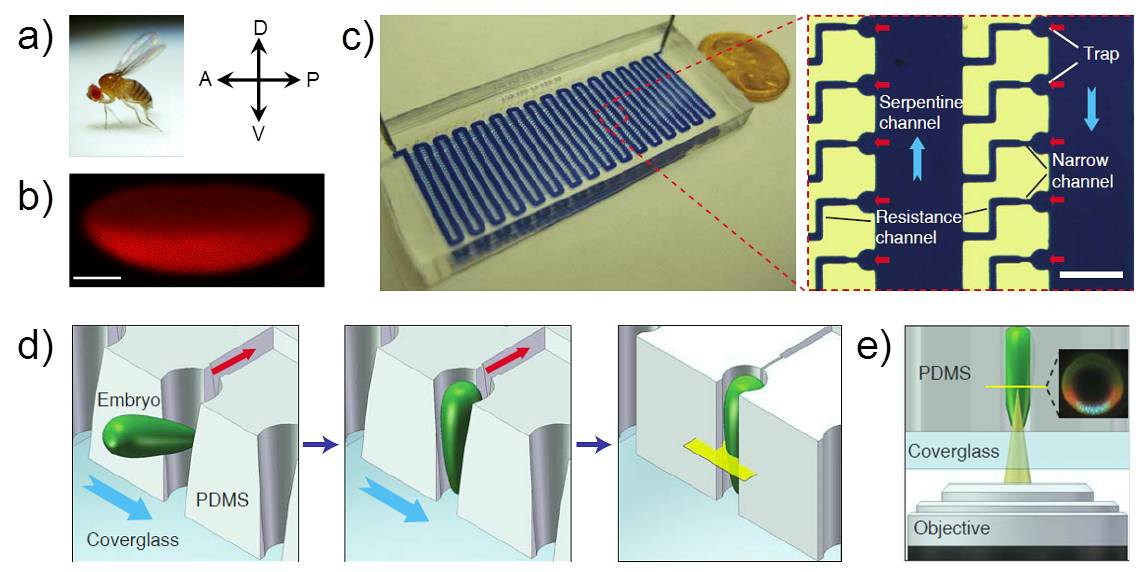
\includegraphics[width=0.65\textwidth]{drosophila_imaging_setup}
\caption{}
\label{subfig:imaging_device}
\end{subfigure}
\begin{subfigure}{0.55\textwidth}
\includegraphics[width=0.8\textwidth]{drosophila_schematic}\\
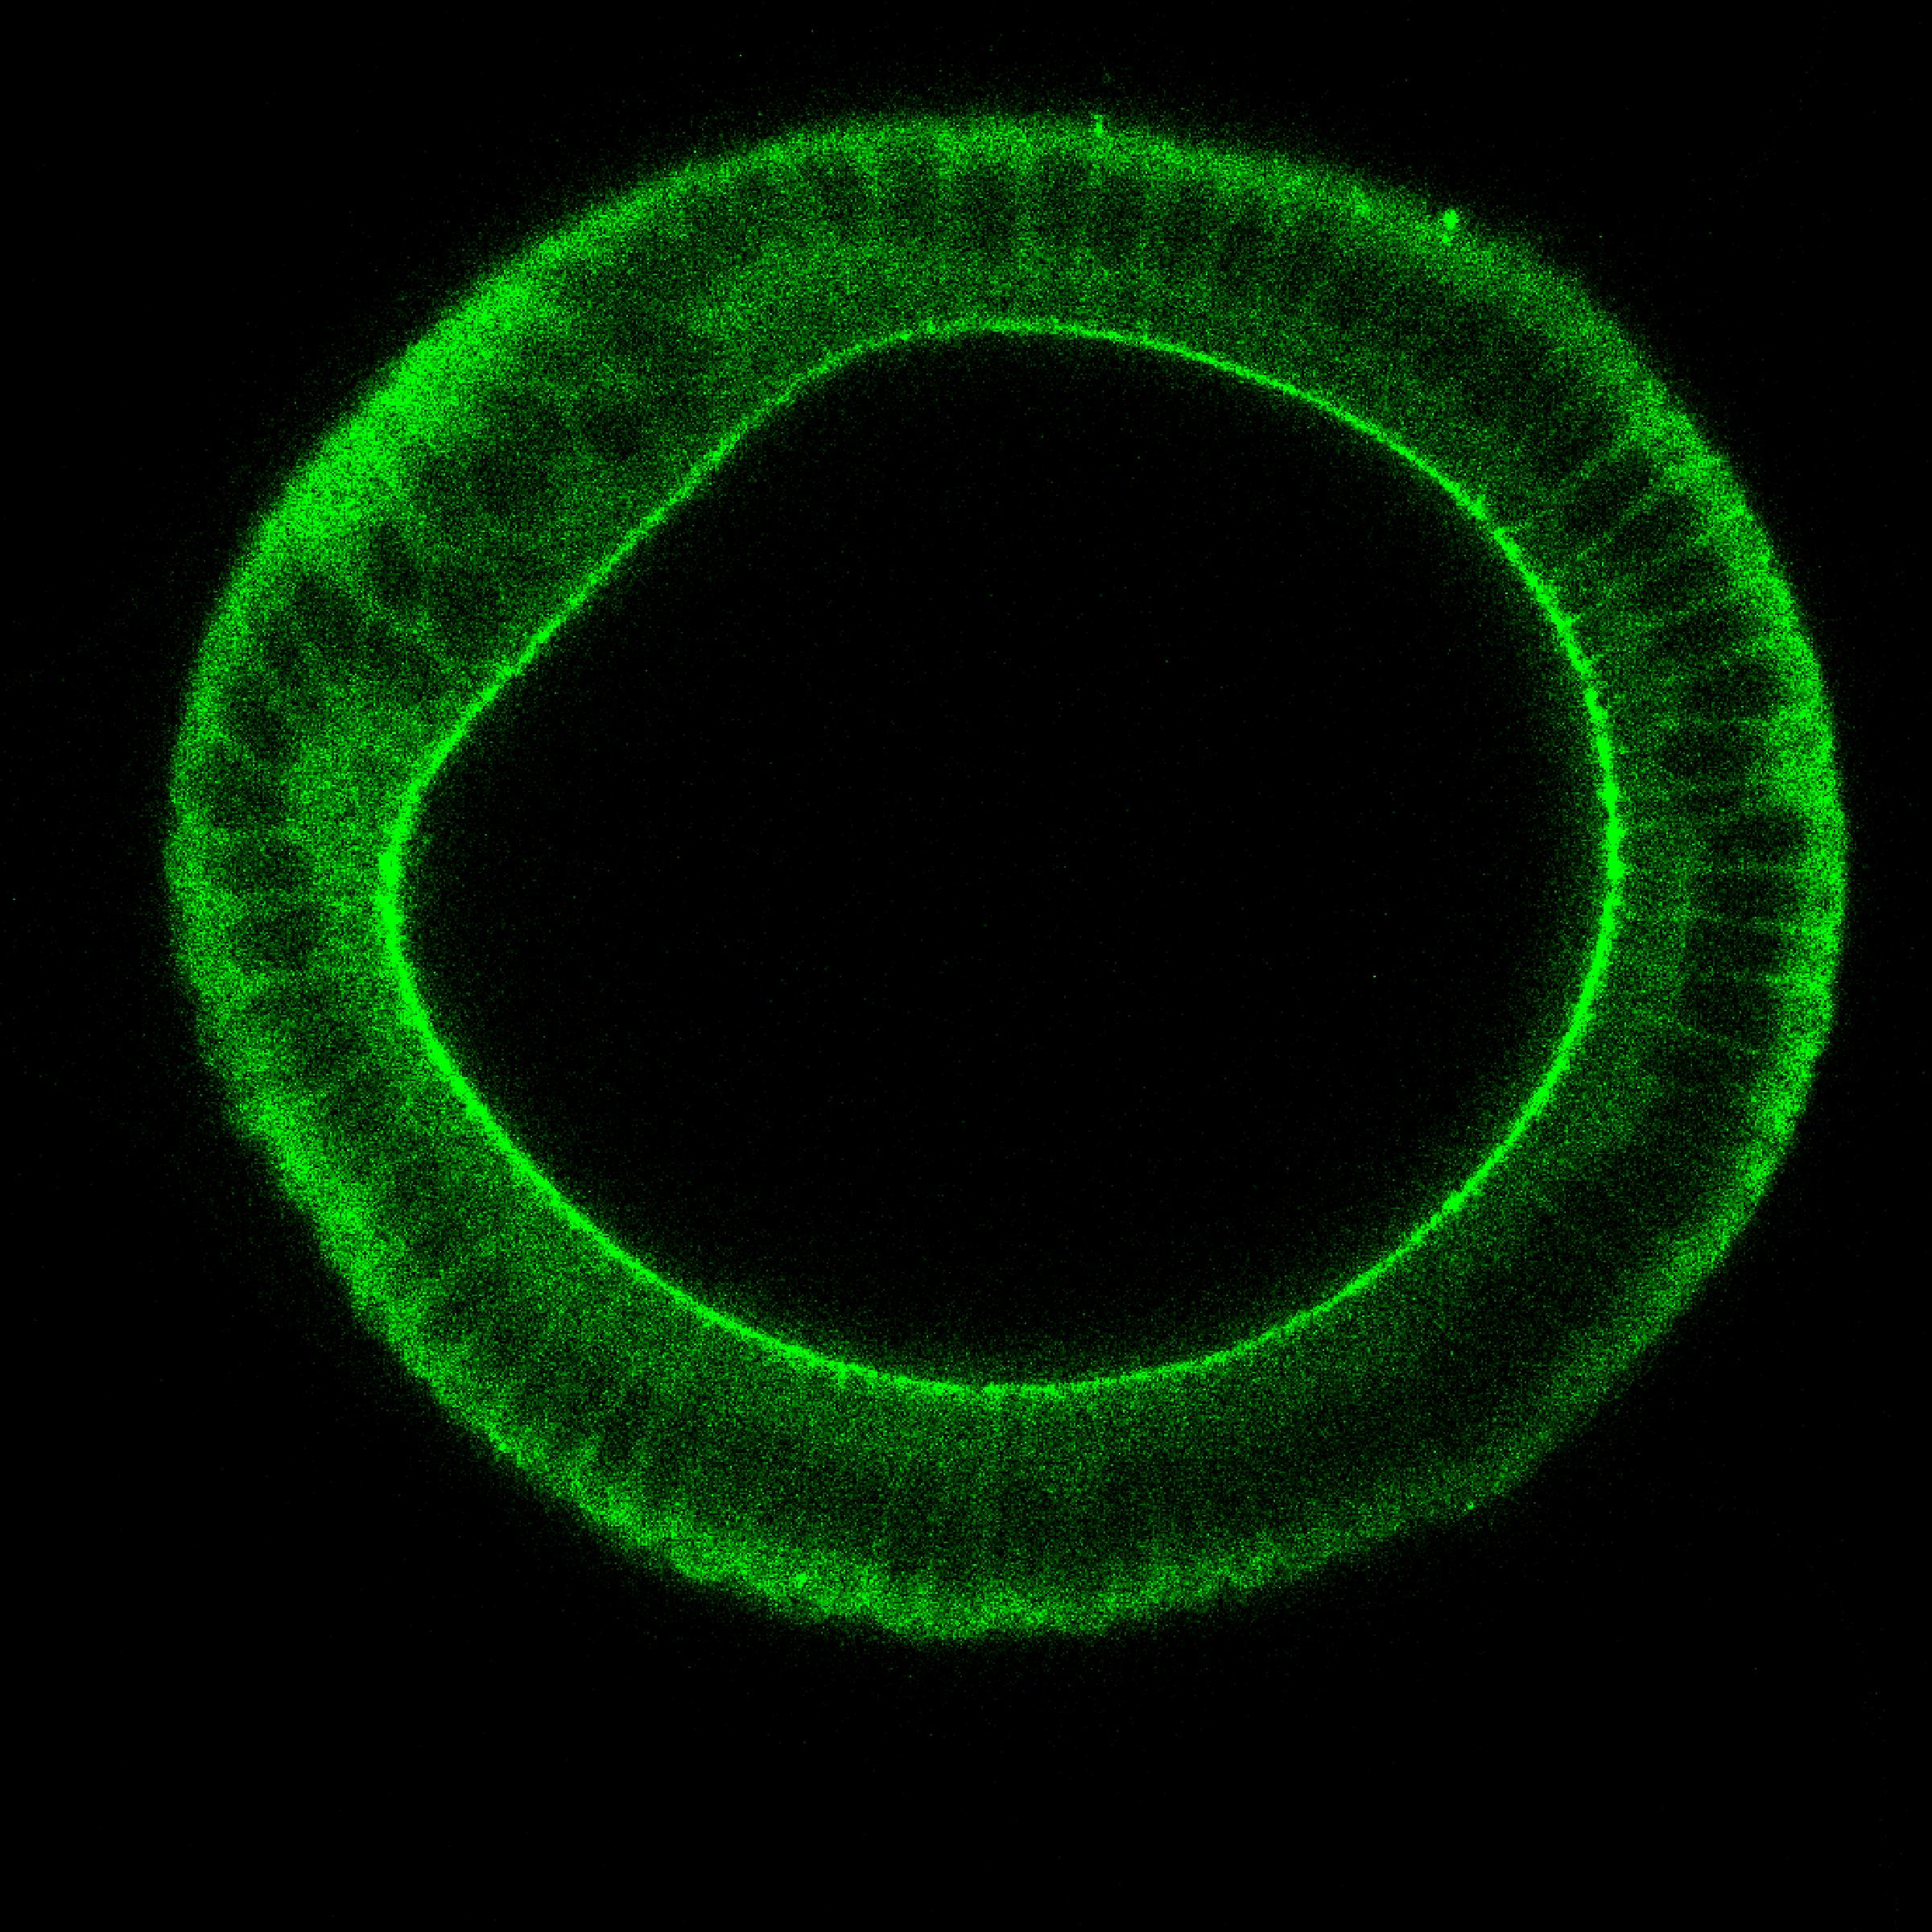
\includegraphics[width=0.25\textwidth]{drosophila_membrane}
\hfill
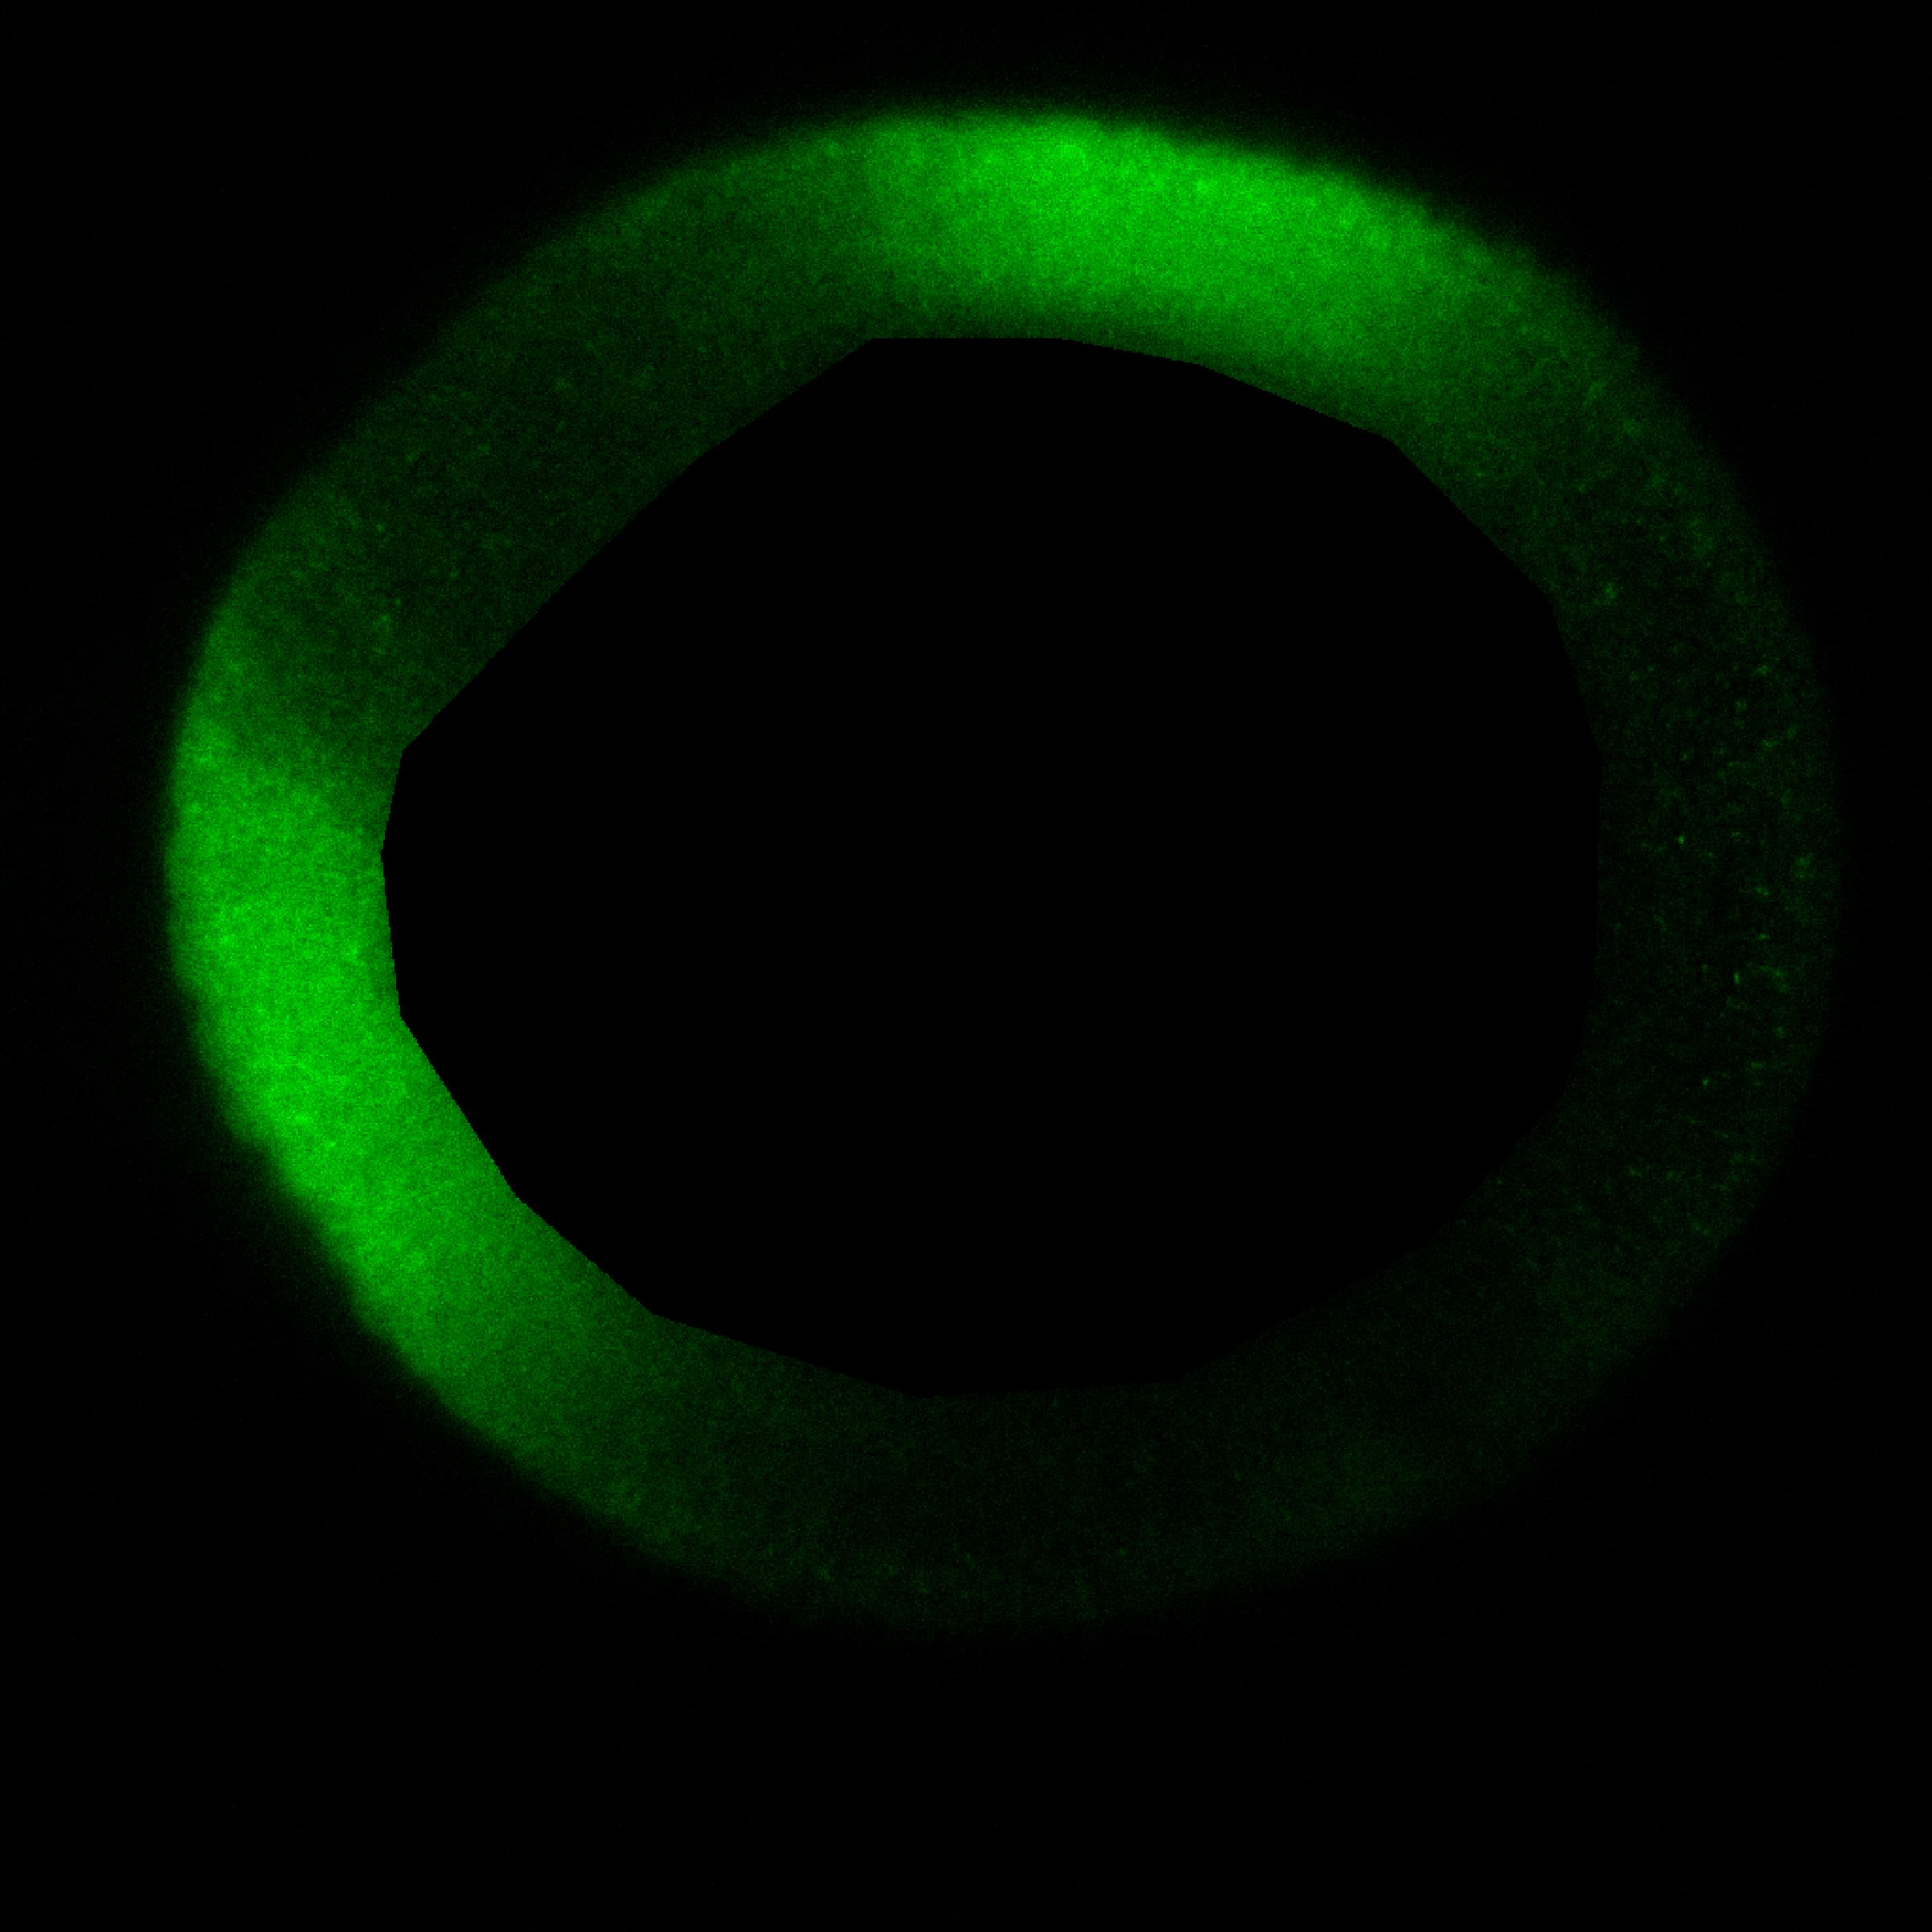
\includegraphics[width=0.25\textwidth]{drosophila_dpERK}
\hfill
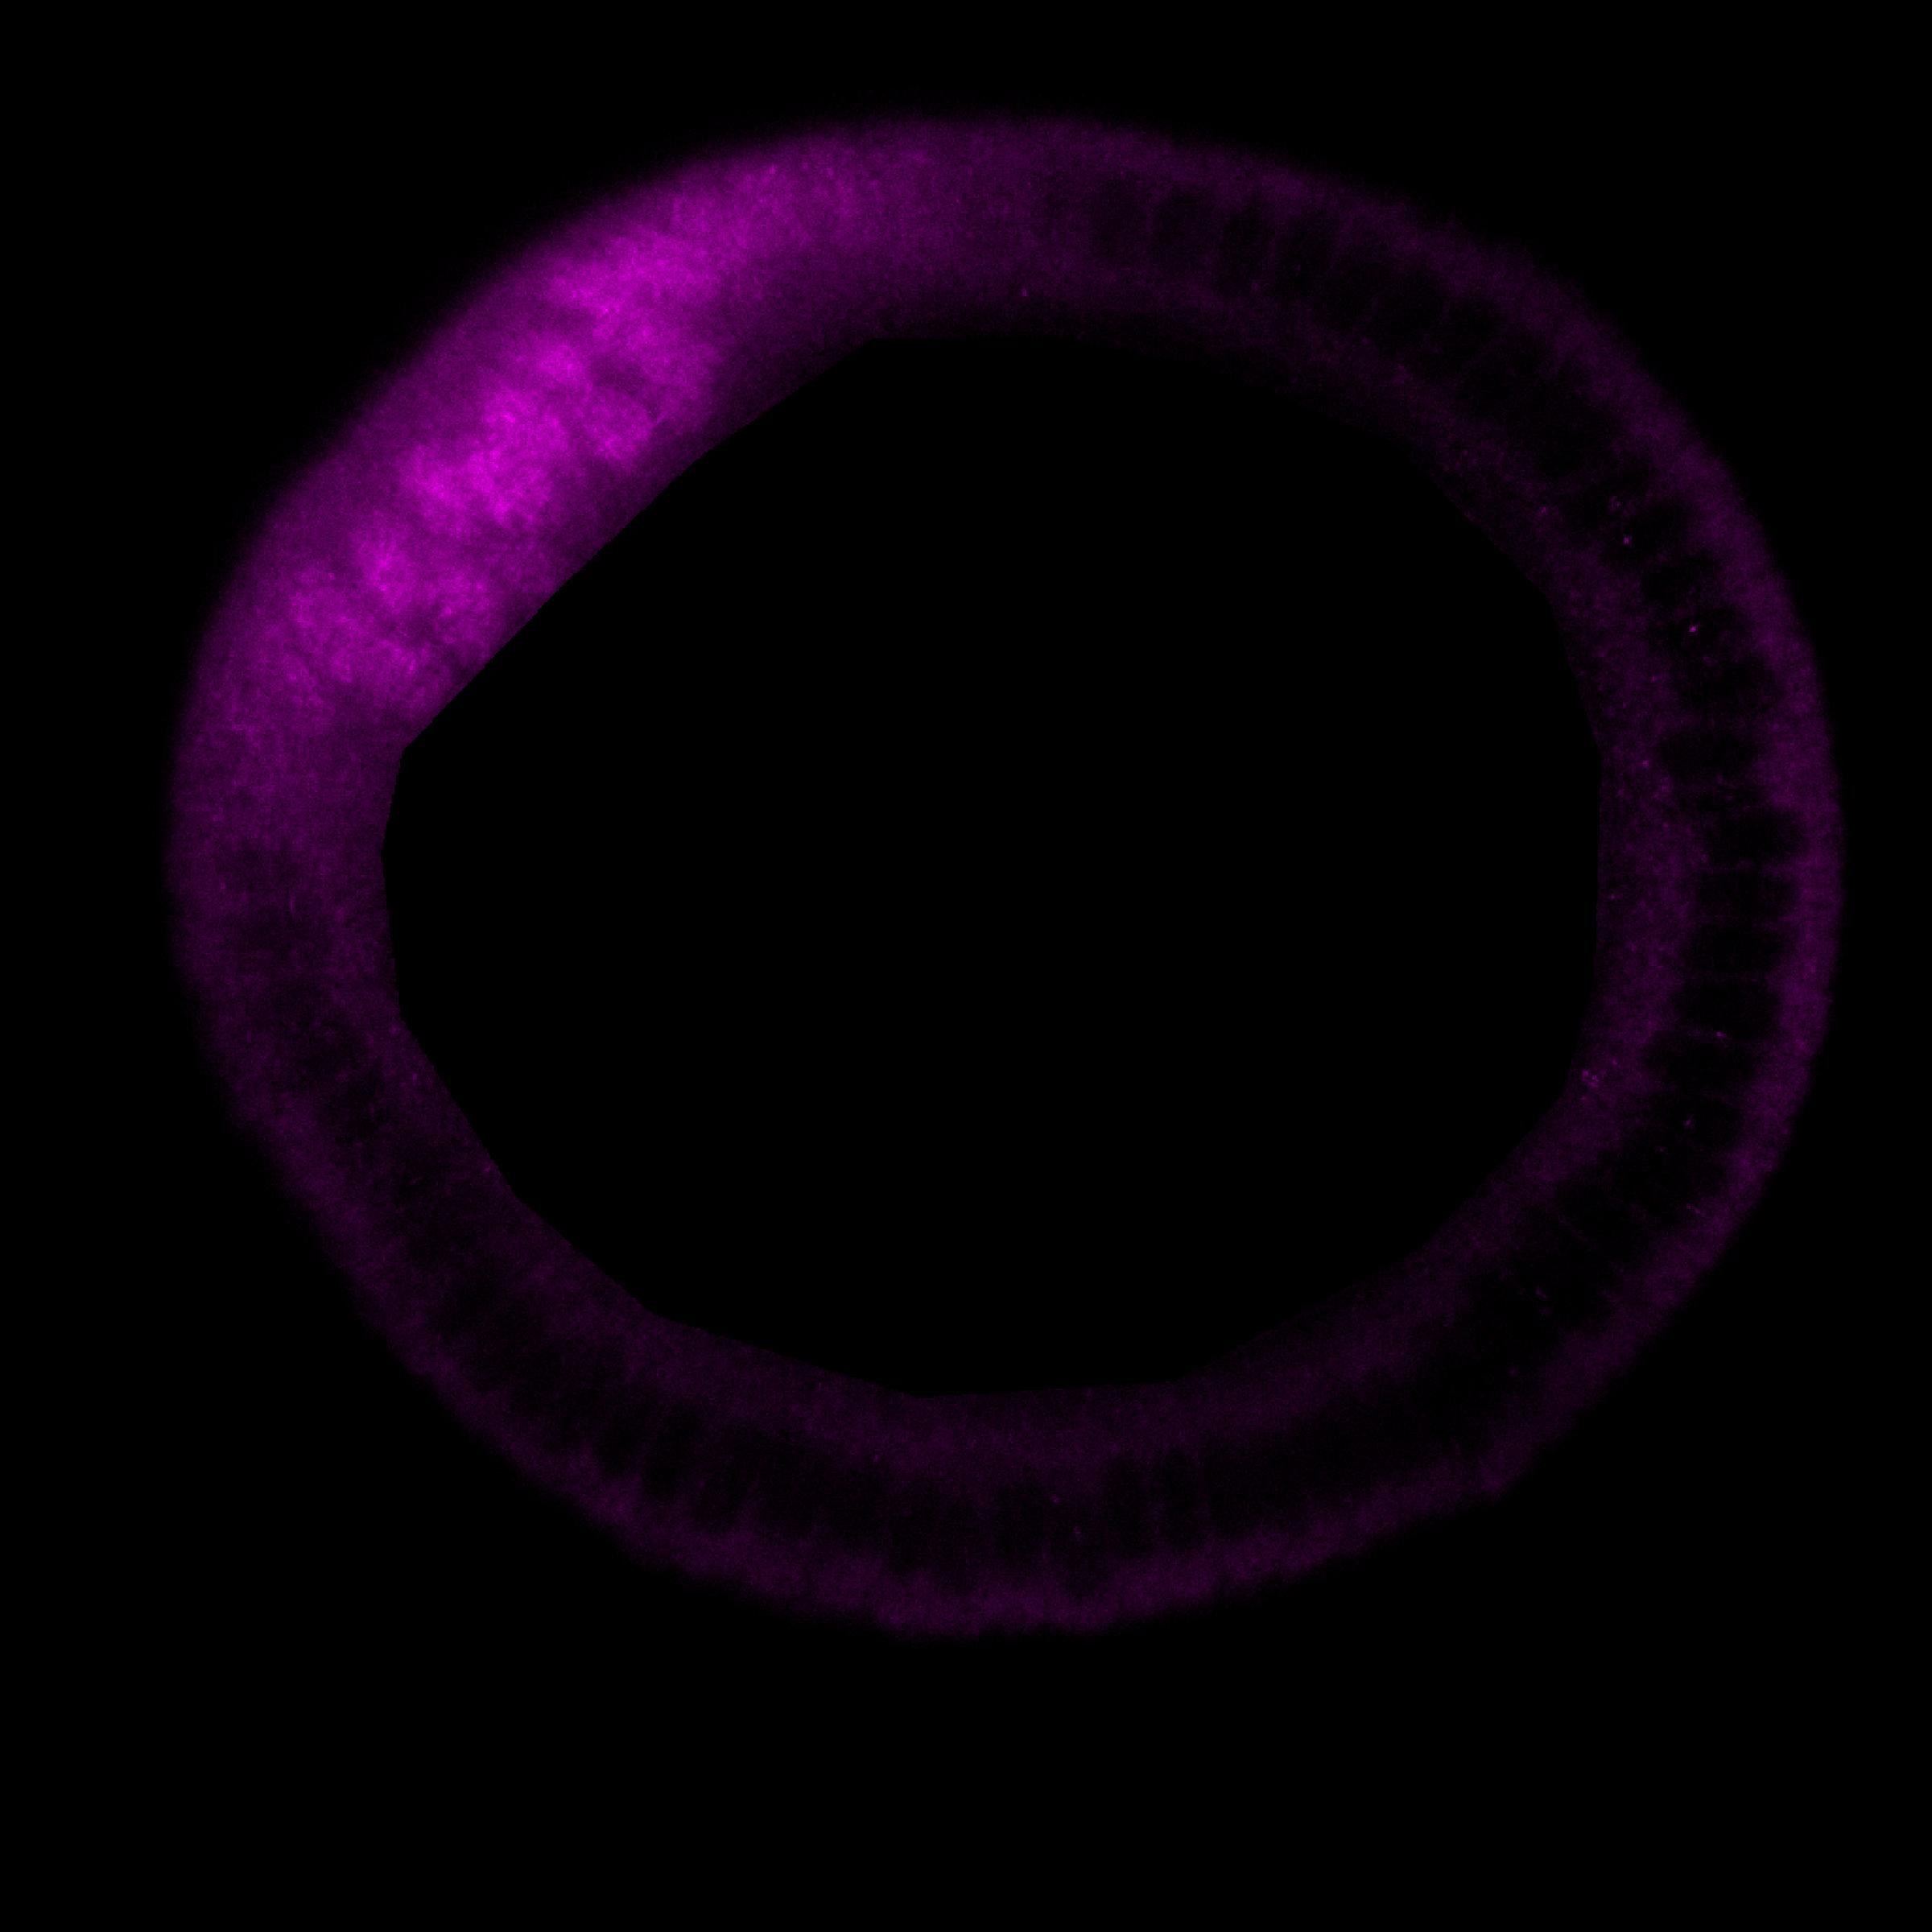
\includegraphics[width=0.25\textwidth]{drosophila_DI}
\caption{}
\end{subfigure}
\begin{subfigure}{0.35\textwidth}
\centering
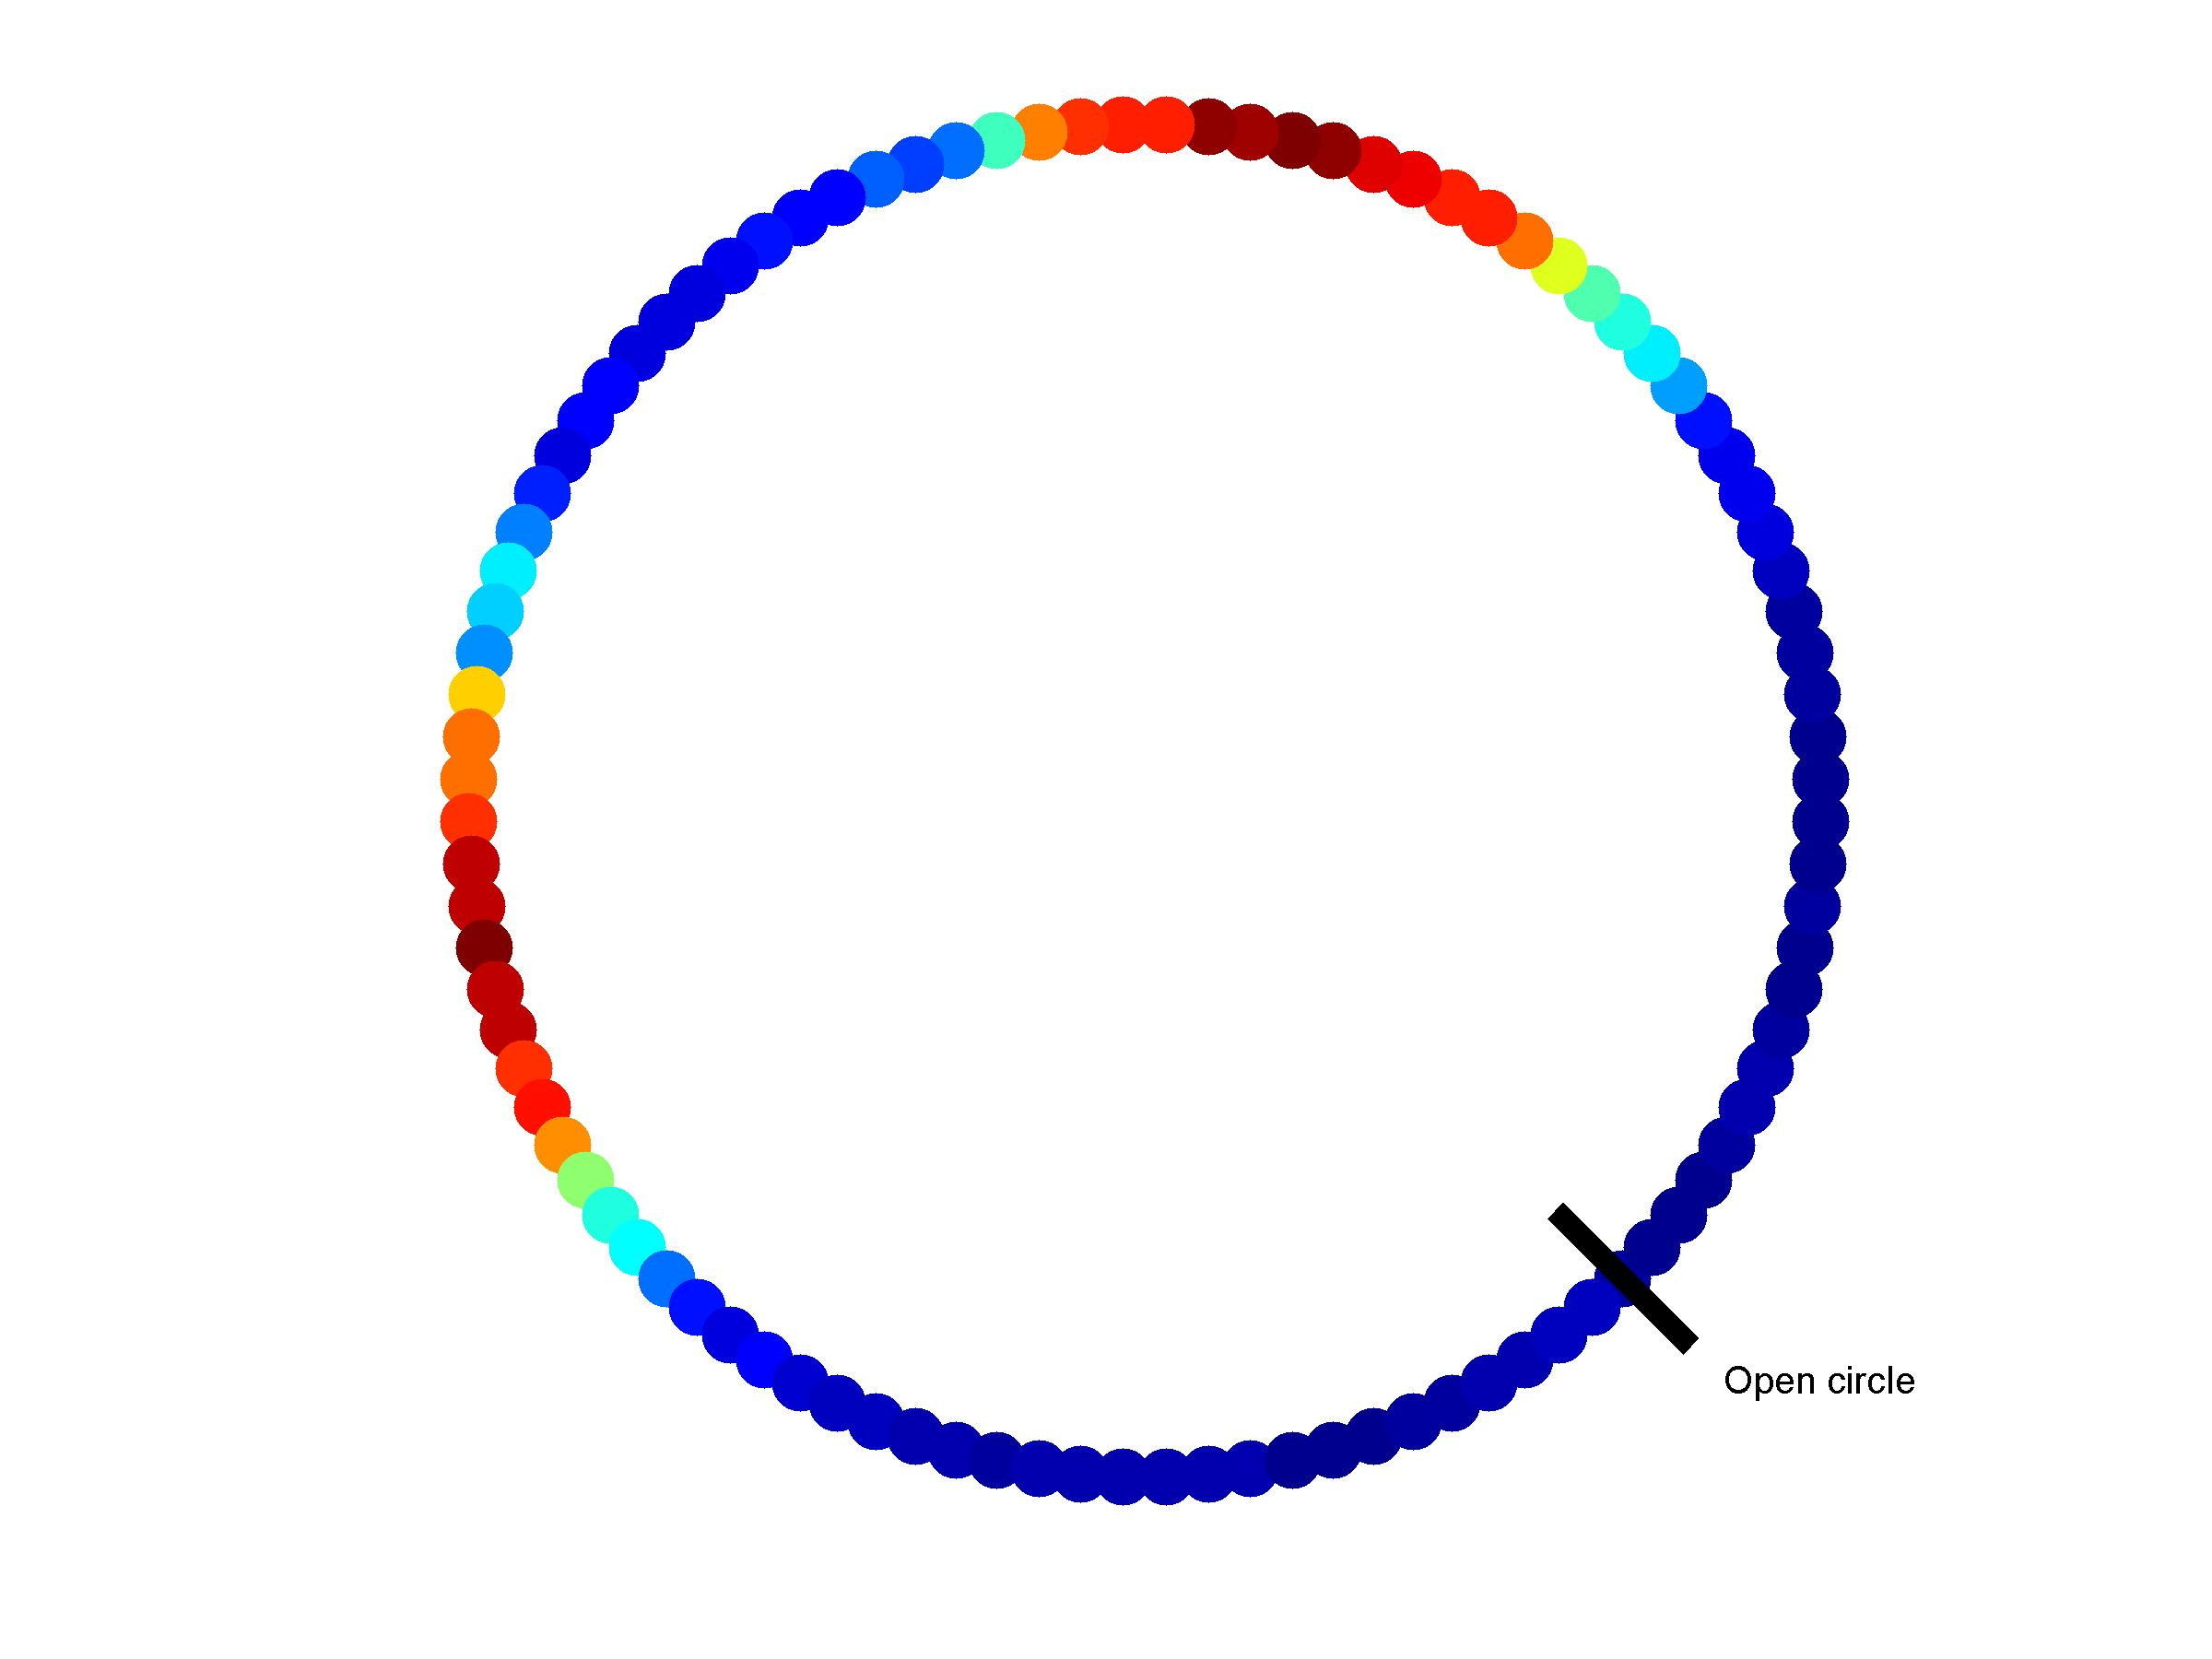
\includegraphics[width=0.7\textwidth]{circle_profile}\\
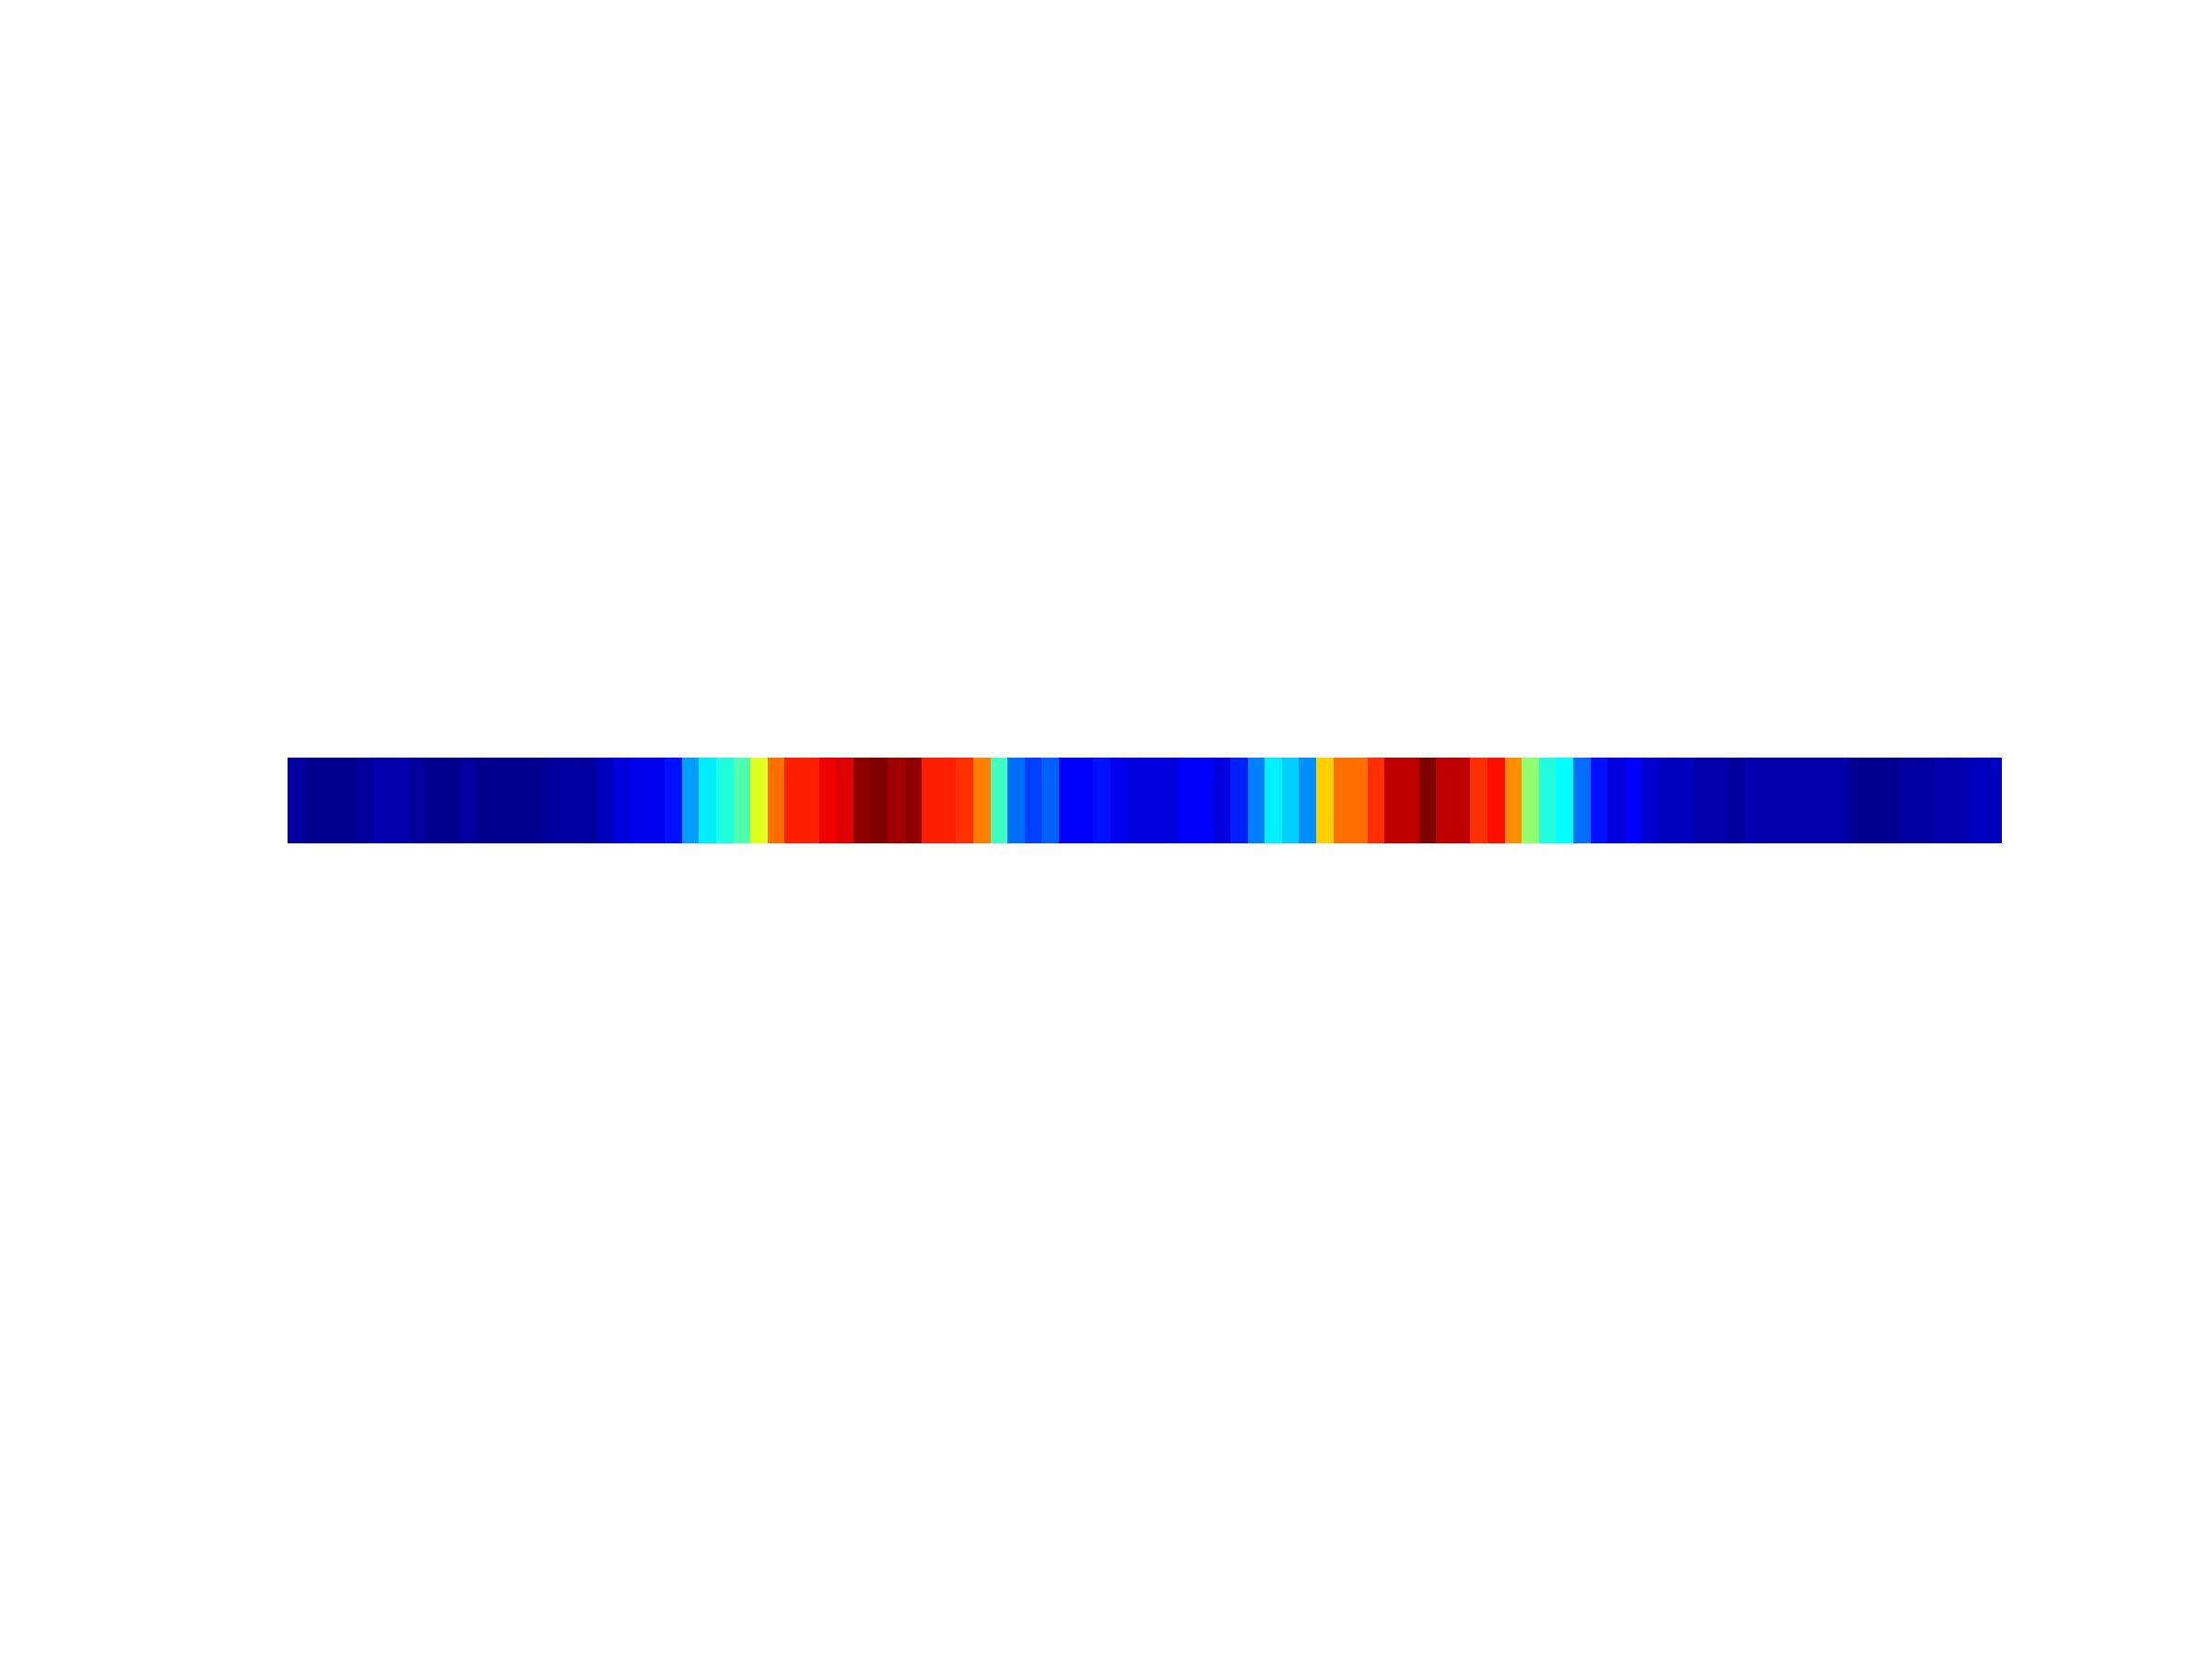
\includegraphics[width=\textwidth, trim=0mm 300mm 0mm 200mm, clip]{line_profile}
\caption{}
\end{subfigure}\\
\begin{subfigure}{0.4\textwidth}
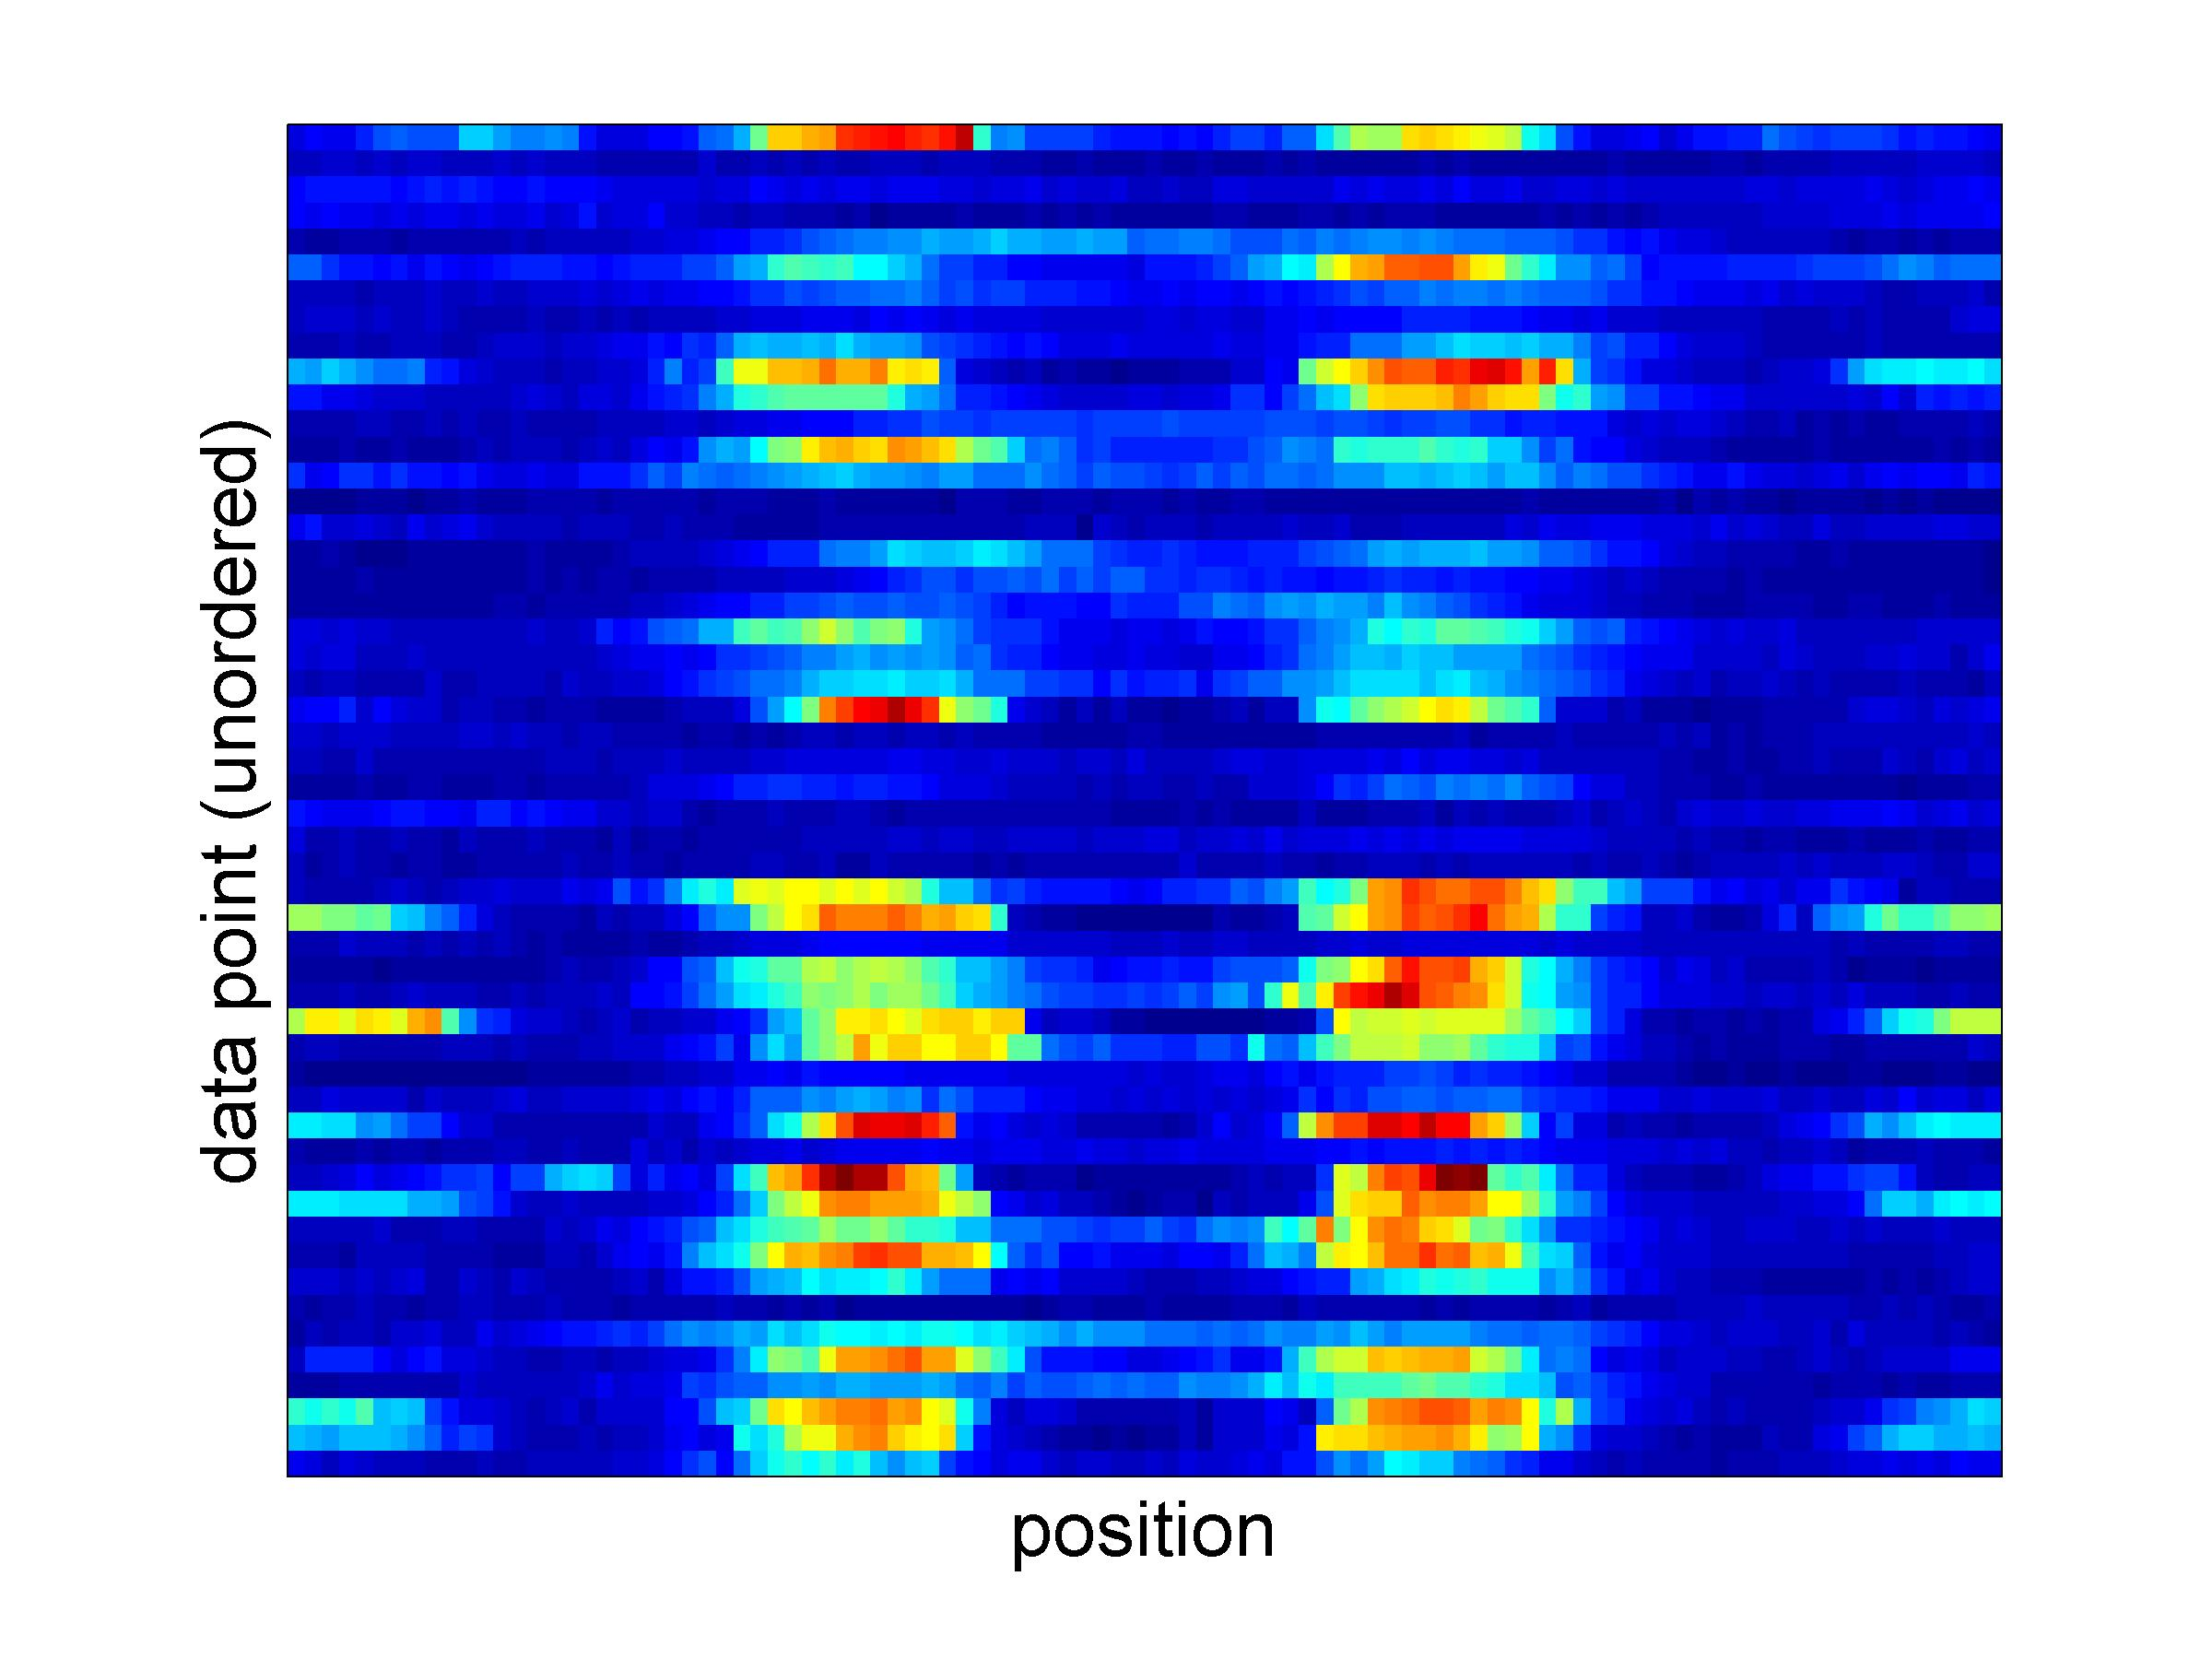
\includegraphics[width=\textwidth]{data_unordered}
\caption{}
\end{subfigure}
\begin{subfigure}{0.4\textwidth}
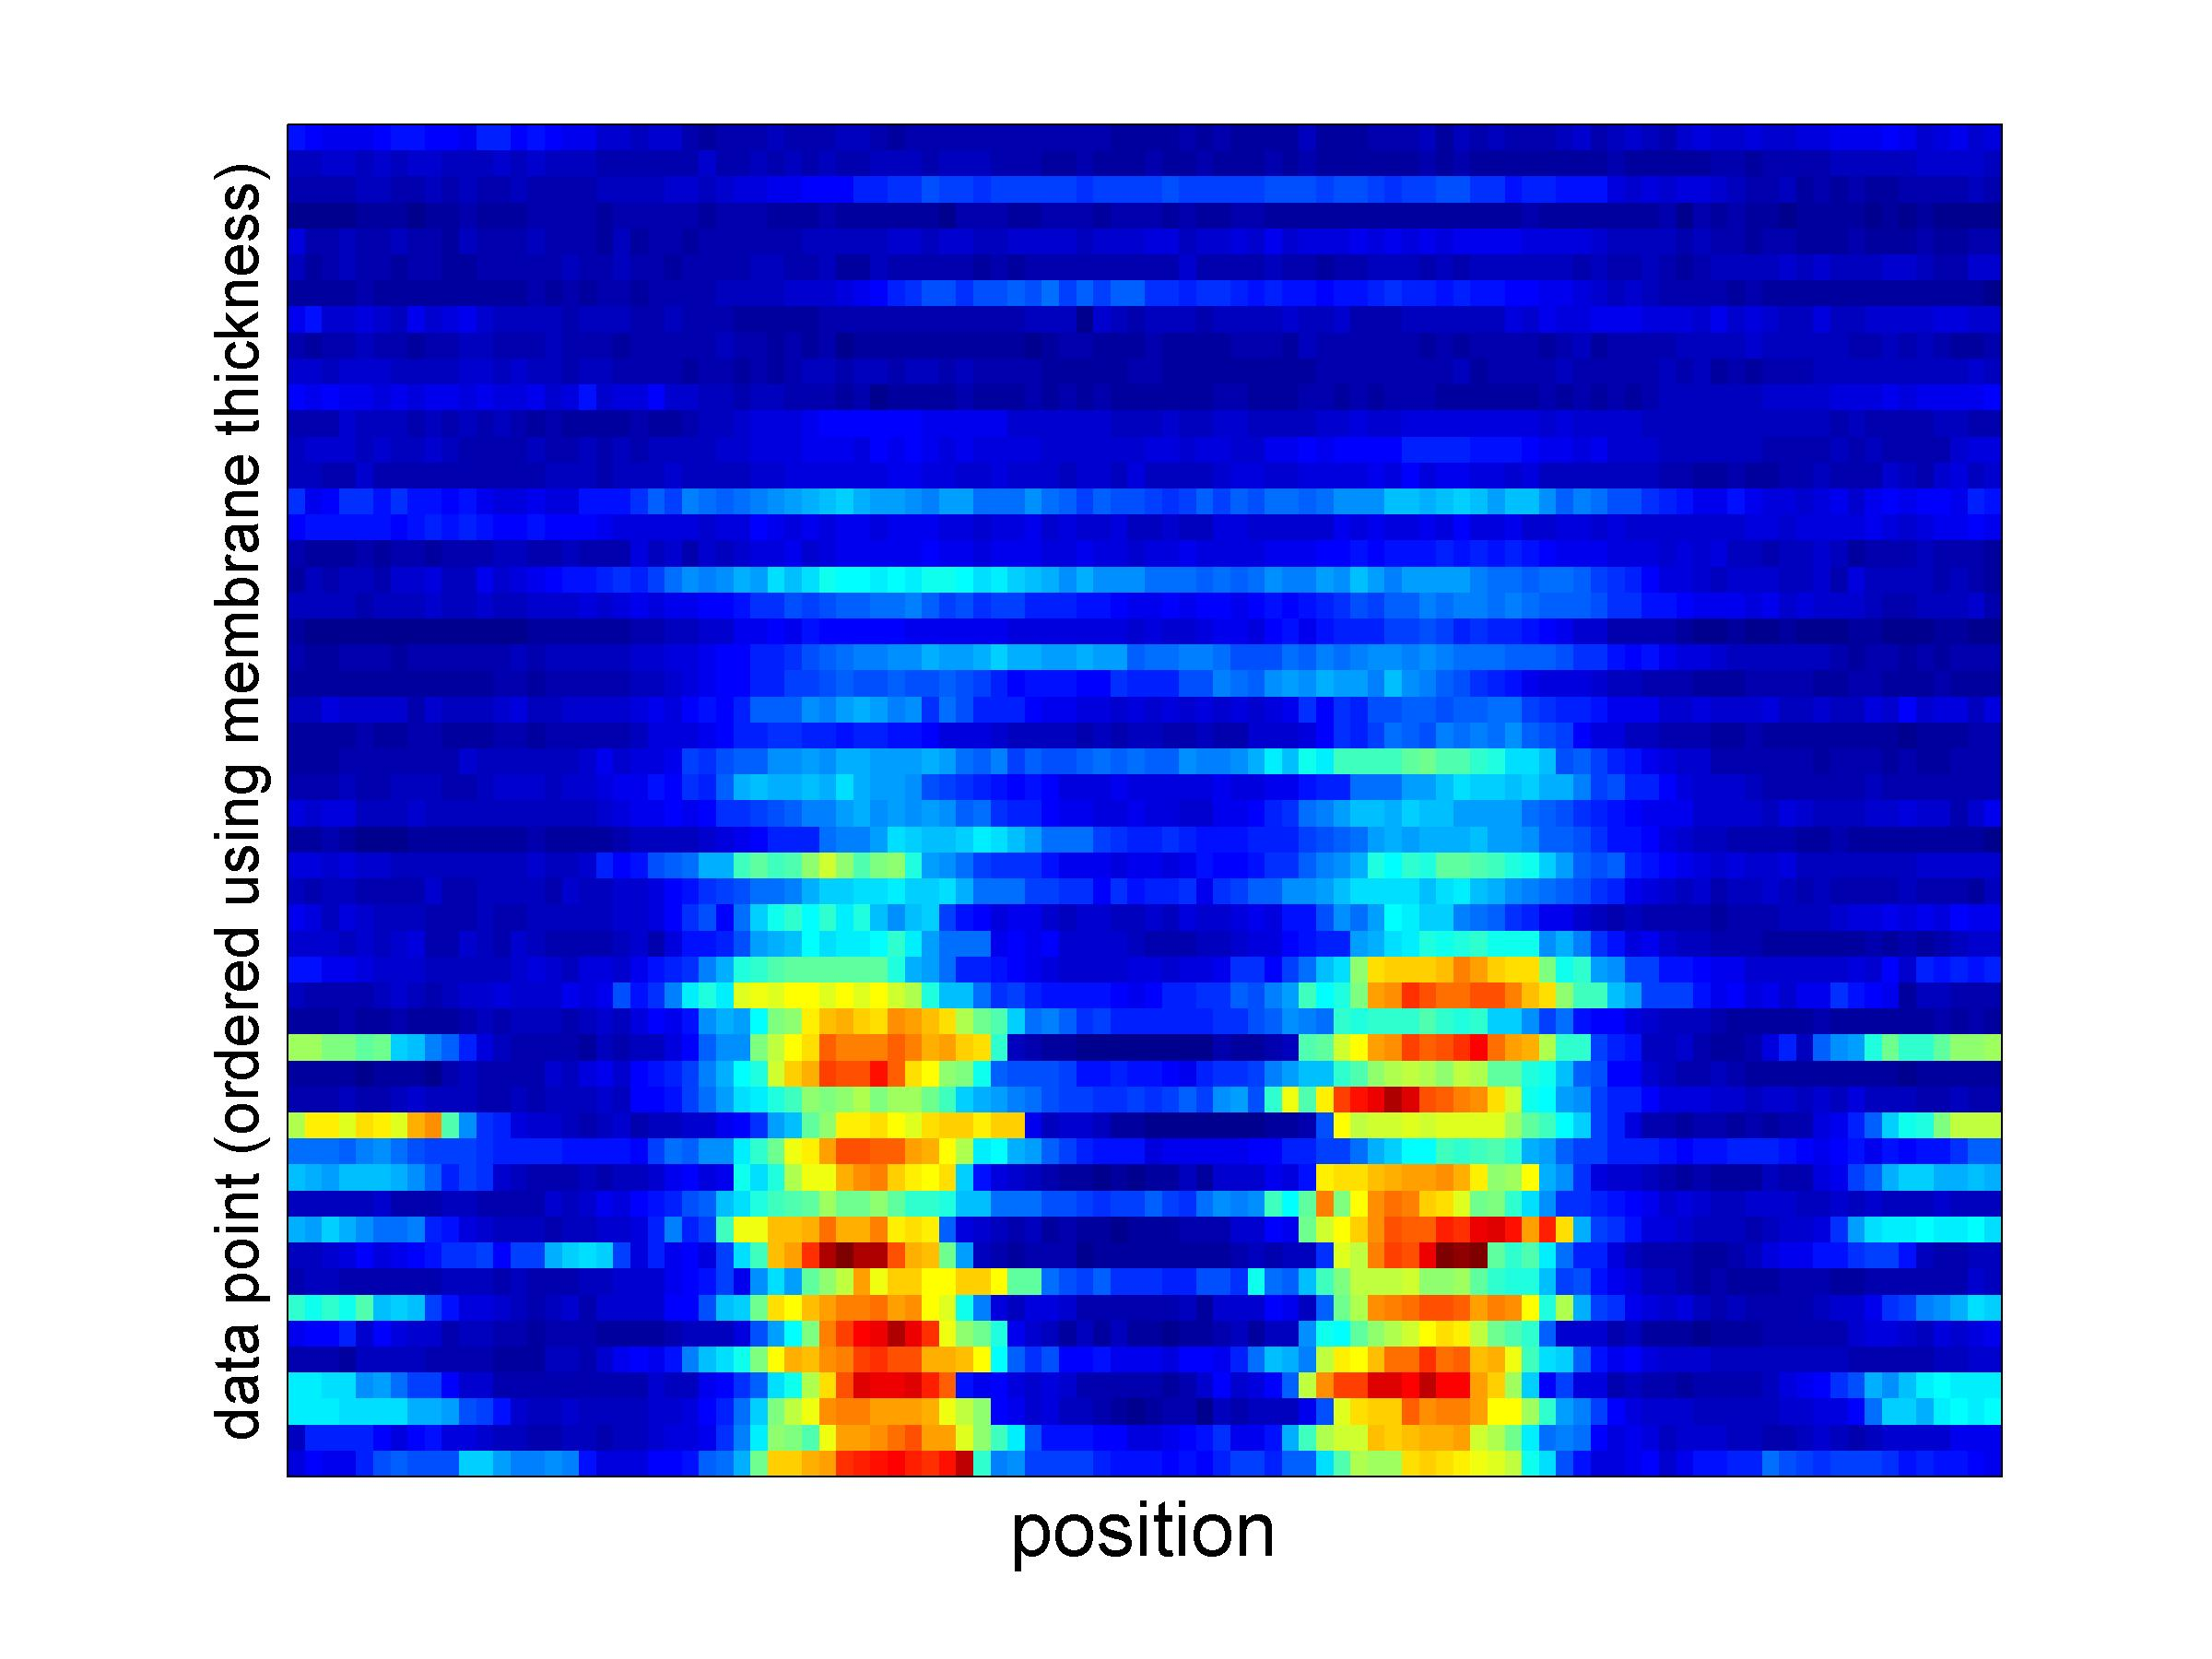
\includegraphics[width=\textwidth]{data_ordered_membrane}
\caption{}
\end{subfigure}
\end{center}
\caption{{\bf Data collection.} (a) Schematic of {\em Drosophila} embryo (longitudinal and cross-section), and cross-sectional fluorescent images of an embryo stained for the membrane proteins (left), dpERK (center), and dorsal protein (right).
(b) Concentration profile of dpERK extracted from a fluorescent image. The circular profile is ``unwrapped'' at the dorsal midline (determined from the expression of the dorsal protein) to obtain a concentration profile on a line.
(c) Concentration profiles of dpERK for many embryos. Each row represents a different embryo fixed at a slightly different developmental time.
(d) Concentration profiles of dpERK for many embryos from (c), now ordered by the thickness of the membrane. The membrane thickness is known to be one-to-one with time.}
\label{fig:background}
\end{figure}

Here,  we will discuss alternative methodologies to reconstruct the dpERK dynamics from fluorescent images. 
%
%TODO: add why we cannot always do the procedure outlined above
We will use various dimensionality techniques to {\em automatically} order the dpERK concentration profiles in time.
%
We assume that the data is approximately one-dimensional, and that this one dimension parameterizes time, so that reducing the data to one dimension and ordering it along this dimension will (approximately) order it in time. 
%
We will not only focus on the linear concentration profiles extracted from the images, but also work directly with the two-dimensional dpERK fluorescent images. 
%
Finally, we will look at ordering the two-dimensional membrane images in time; these are much more feature-rich than the dpERK images, and prove to be more challenging.

% Results and Discussion can be combined.
\section*{Results}

\subsection*{dpERK concentration profiles ordered using principal component analysis}

We first used principal components analysis (PCA) to order the one-dimensional concentration profiles in time. 
%
We computed the first principal component, $\psi_1$, from the data set of concentration profiles, and ordered the data by the projection coefficients onto $\psi_1$.
%
The results are shown in Figure \ref{fig:PCA_ordering}.
%
There is a strong correlation between the first projection coefficient, $\langle x_i, \psi_1 \rangle$, and the membrane thickness;
the Spearman correlation between the first projection coefficient and the membrane thickness is 0.9244.

\begin{figure}[!ht]
\begin{subfigure}{0.3\textwidth}
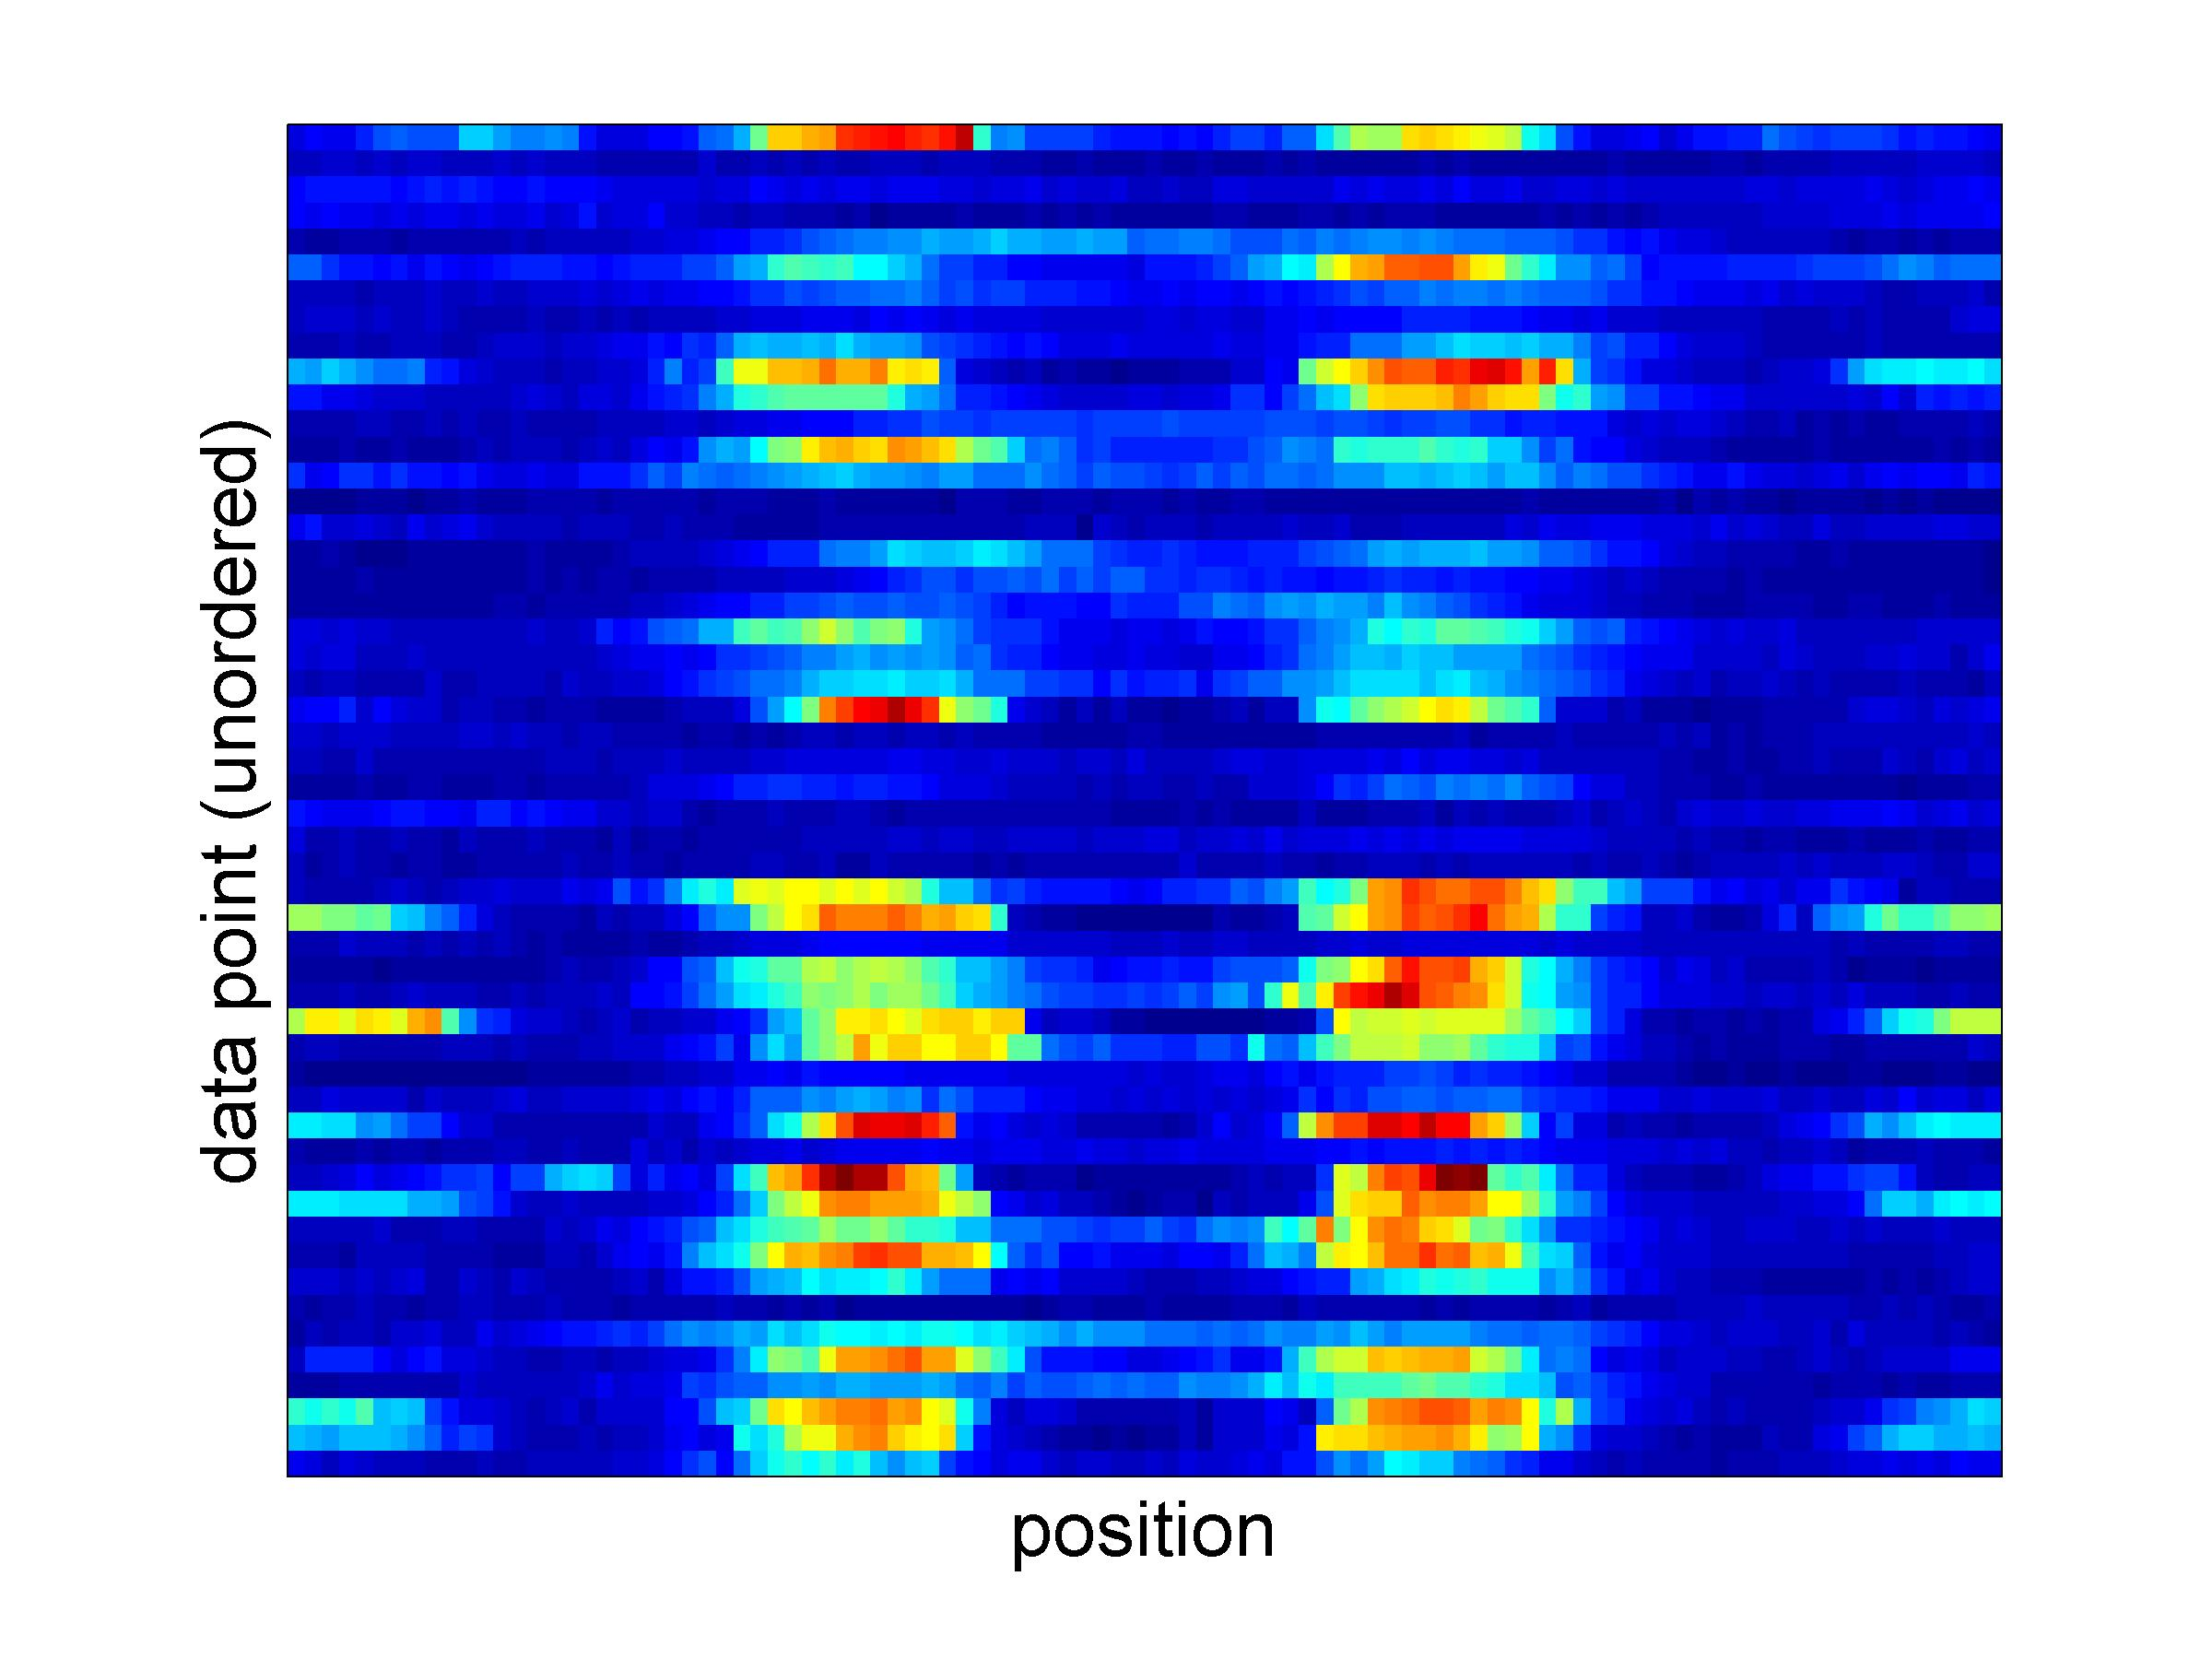
\includegraphics[width=\textwidth]{data_unordered}
\caption{}
\label{subfig:unordered_profiles}
\end{subfigure}
\begin{subfigure}{0.3\textwidth}
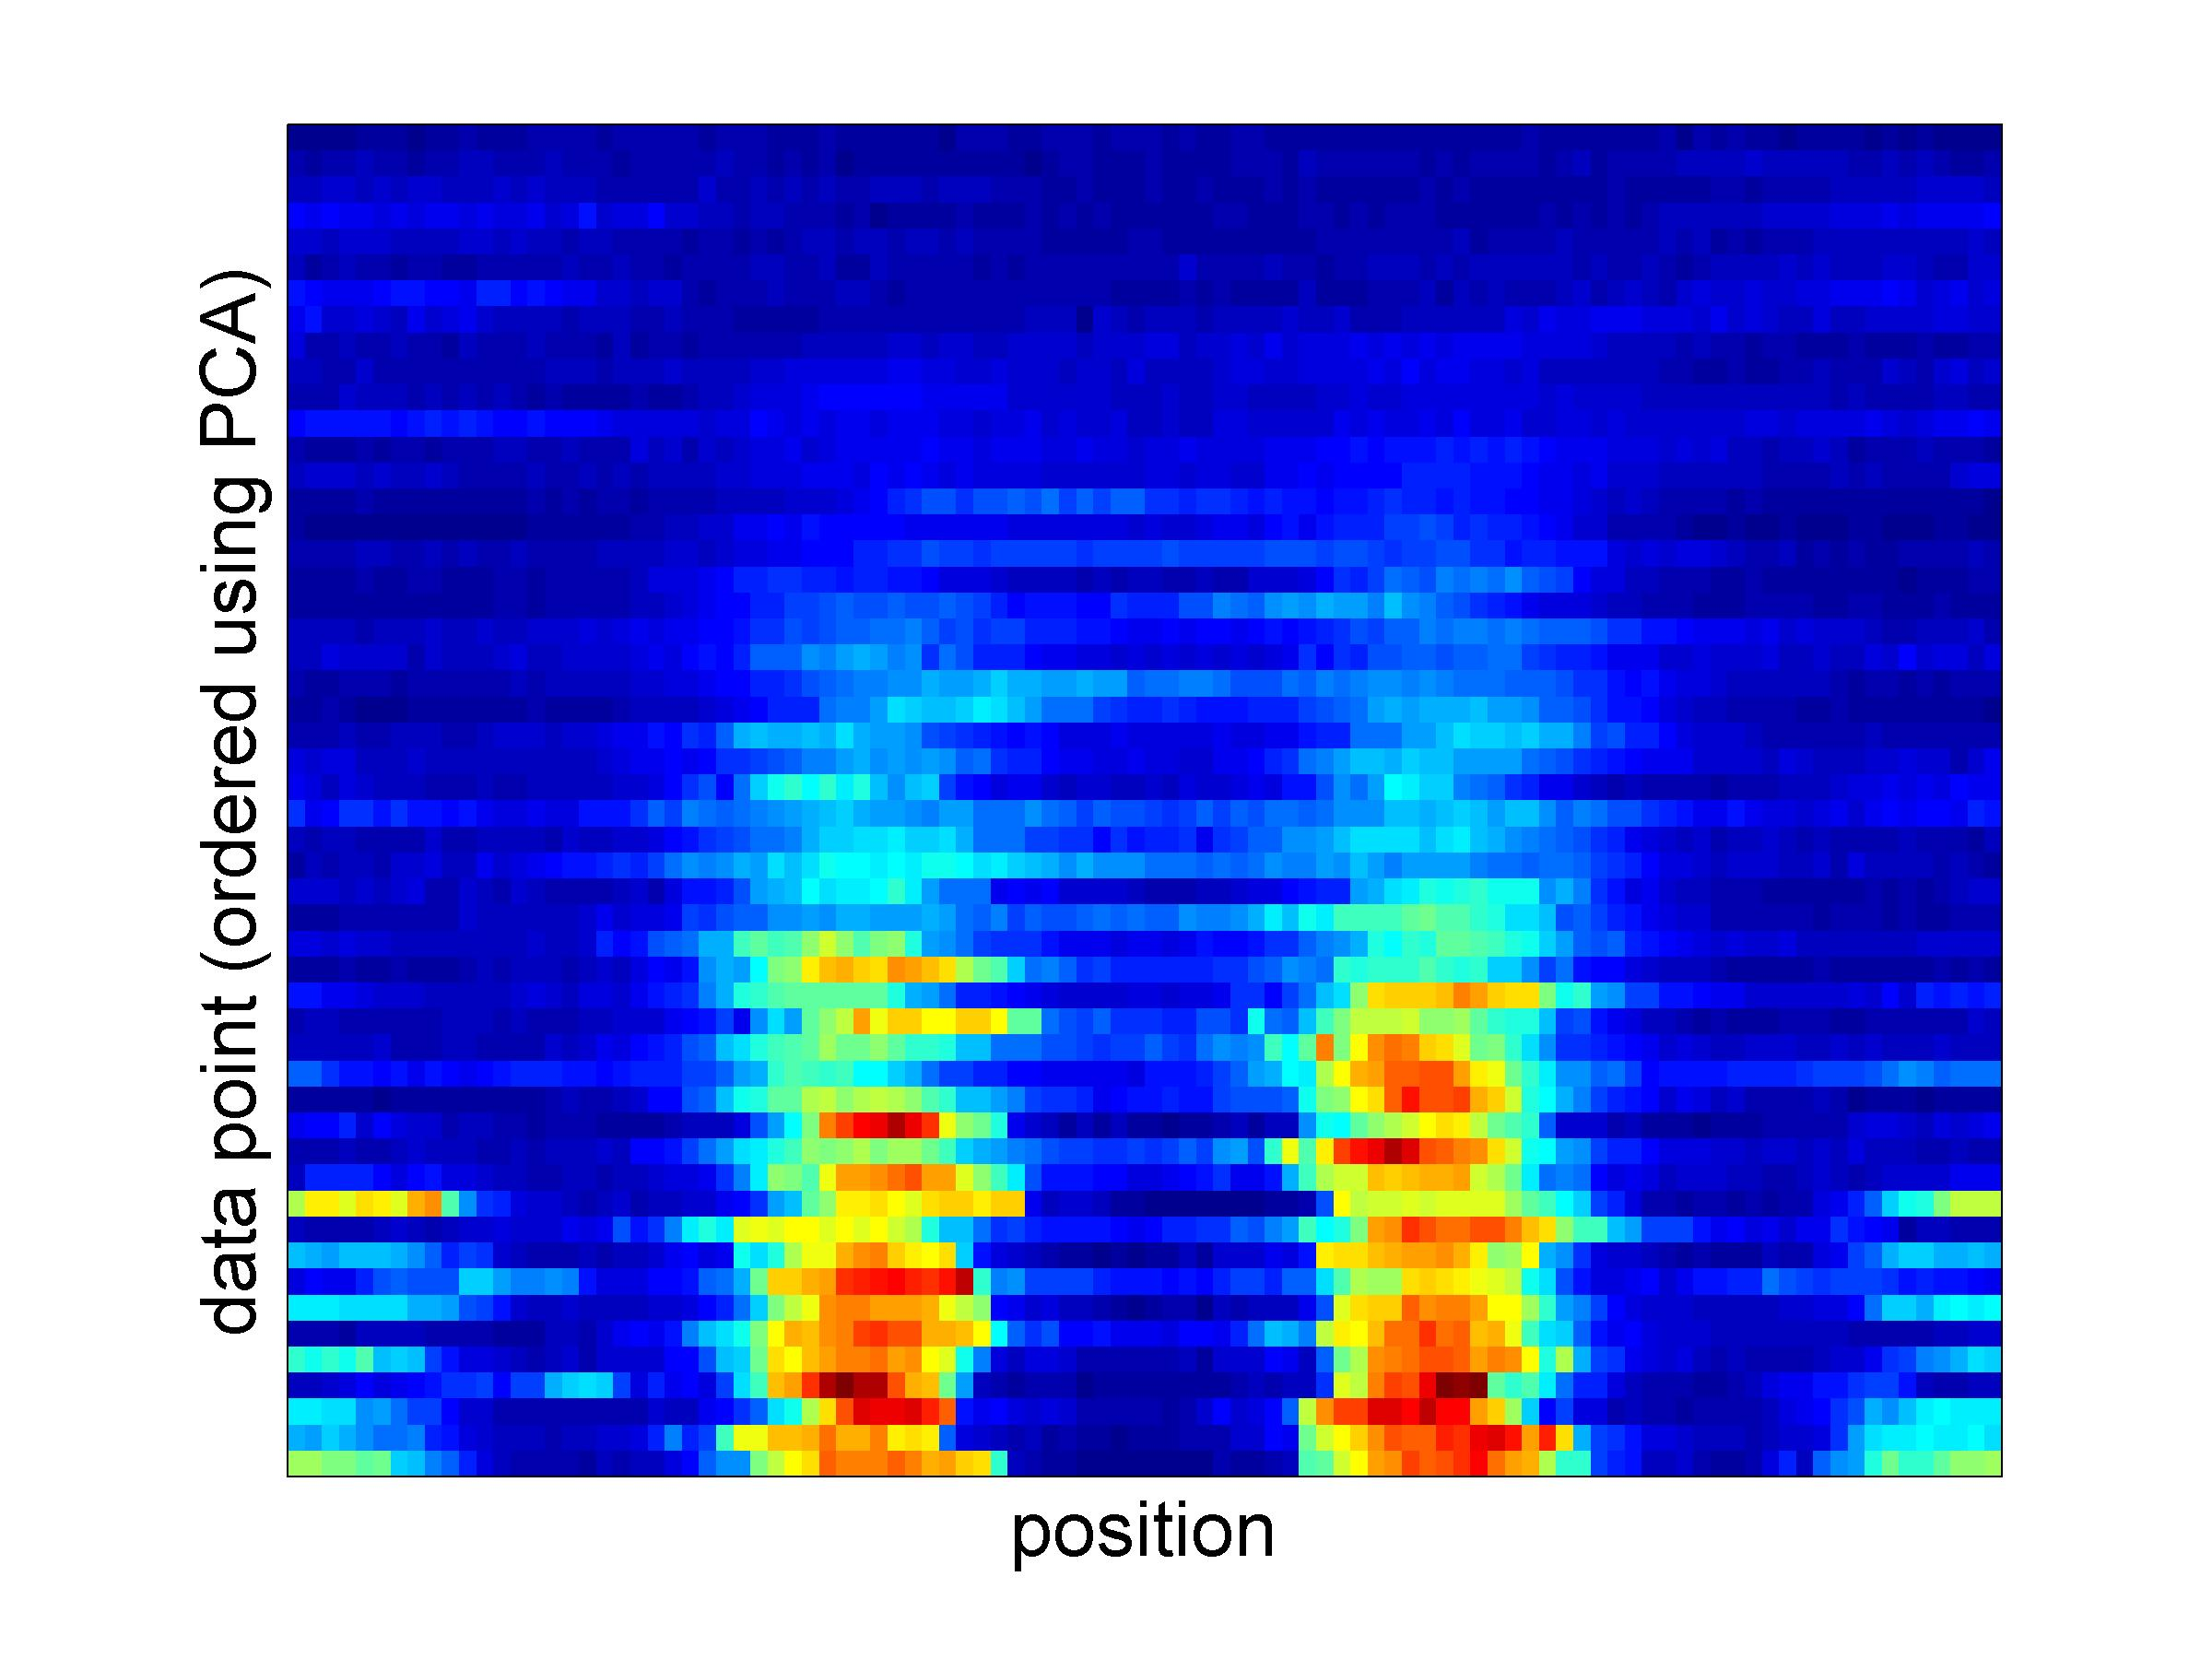
\includegraphics[width=\textwidth]{data_ordered_PCA}
\caption{}
\label{subfig:PCA_ordering_image}
\end{subfigure}
\begin{subfigure}{0.3\textwidth}
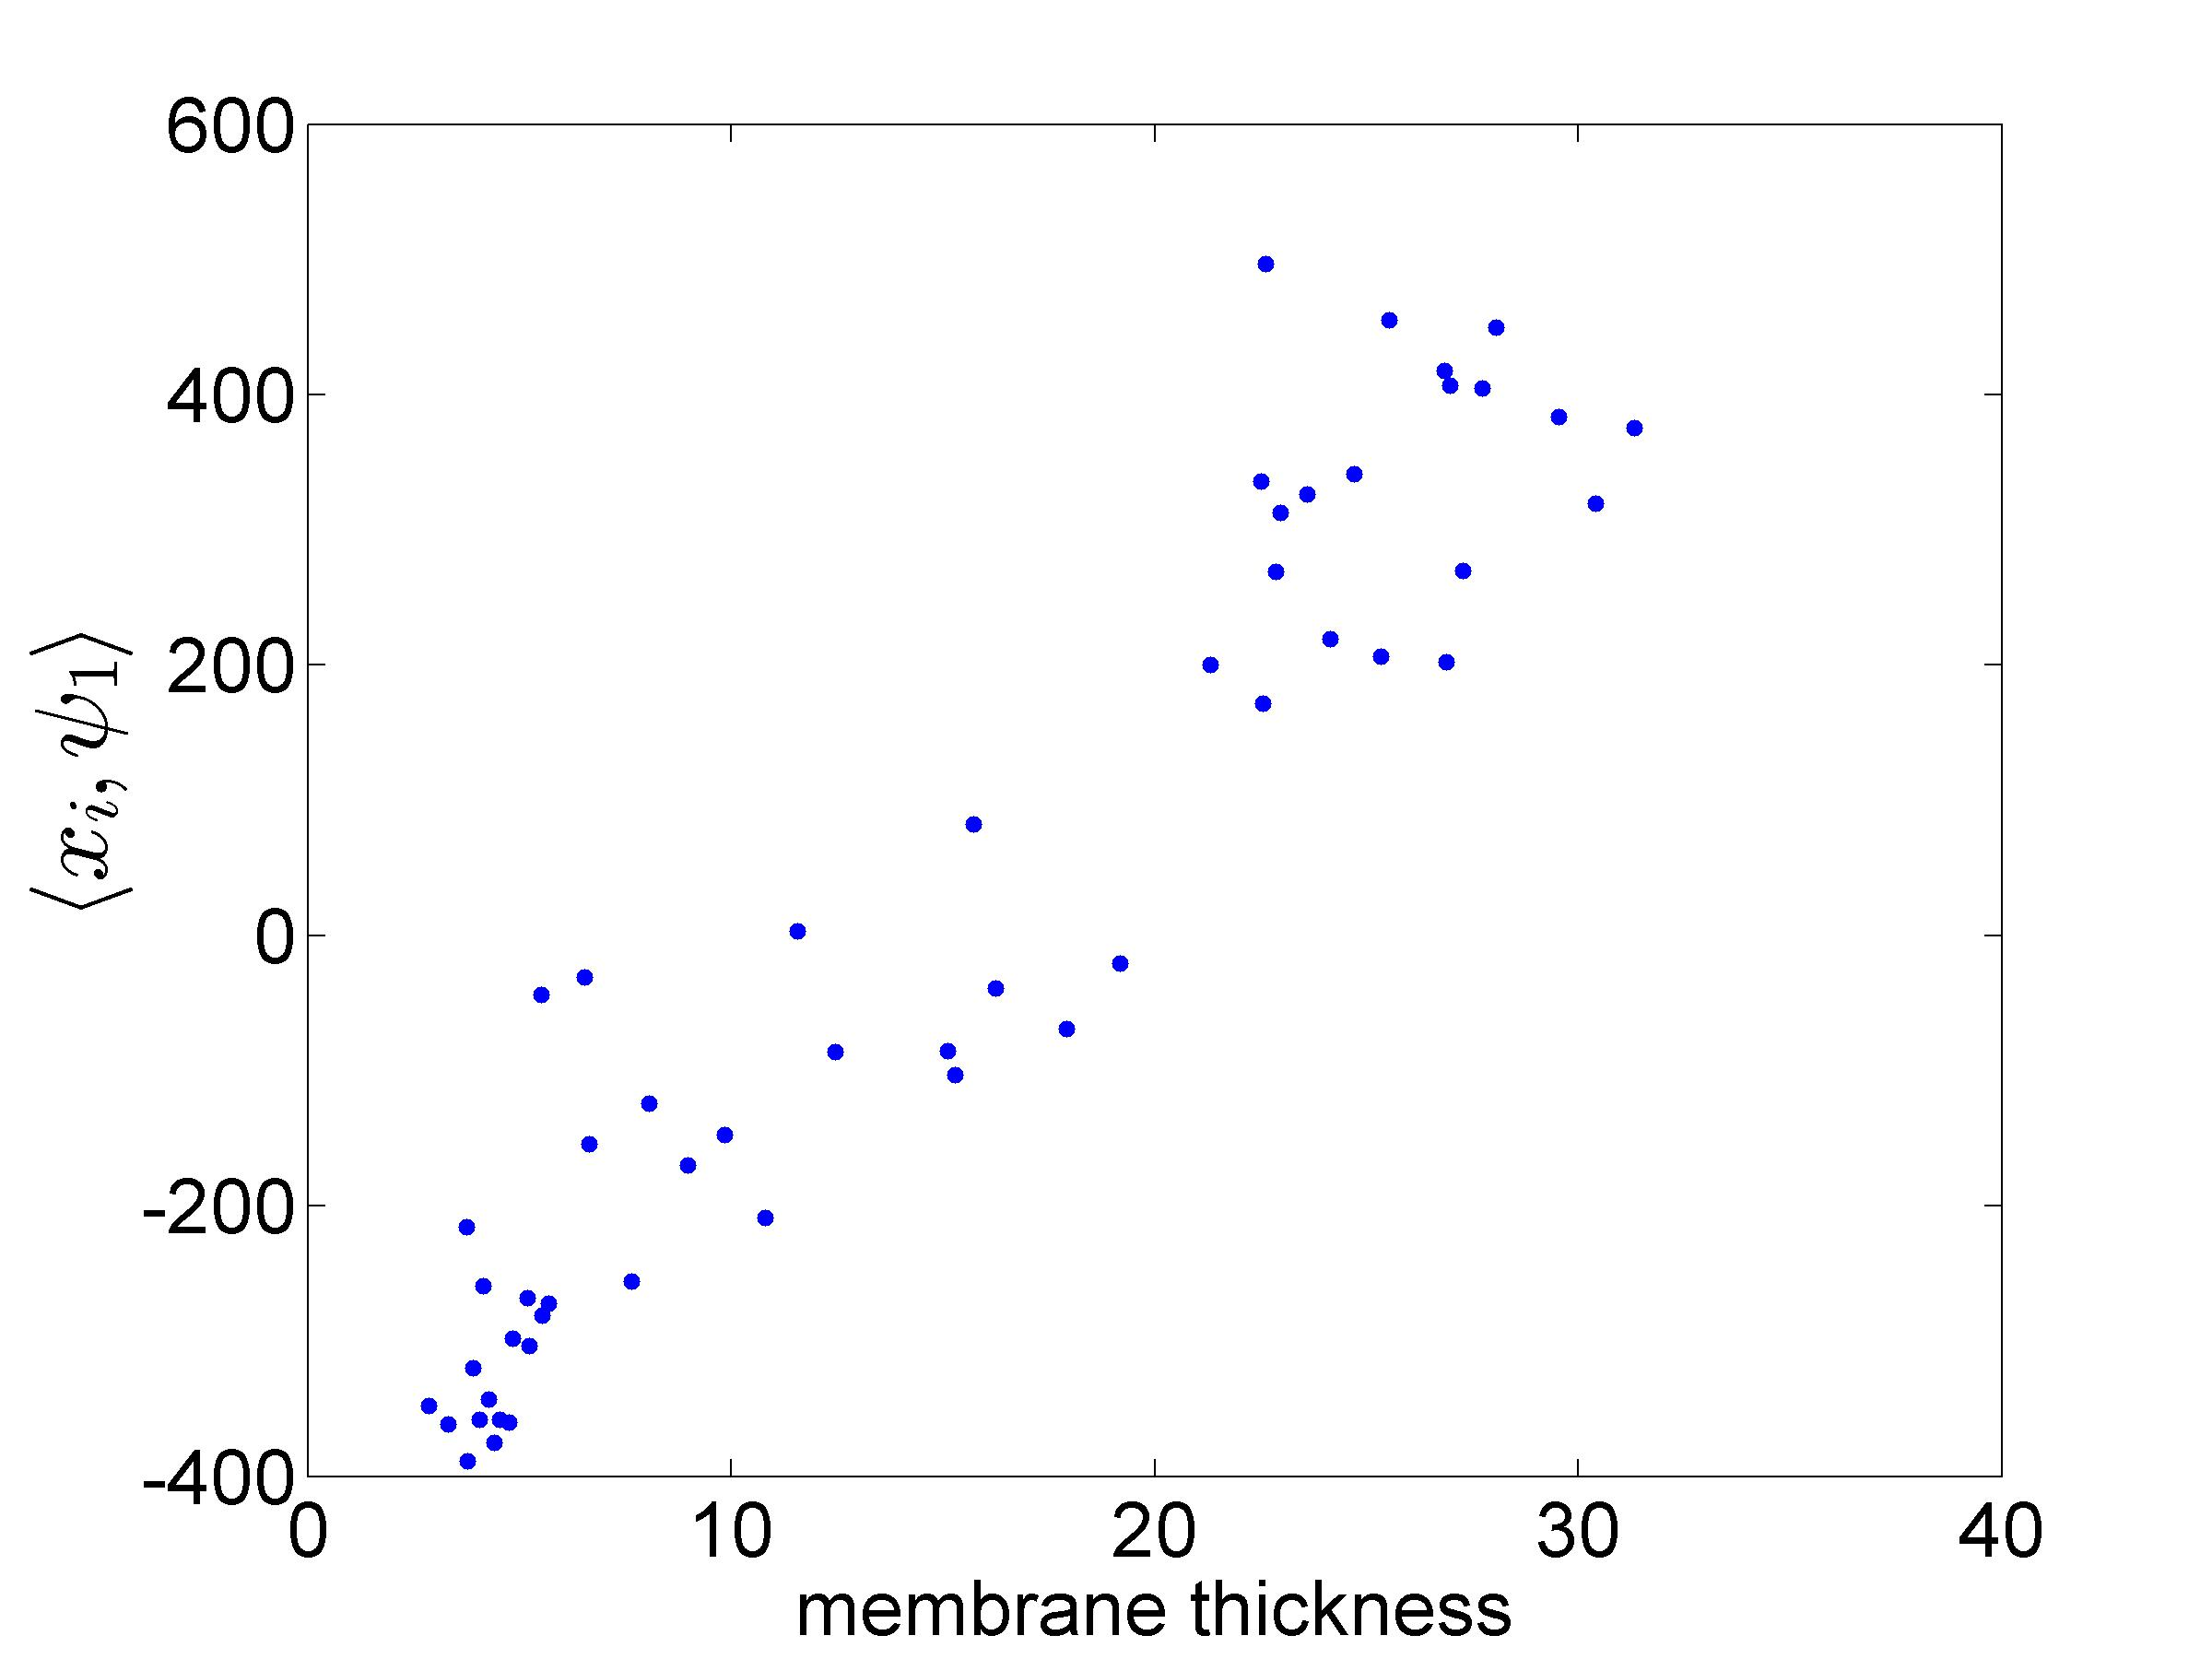
\includegraphics[width=\textwidth]{PCA_time_corr}
\caption{}
\end{subfigure}
\caption{{\bf Ordering dpERK concentration profiles using PCA.} (a) Concentration profiles of dpERK for many embryos. Each row represents a different embryo fixed at a slightly different developmental time.
(b) Concentration profiles of dpERK from (a), now ordered by the first PCA projection coefficient.
(c) Correlation between the first PCA projection coefficient and the membrane thickness.}
\label{fig:PCA_ordering}
\end{figure}

We would like to note that, because the embryos can be oriented with either the anterior or posterior facing up in the microfluidic device (see Figure \ref{subfig:imaging_device}), the directionality of the concentration profiles (clockwise versus counterclockwise around the ring, or right-to-left versus left-to-right for the linear profiles) is not meaningful. 
%
Therefore, we could do PCA with an expanded data set where we also include the mirror image of each concentration profile.
%
Symmetries in PCA have been studied extensively in previous work \cite{holmes1998turbulence}; it was shown that when mirror images are also included in the data set, the first PCA mode captures the symmetric portion of the variability, and the second mode captures the anti-symmetric portion.
%
We found that including the mirror images of each data point did not change our results significantly, since the first principal component computed using the original data set (not shown) is nearly symmetric with respect to left-right reflections.

\subsection*{dpERK concentration profiles ordered using diffusion maps}

Although PCA was rather successful in ordering the concentration profiles, there are some inconsistencies in the orderings.
%
Perhaps the most obvious feature to note is the scrambling of the secondary peaks located at the far left and right edges of the concentration profiles.
%TODO: add name of secondary peaks
%
It is known that these peaks arise later in the development of {\em Drosophila} \cite{...};
however, one can see in Figure \ref{subfig:PCA_ordering_image} that these secondary peaks are scrambled when the data is ordered using PCA.
%
We can gain insight into this ``scrambling'' by looking at the projection of the data onto the first two principal components, shown in Figure \ref{subfig:PCA_12}.
%
The data falls onto a one-dimensional {\em nonlinear} curve in this two-dimensional space, implying that nonlinear dimensionality reduction techniques may be more appropriate.

We chose to use diffusion maps (DMAPS) as our nonlinear dimensionality reduction technique.
%
We computed the diffusion maps embedding for our data set, using the Euclidean distance between concentration profiles as our distance metric.
%
We then ordered the data using the first (nontrivial) diffusion maps coordinate $\phi_2$. 
%
The results are shown in Figure \ref{fig:DMAPS_ordering}; the Spearman correlation between $\phi_2$ and the membrane thickness is 0.9209.
%
The secondary peaks are now nicely clustered towards the end of the developmental trajectory.

\begin{figure}[!ht]
\begin{subfigure}{0.3\textwidth}
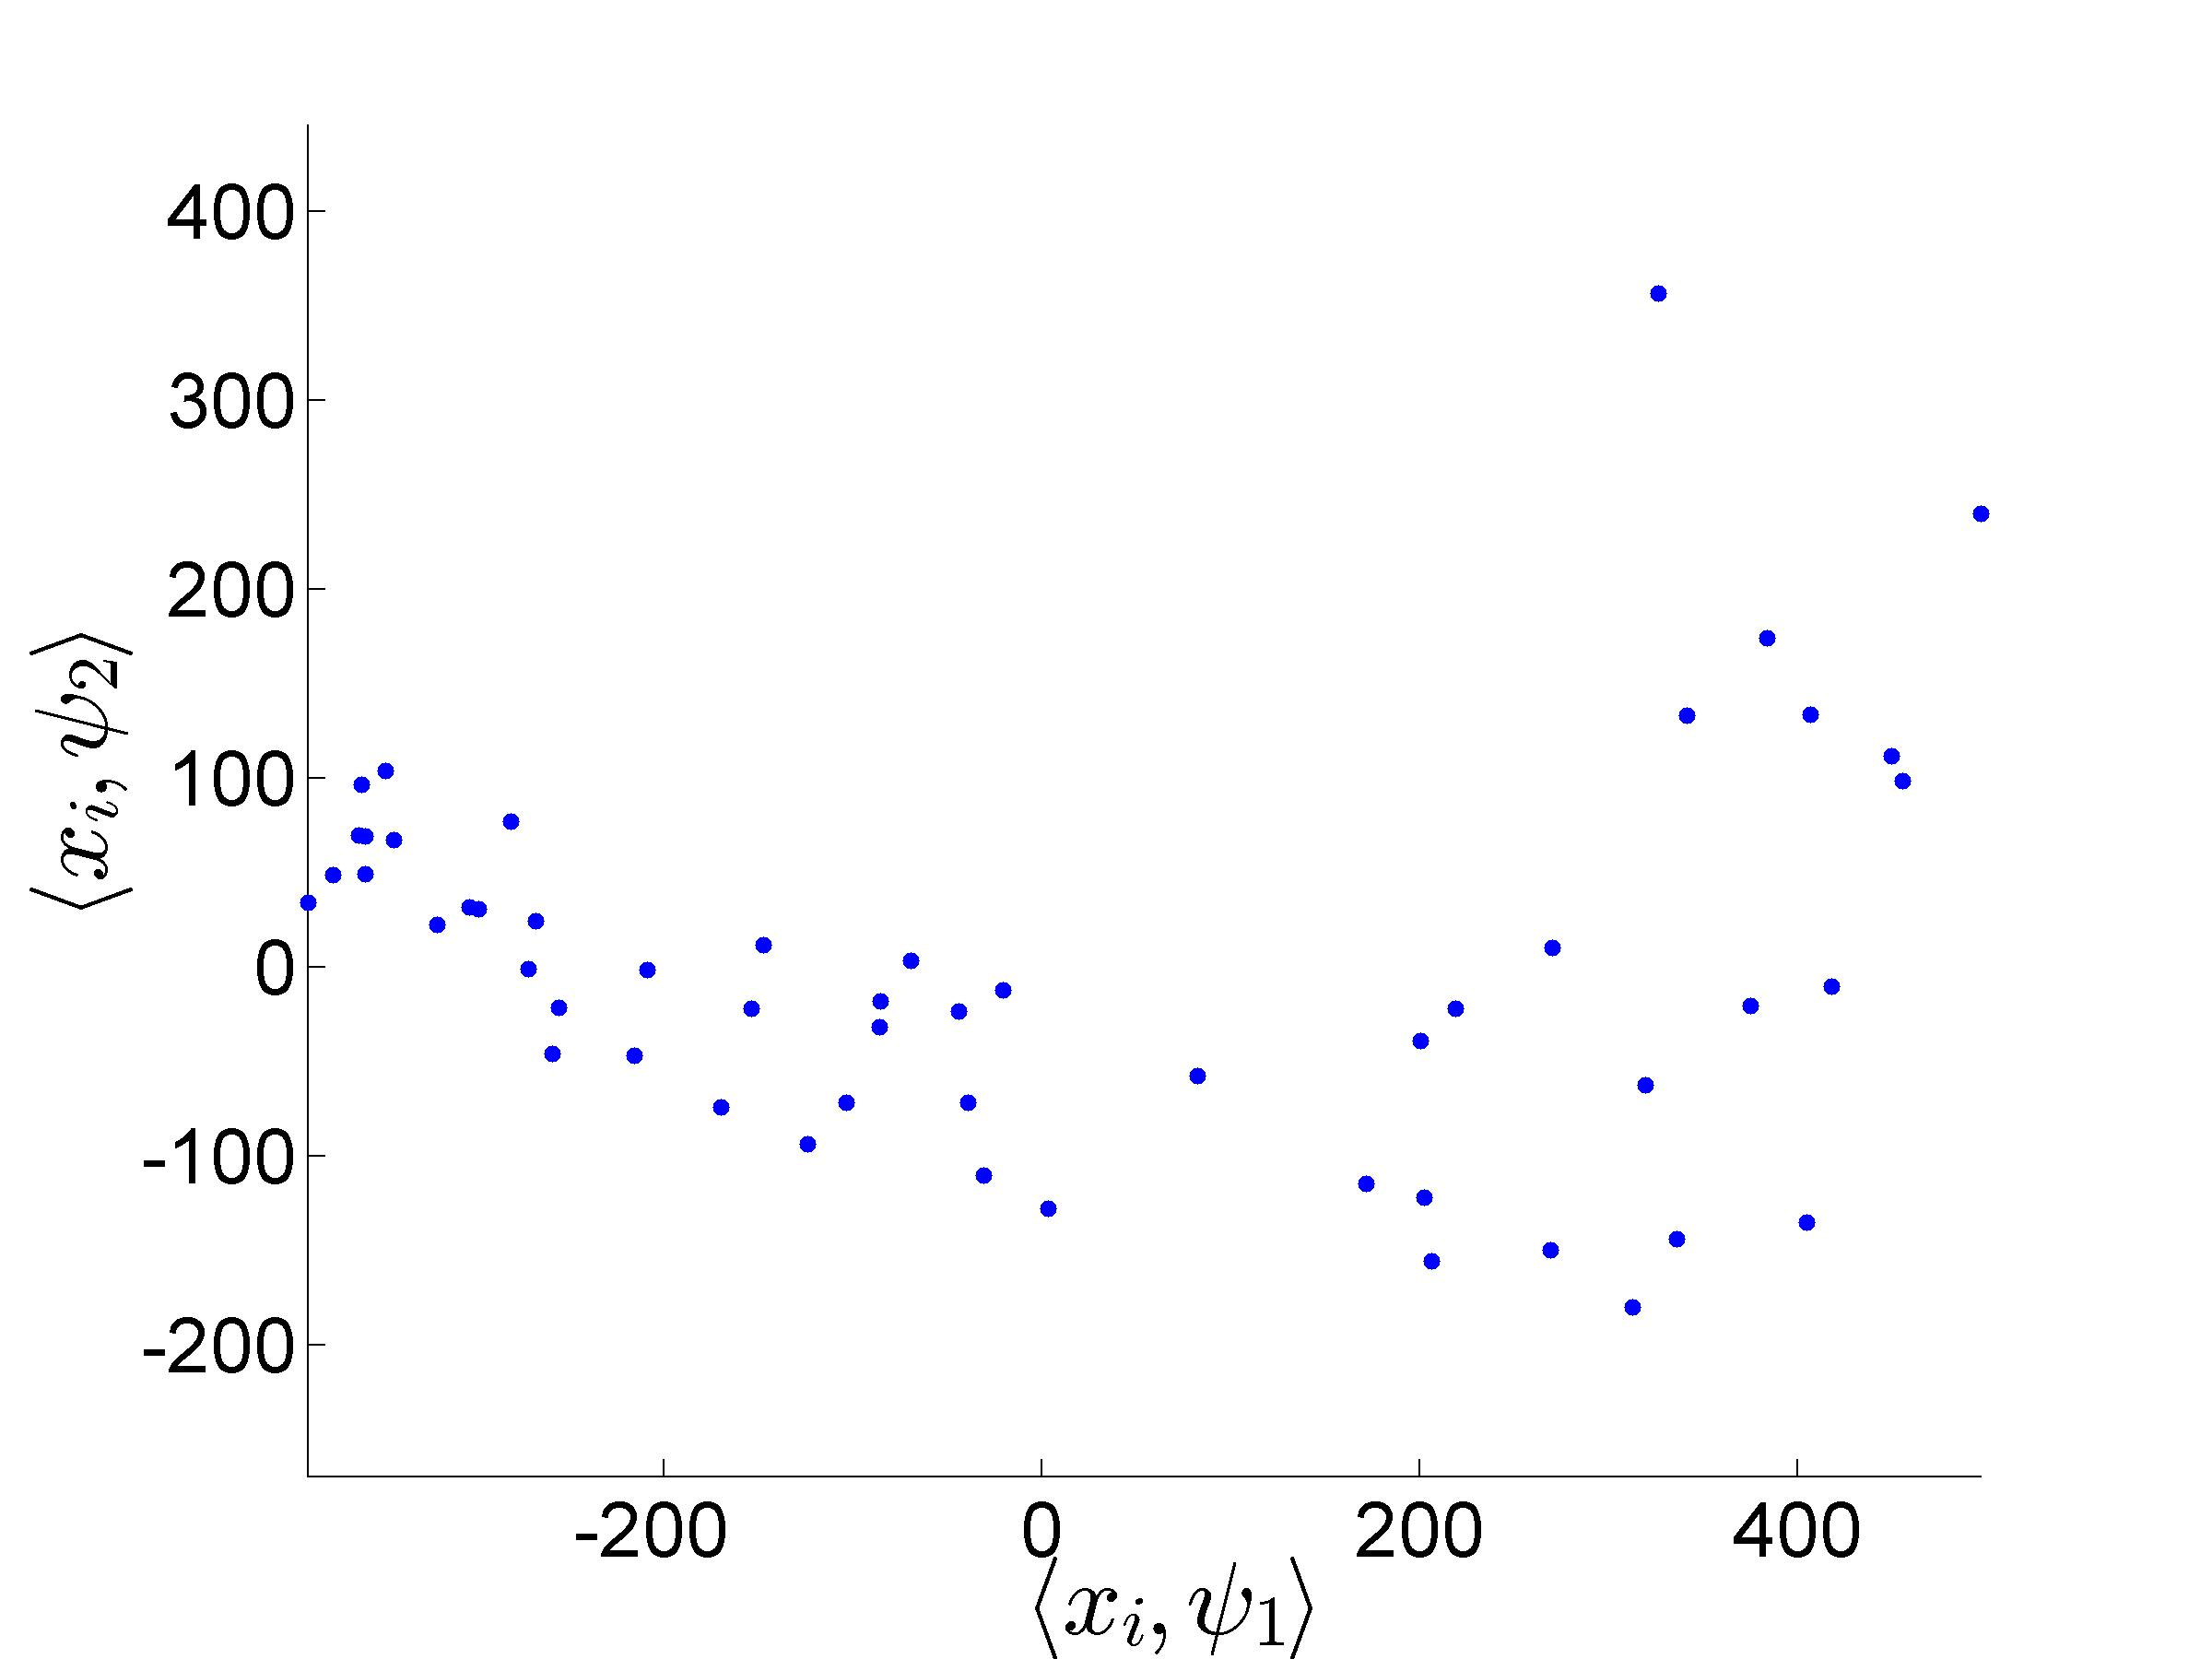
\includegraphics[width=\textwidth]{coeff_12_new}
\caption{}
\label{subfig:PCA_12}
\end{subfigure}
\begin{subfigure}{0.3\textwidth}
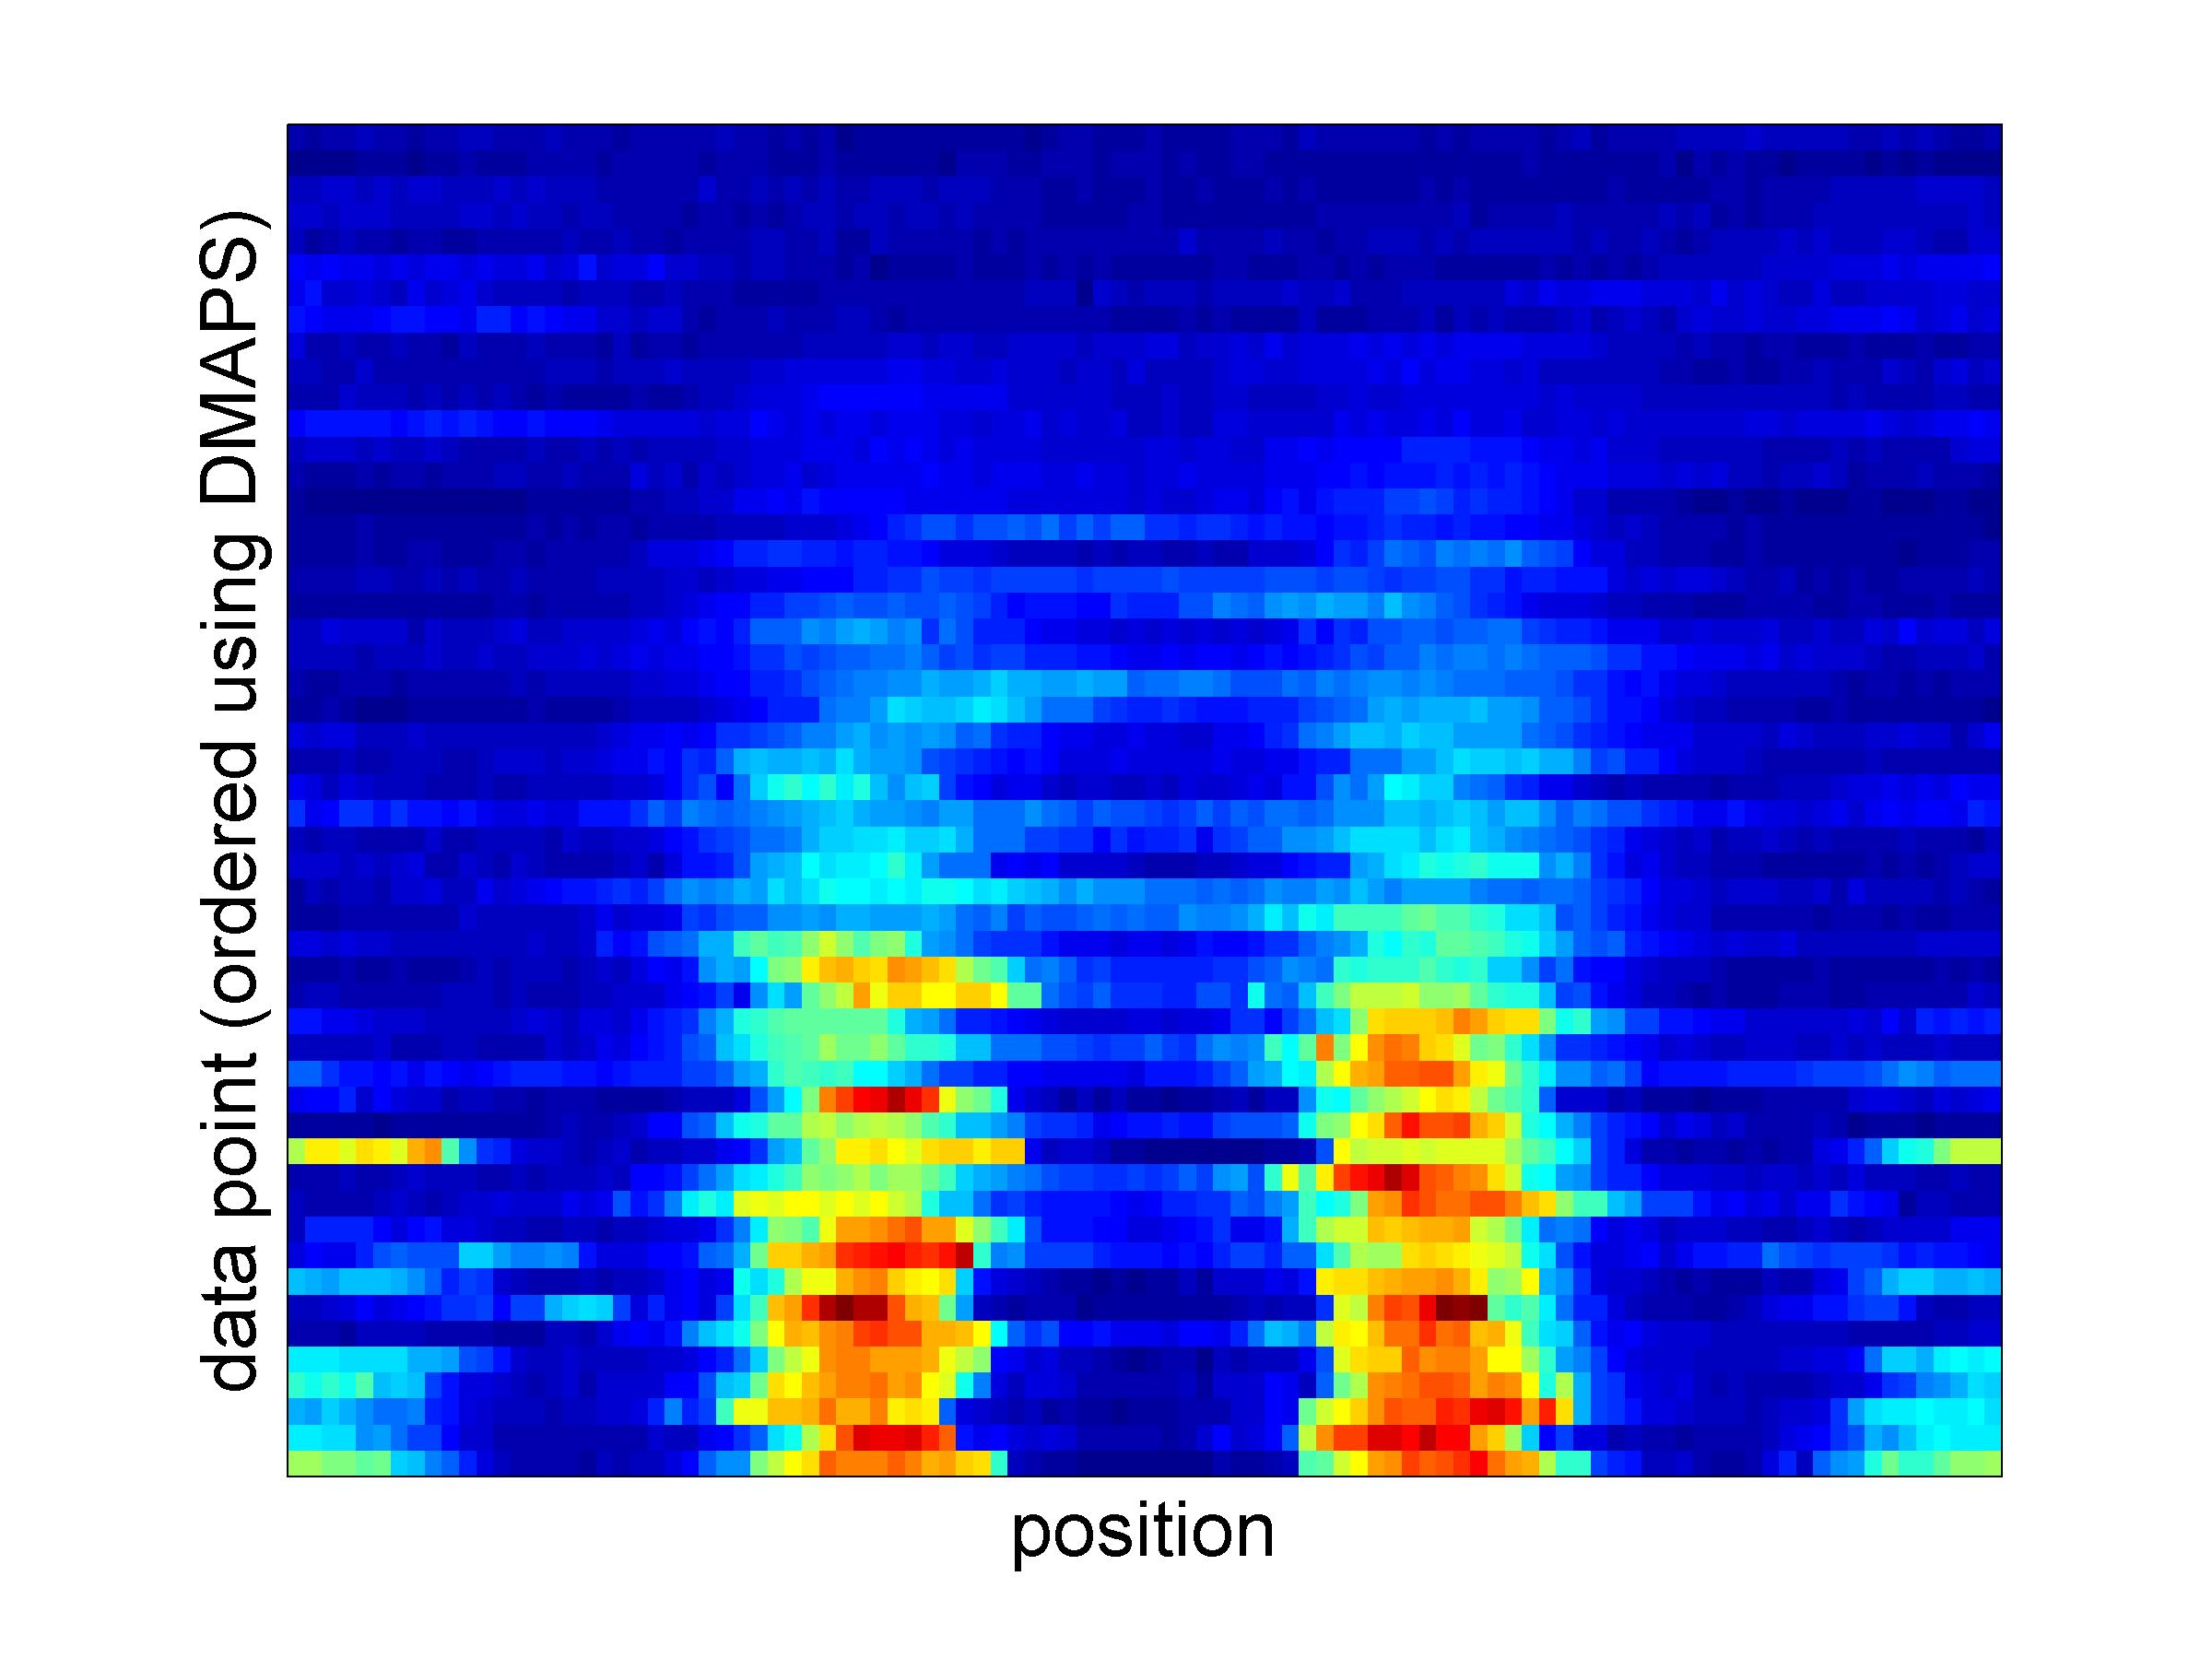
\includegraphics[width=\textwidth]{data_ordered_DMAPS}
\caption{}
\end{subfigure}
\begin{subfigure}{0.3\textwidth}
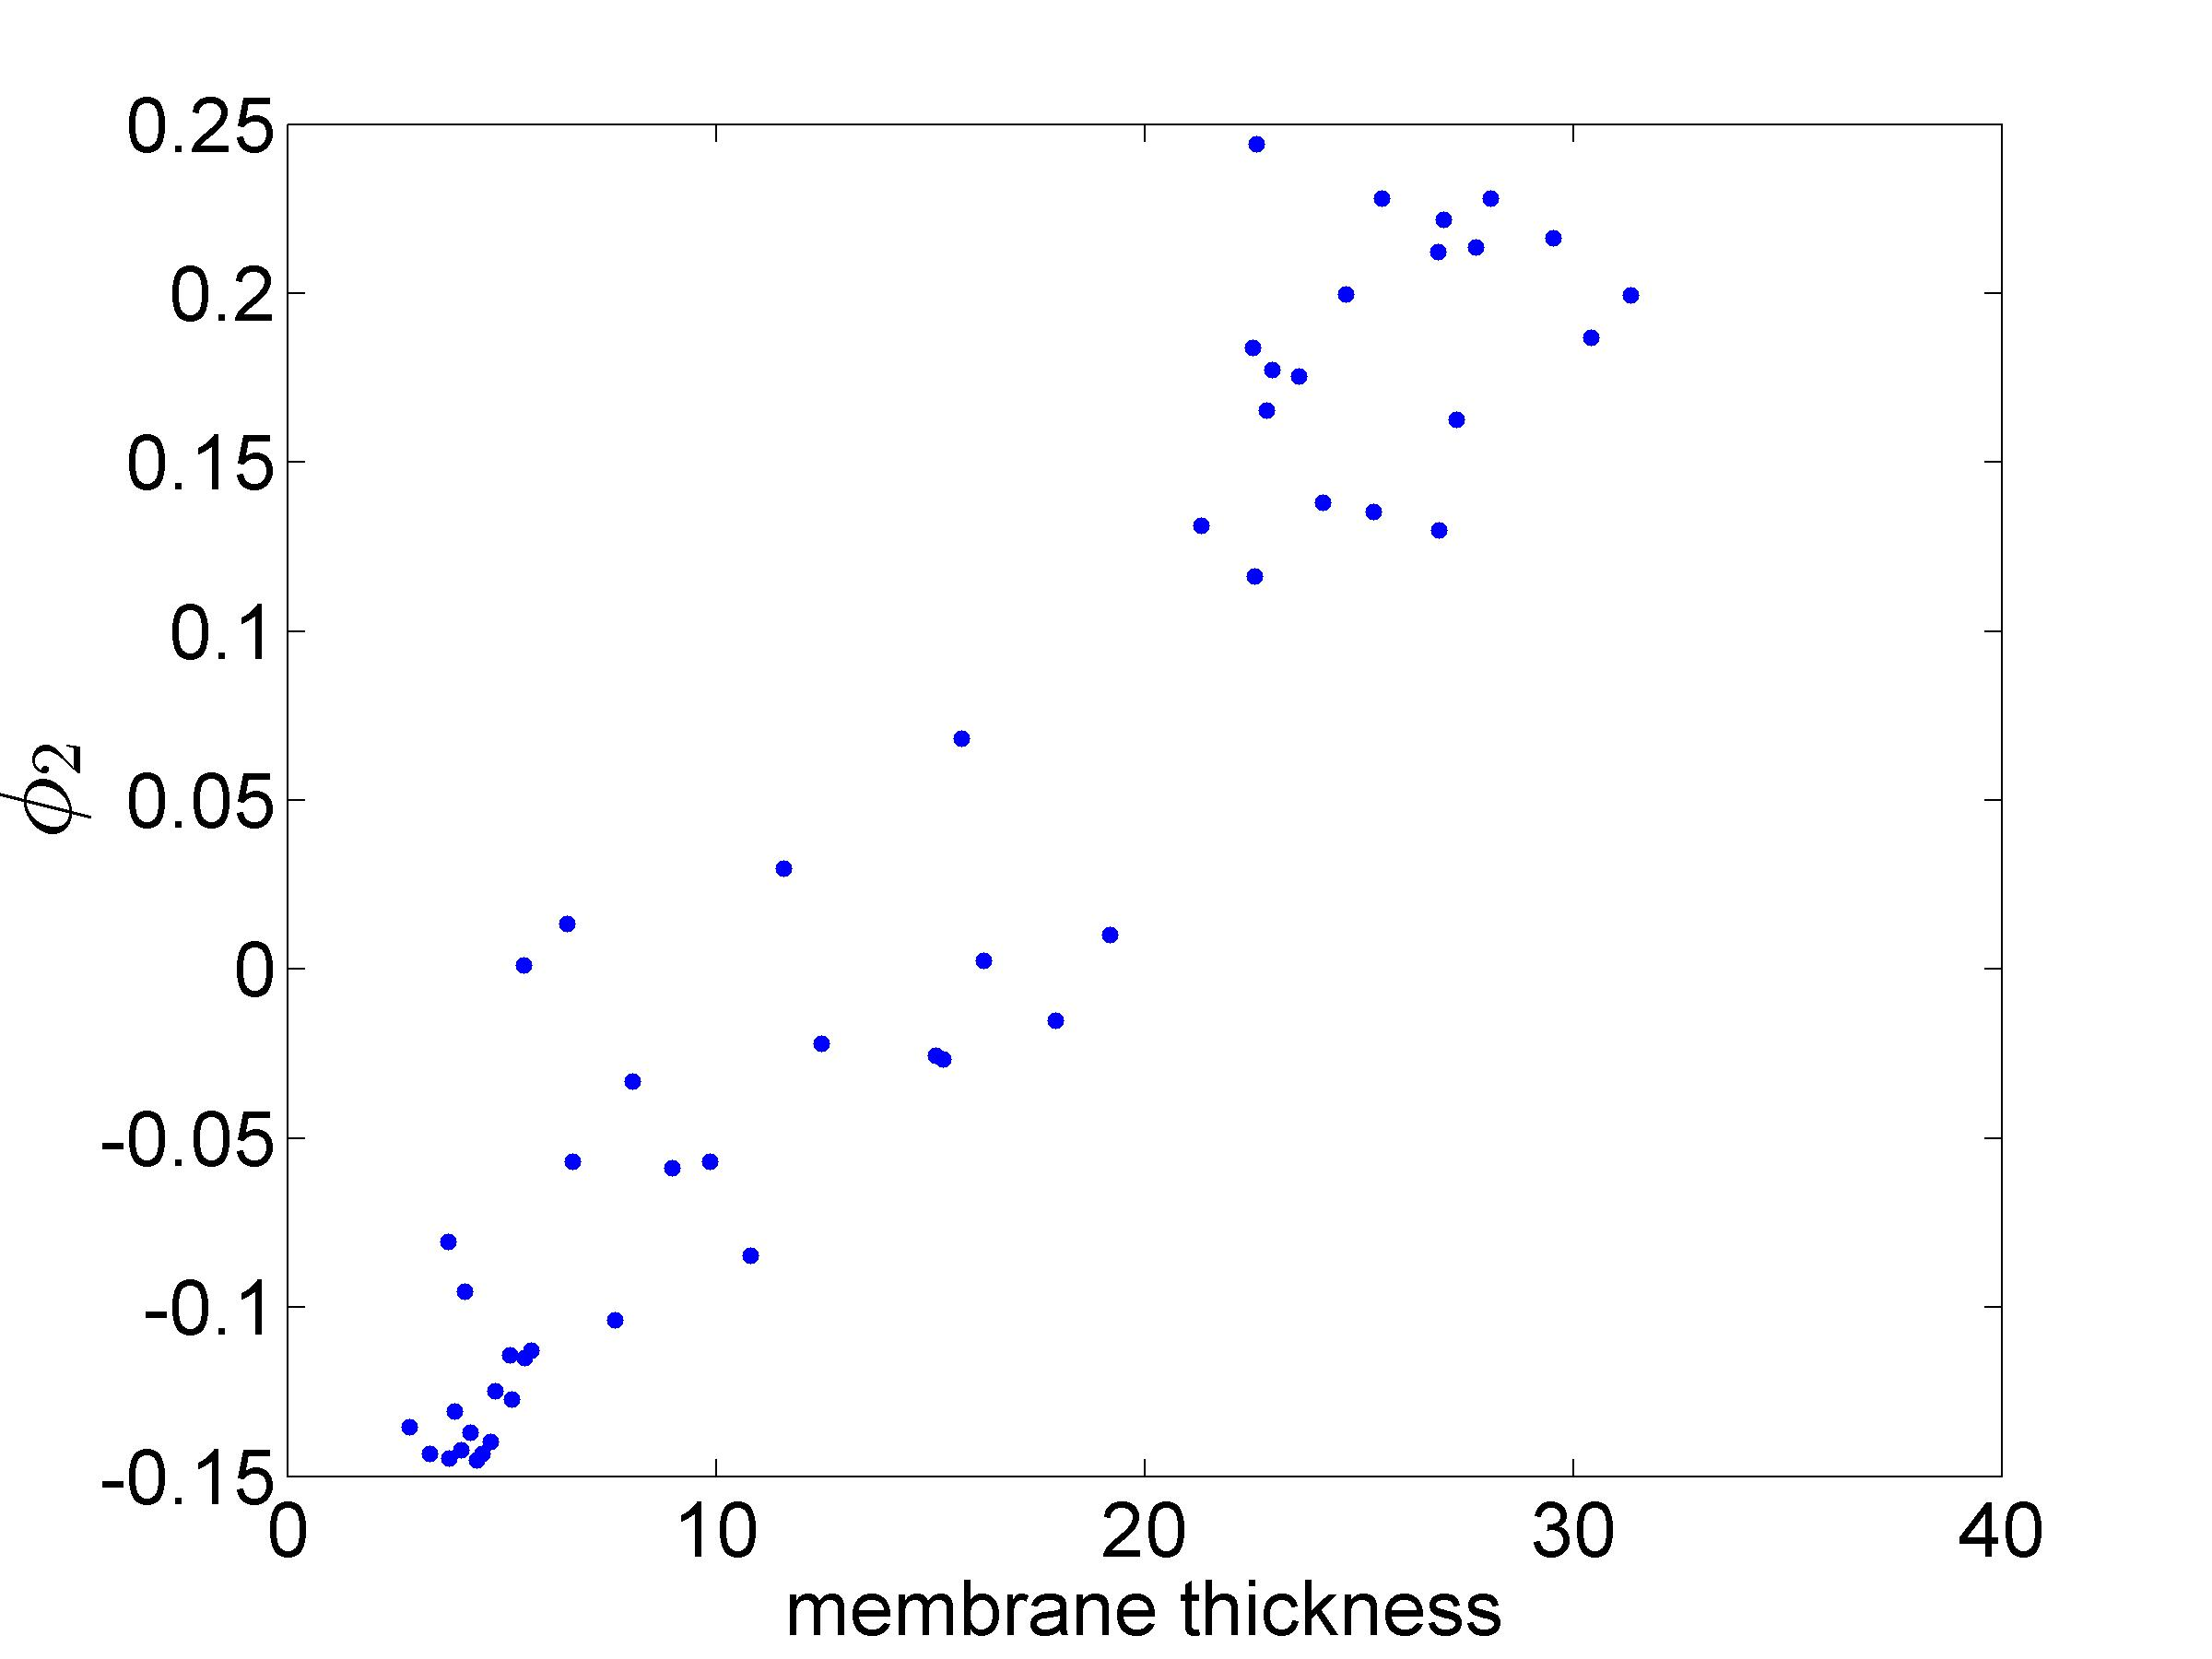
\includegraphics[width=\textwidth]{DMAPS_time_corr}
\caption{}
\end{subfigure}
\caption{{\bf Ordering dpERK concentration profiles using DMAPS.} (a) Projection of data shown in Figure \ref{subfig:unordered_profiles} onto the first two principal components; note that the data falls on an (effectively) one-dimensional, nonlinear curve. 
(b) Concentration profiles of dpERK from (a), now ordered by the first non-trivial DMAPS embedding coordinate.
(c) Correlation between the first (non-trivial) DMAPS embedding coordinate and the membrane thickness.}
\label{fig:DMAPS_ordering}
\end{figure}

\subsection*{dpERK concentration profiles aligned using angular synchronization}

We have demonstrated that we can order the concentration profiles using PCA or DMAPS.
%
However, ordering the profiles first requires that we factor out the relevant symmetries in the problem.
%
The developmental dynamics are invariant to the orientation of the embryo in the microfluidic device; therefore, to obtain meaningful results from our analysis, we must first align the concentration profiles.
%
Rotations of the embryo cross-sections correspond to translations (with periodic boundary conditions) of the linear profiles we have been studying.
%
In the previous analyses, we have assumed that the profiles have been prealigned using the location of the dorsal protein peak.
%
However, without some {\em a priori} knowledge of the system (e.g. without knowing that dorsal is expressed at one position along the perimeter of the embryo), we would need to align the concentration profiles before doing our analysis.
%TODO: add when this might be relevant, e.g. when there is no Dorsal

The most common and perhaps intuitive techniques for alignment are template-based methods \cite{ahuja2007template}, where one chooses are representative data point or shape as a ``template'', and then shifts or rotates each data point to be optimally aligned with this template.
%
Although these methods are simple, they require knowledge of an appropriate template function and can suffer when the data set is noisy \cite{sonday2013noisy}.
%
Angular synchronization \cite{singer2011angular} is a relatively new technique that is often more robust than template-based methods in the presence of noise.
%
We used angular synchronization to factor out the shifts and align the concentration profiles measured from the fluorescent images.
%
Because the concentration profiles lie on a circle (we unwrap them onto a line for visualization purposes), factoring out shifts of the linear profiles (with periodic boundary conditions) corresponds to factoring out rotations of a circle with the underlying symmetry group $SO(2)$. 
%
After alignment, we used DMAPS to order the aligned concentration profiles.
%
The results are shown in Figure \ref{fig:angsynch_ordering}.
%
One can see that the results are visually consistent with the results shown in Figure \ref{fig:DMAPS_ordering}; the Spearman correlation between $\phi_2$ and the membrane length is 0.9164. 

\begin{figure}[!ht]
\begin{subfigure}{0.3\textwidth}
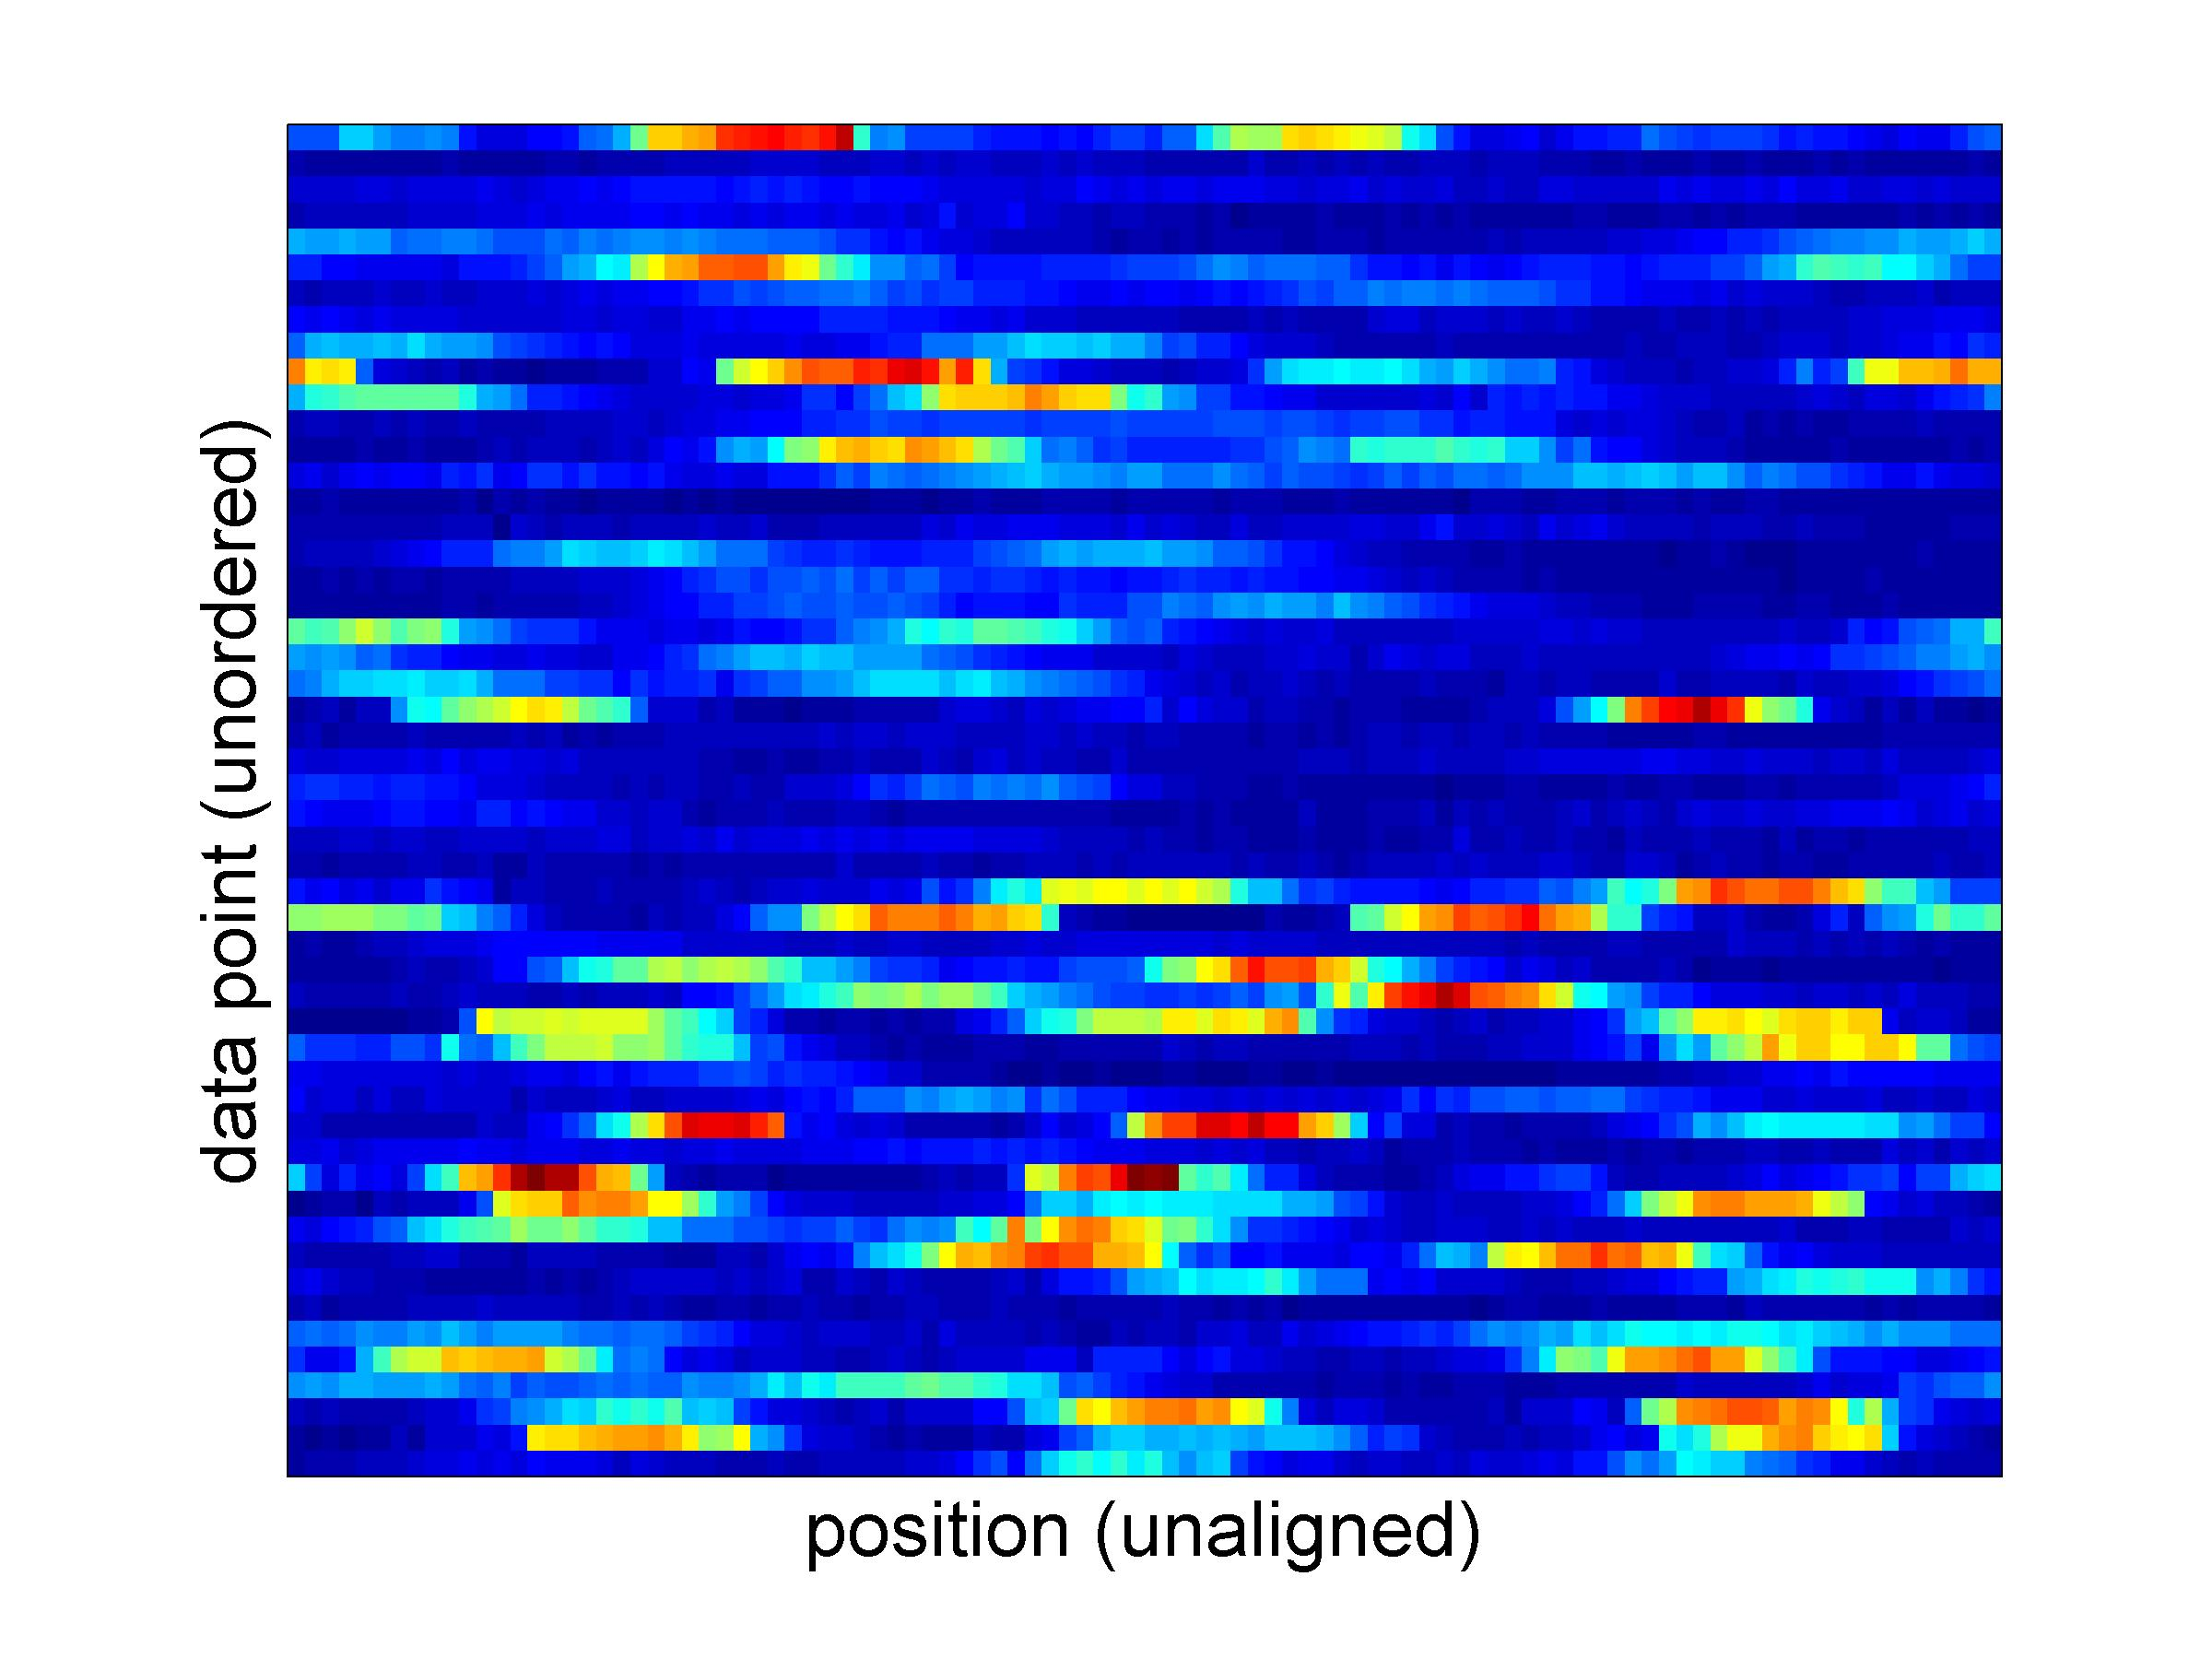
\includegraphics[width=\textwidth]{data_unaligned_unordered}
\caption{}
\end{subfigure}
\begin{subfigure}{0.3\textwidth}
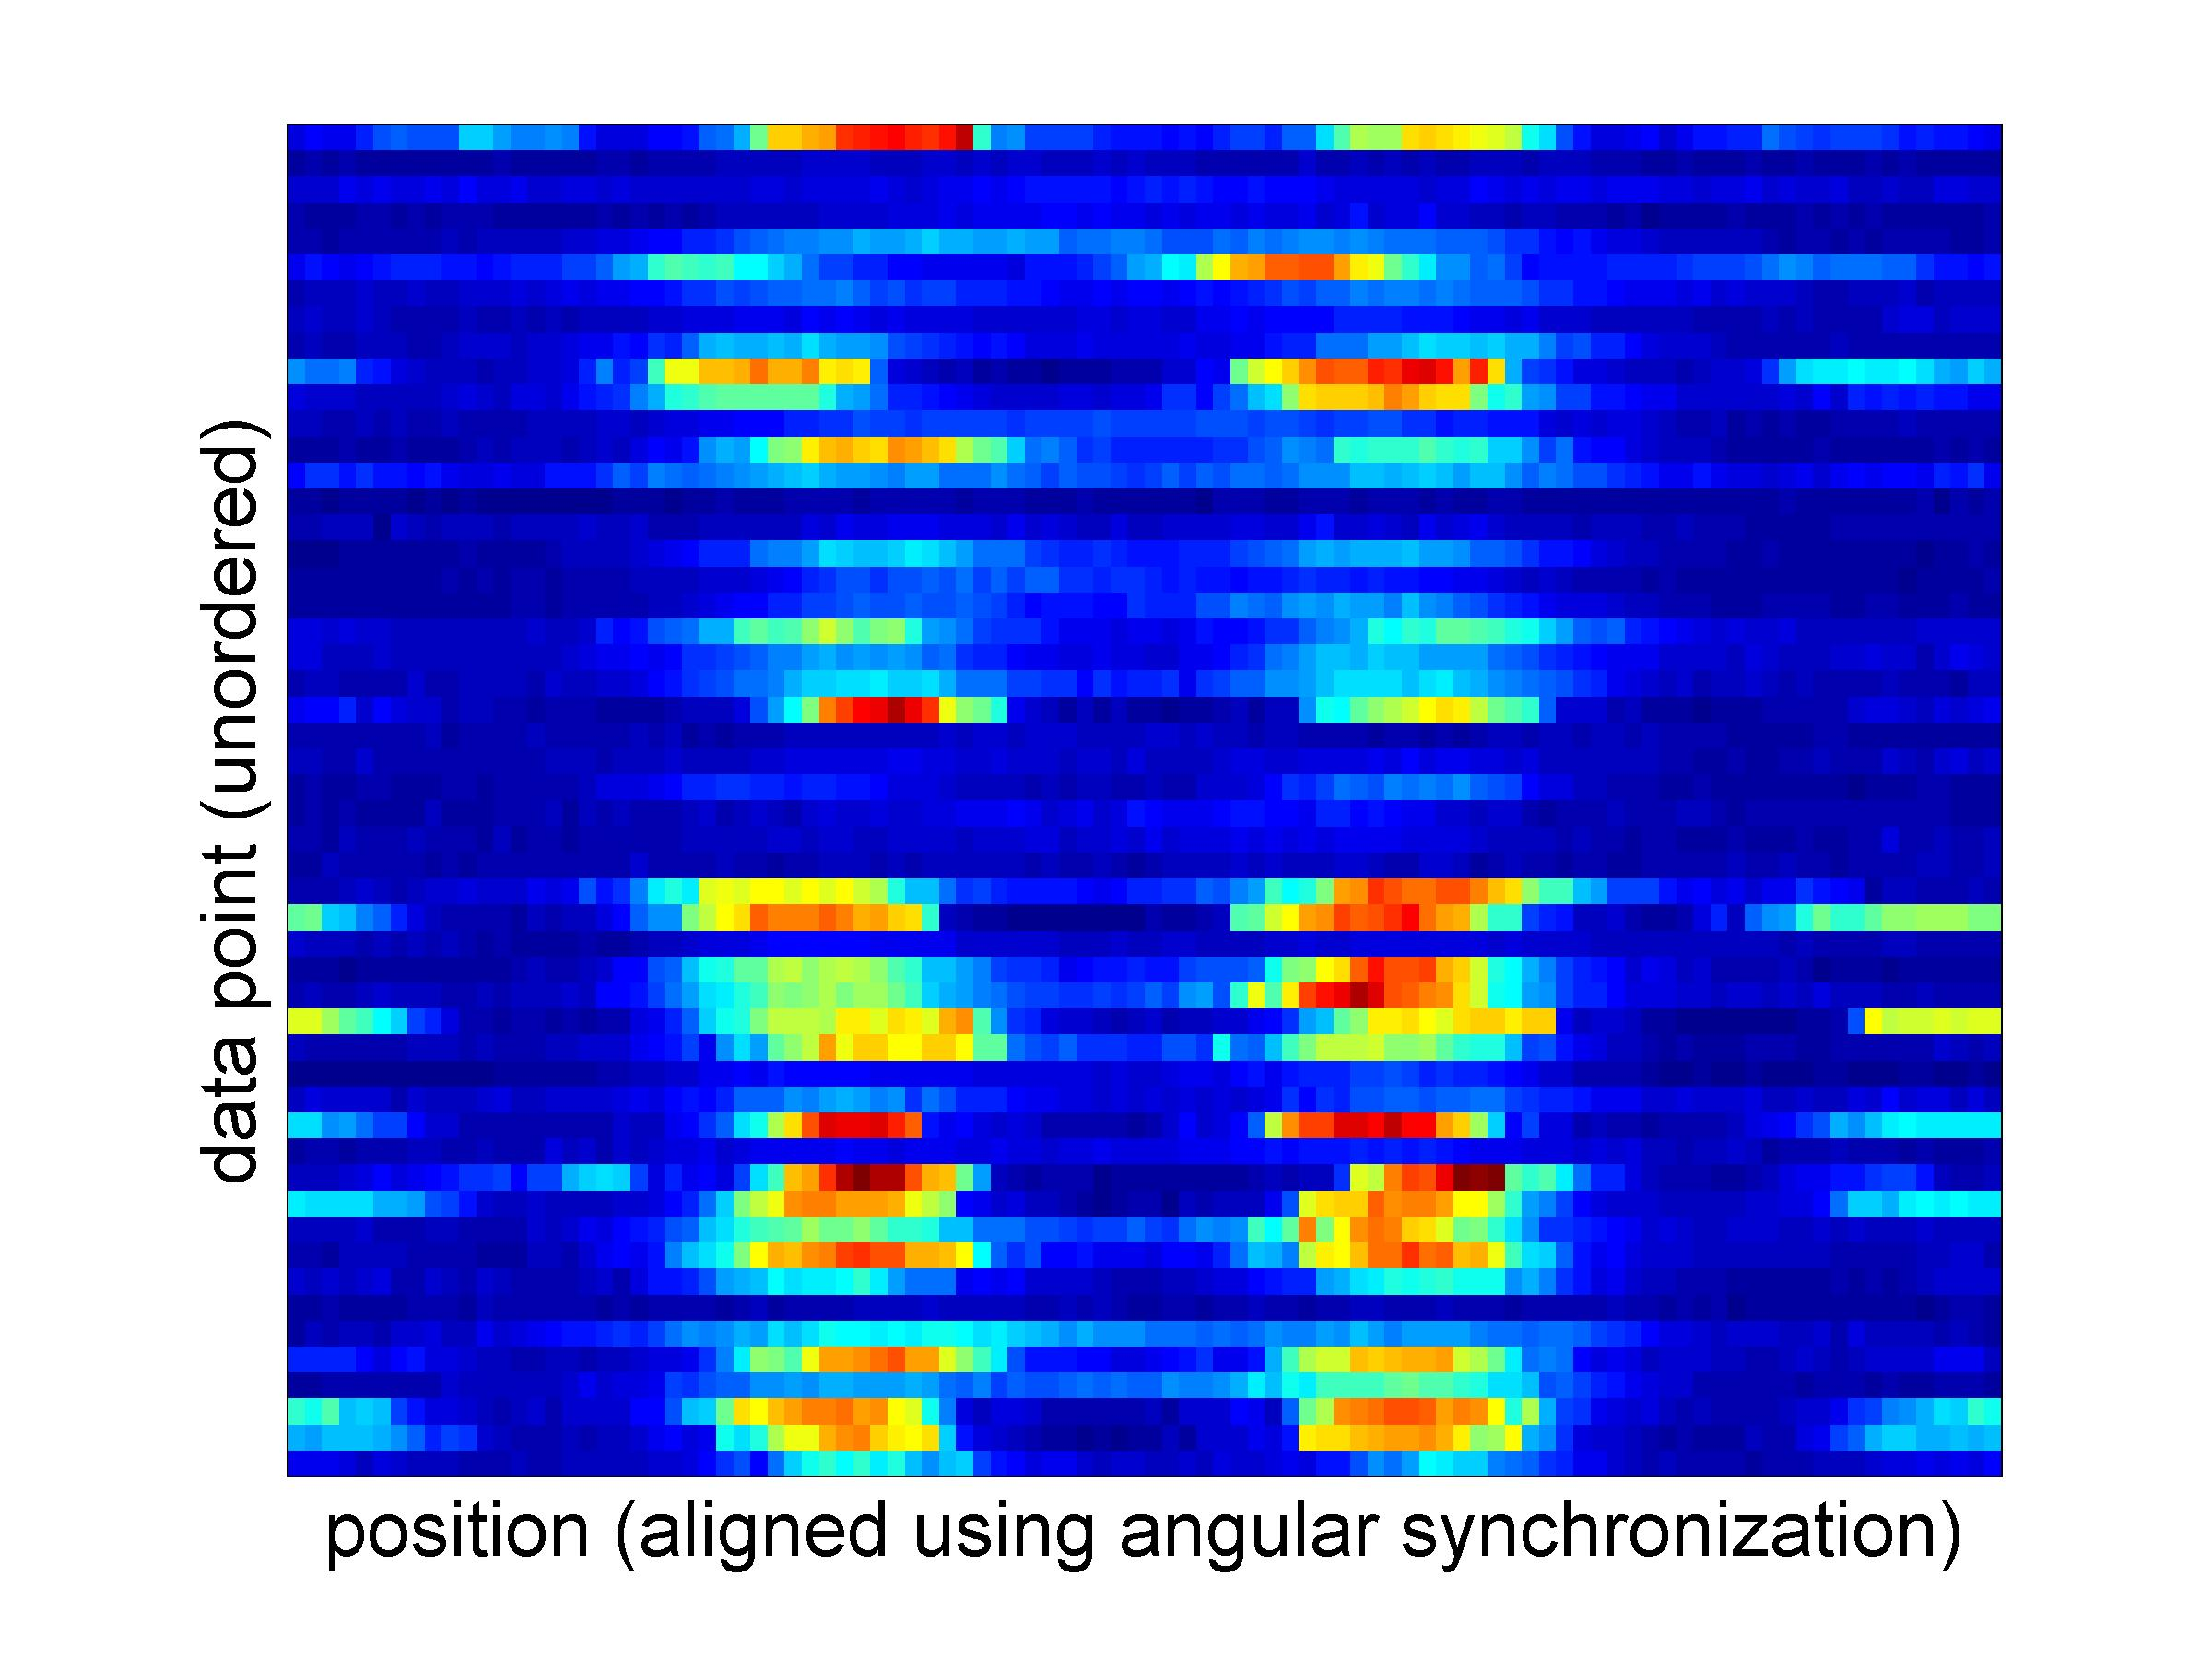
\includegraphics[width=\textwidth]{data_aligned_unordered}
\caption{}
\end{subfigure}
\begin{subfigure}{0.3\textwidth}
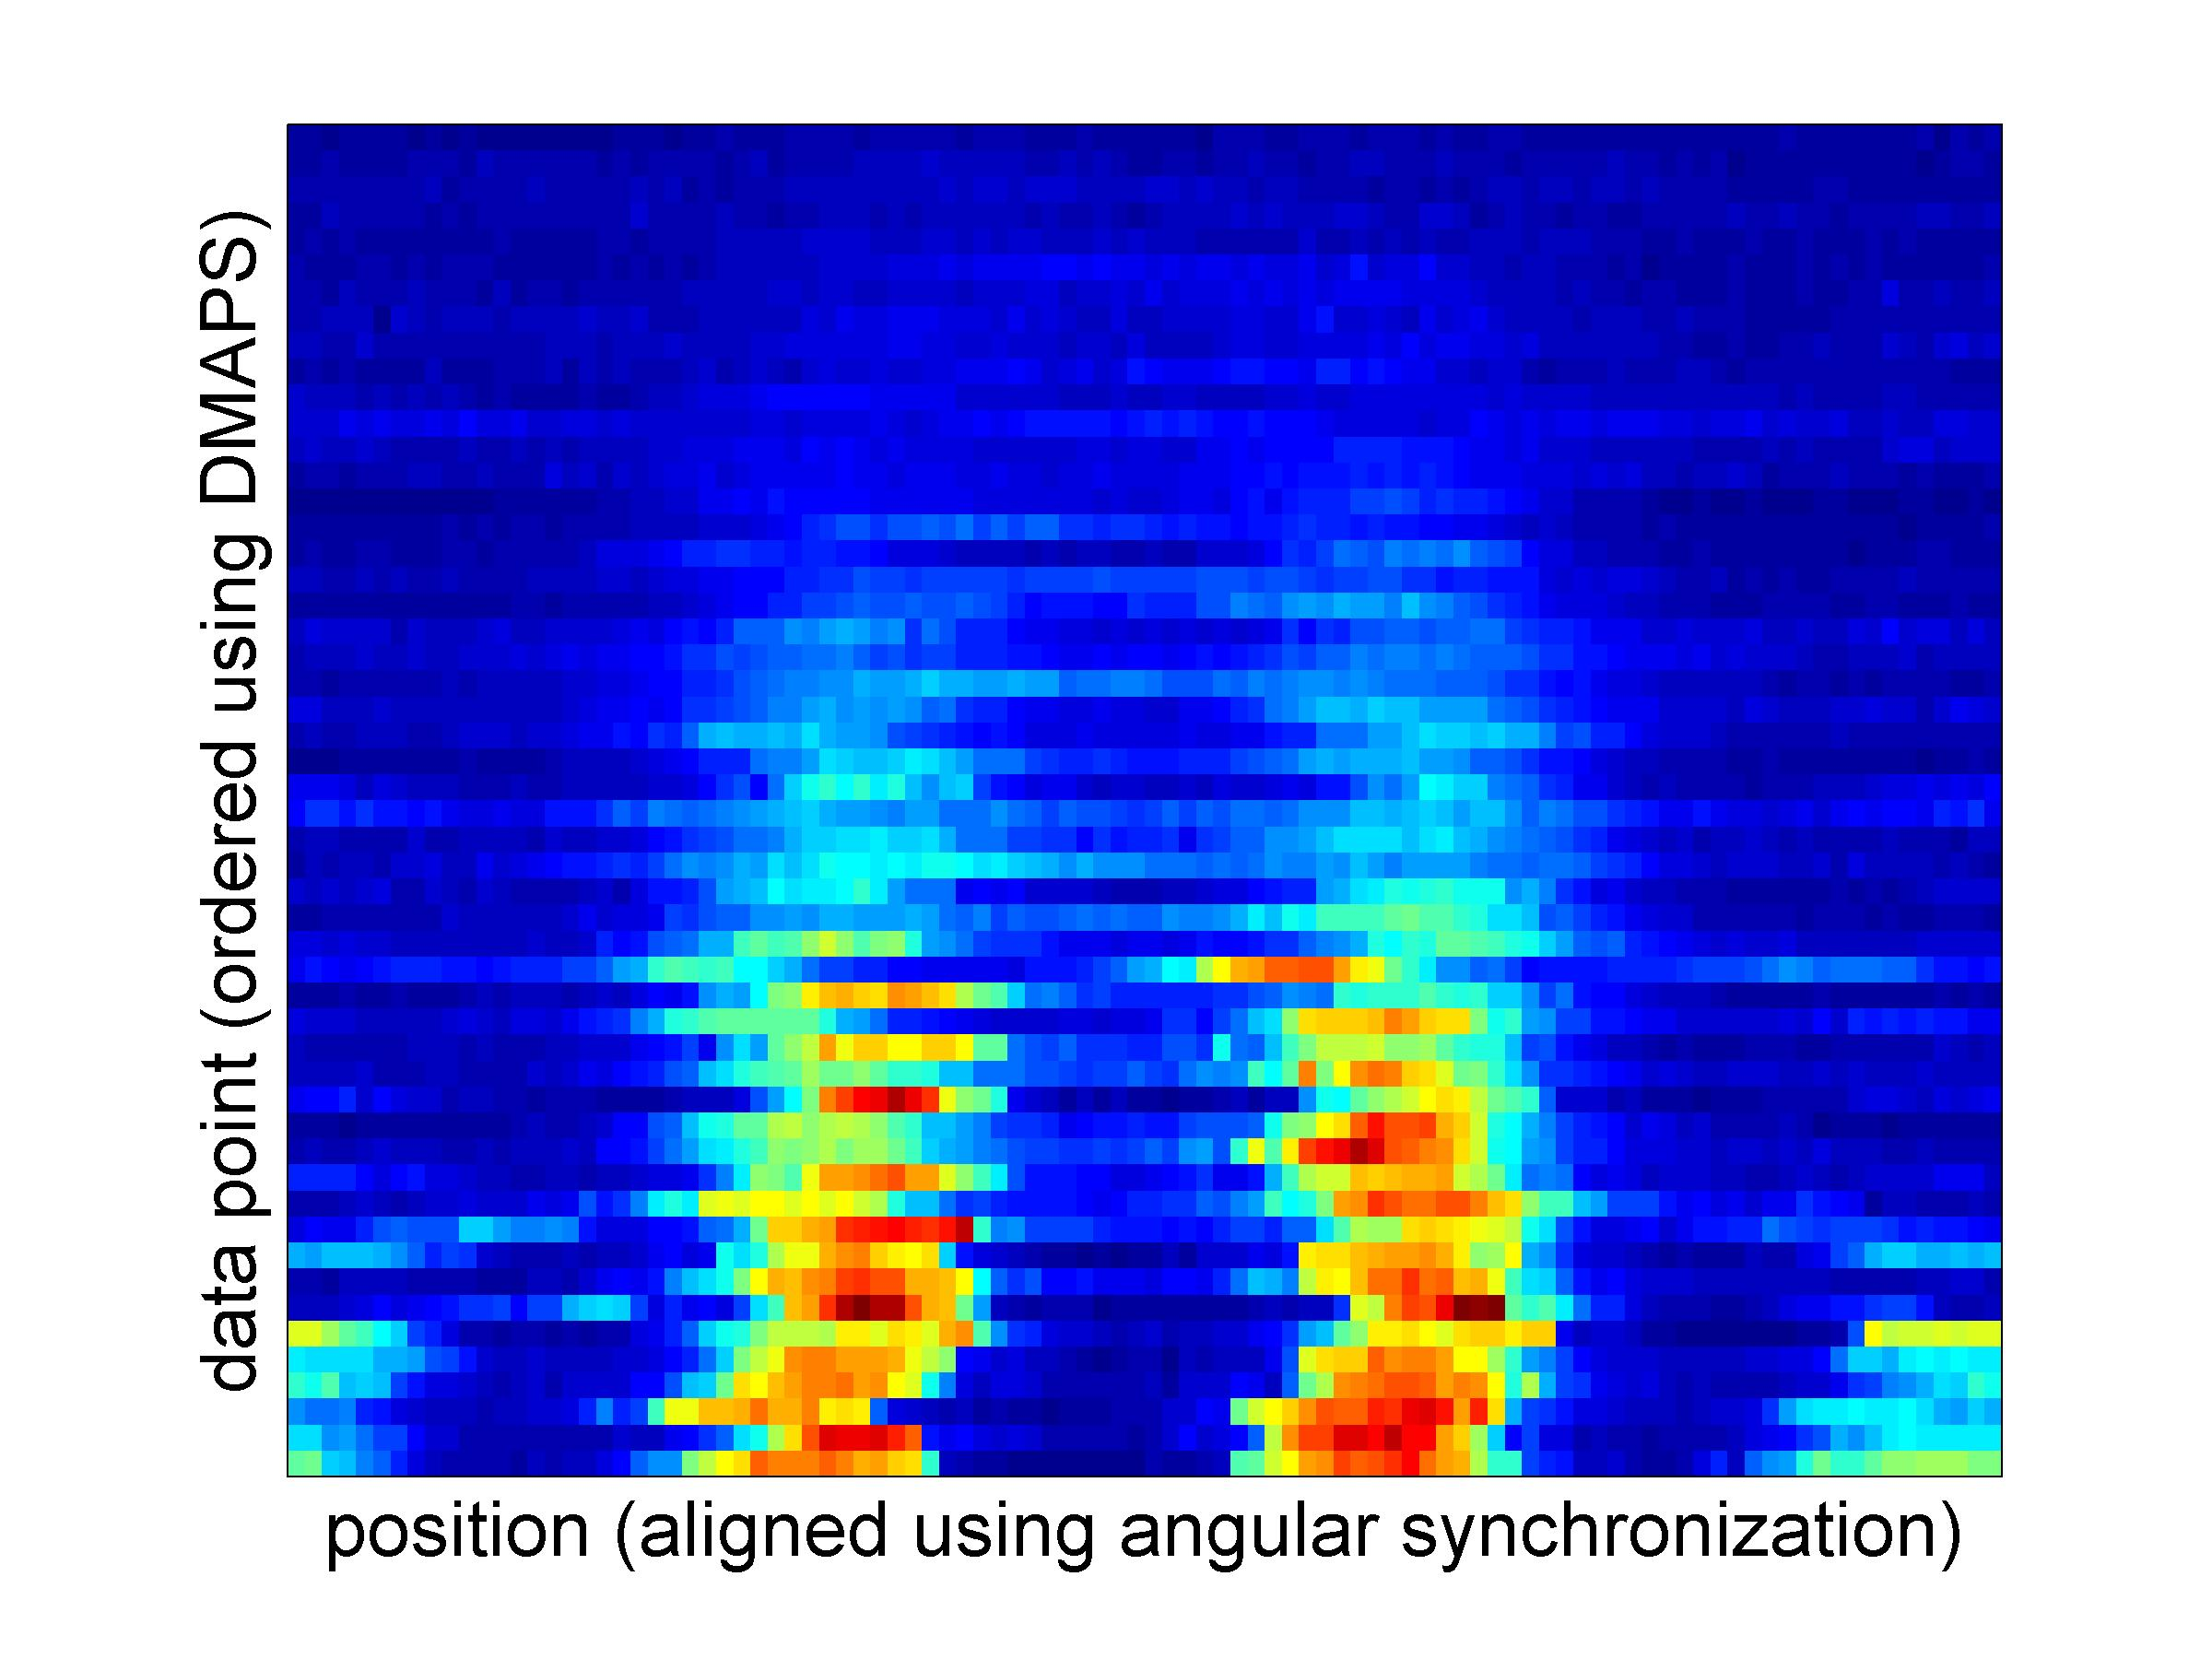
\includegraphics[width=\textwidth]{data_ordered_angsynch}
\caption{}
\end{subfigure}
\caption{{\bf Ordering spatially unaligned dpERK concentration profiles.} (a) Concentration profiles of dpERK for many embryos. Each row represents a different embryo fixed at a slightly different developmental time. The circluar profiles have not been ``opened'' at the same point; rather, each profile was opened at a random point around the embryo. We are allowed to shift the (linear) profiles left and right.
(b) Concentration profiles of dpERK aligned using angular synchronization.
(c) Concentration profiles of dpERK aligned using angular synchronization and ordered by the first (non-trivial) DMAPS embedding coordinate.}
\label{fig:angsynch_ordering}
\end{figure}

\subsection*{dpERK concentration profiles aligned and ordered using vector diffusion maps}

Instead of using angular synchronization followed by DMAPS, one can do the alignment and ordering in one computation using vector diffusion maps (VDM).
%
VDM is similar to angular synchronization, but it operates on data sets that contain both underlying symmetries and dynamics.
%
The results of aligning {\em and} ordering the data using VDM are shown in Figure \ref{fig:vdm_ordering}; the results are similar to those from angular syncrhonization (Figure \ref{fig:angsynch_ordering}), and the Spearman correlation between $\langle \phi_3, \phi_1 \rangle$ and the membrane length is 0.9123.

\begin{figure}[!ht]
\begin{subfigure}{0.3\textwidth}
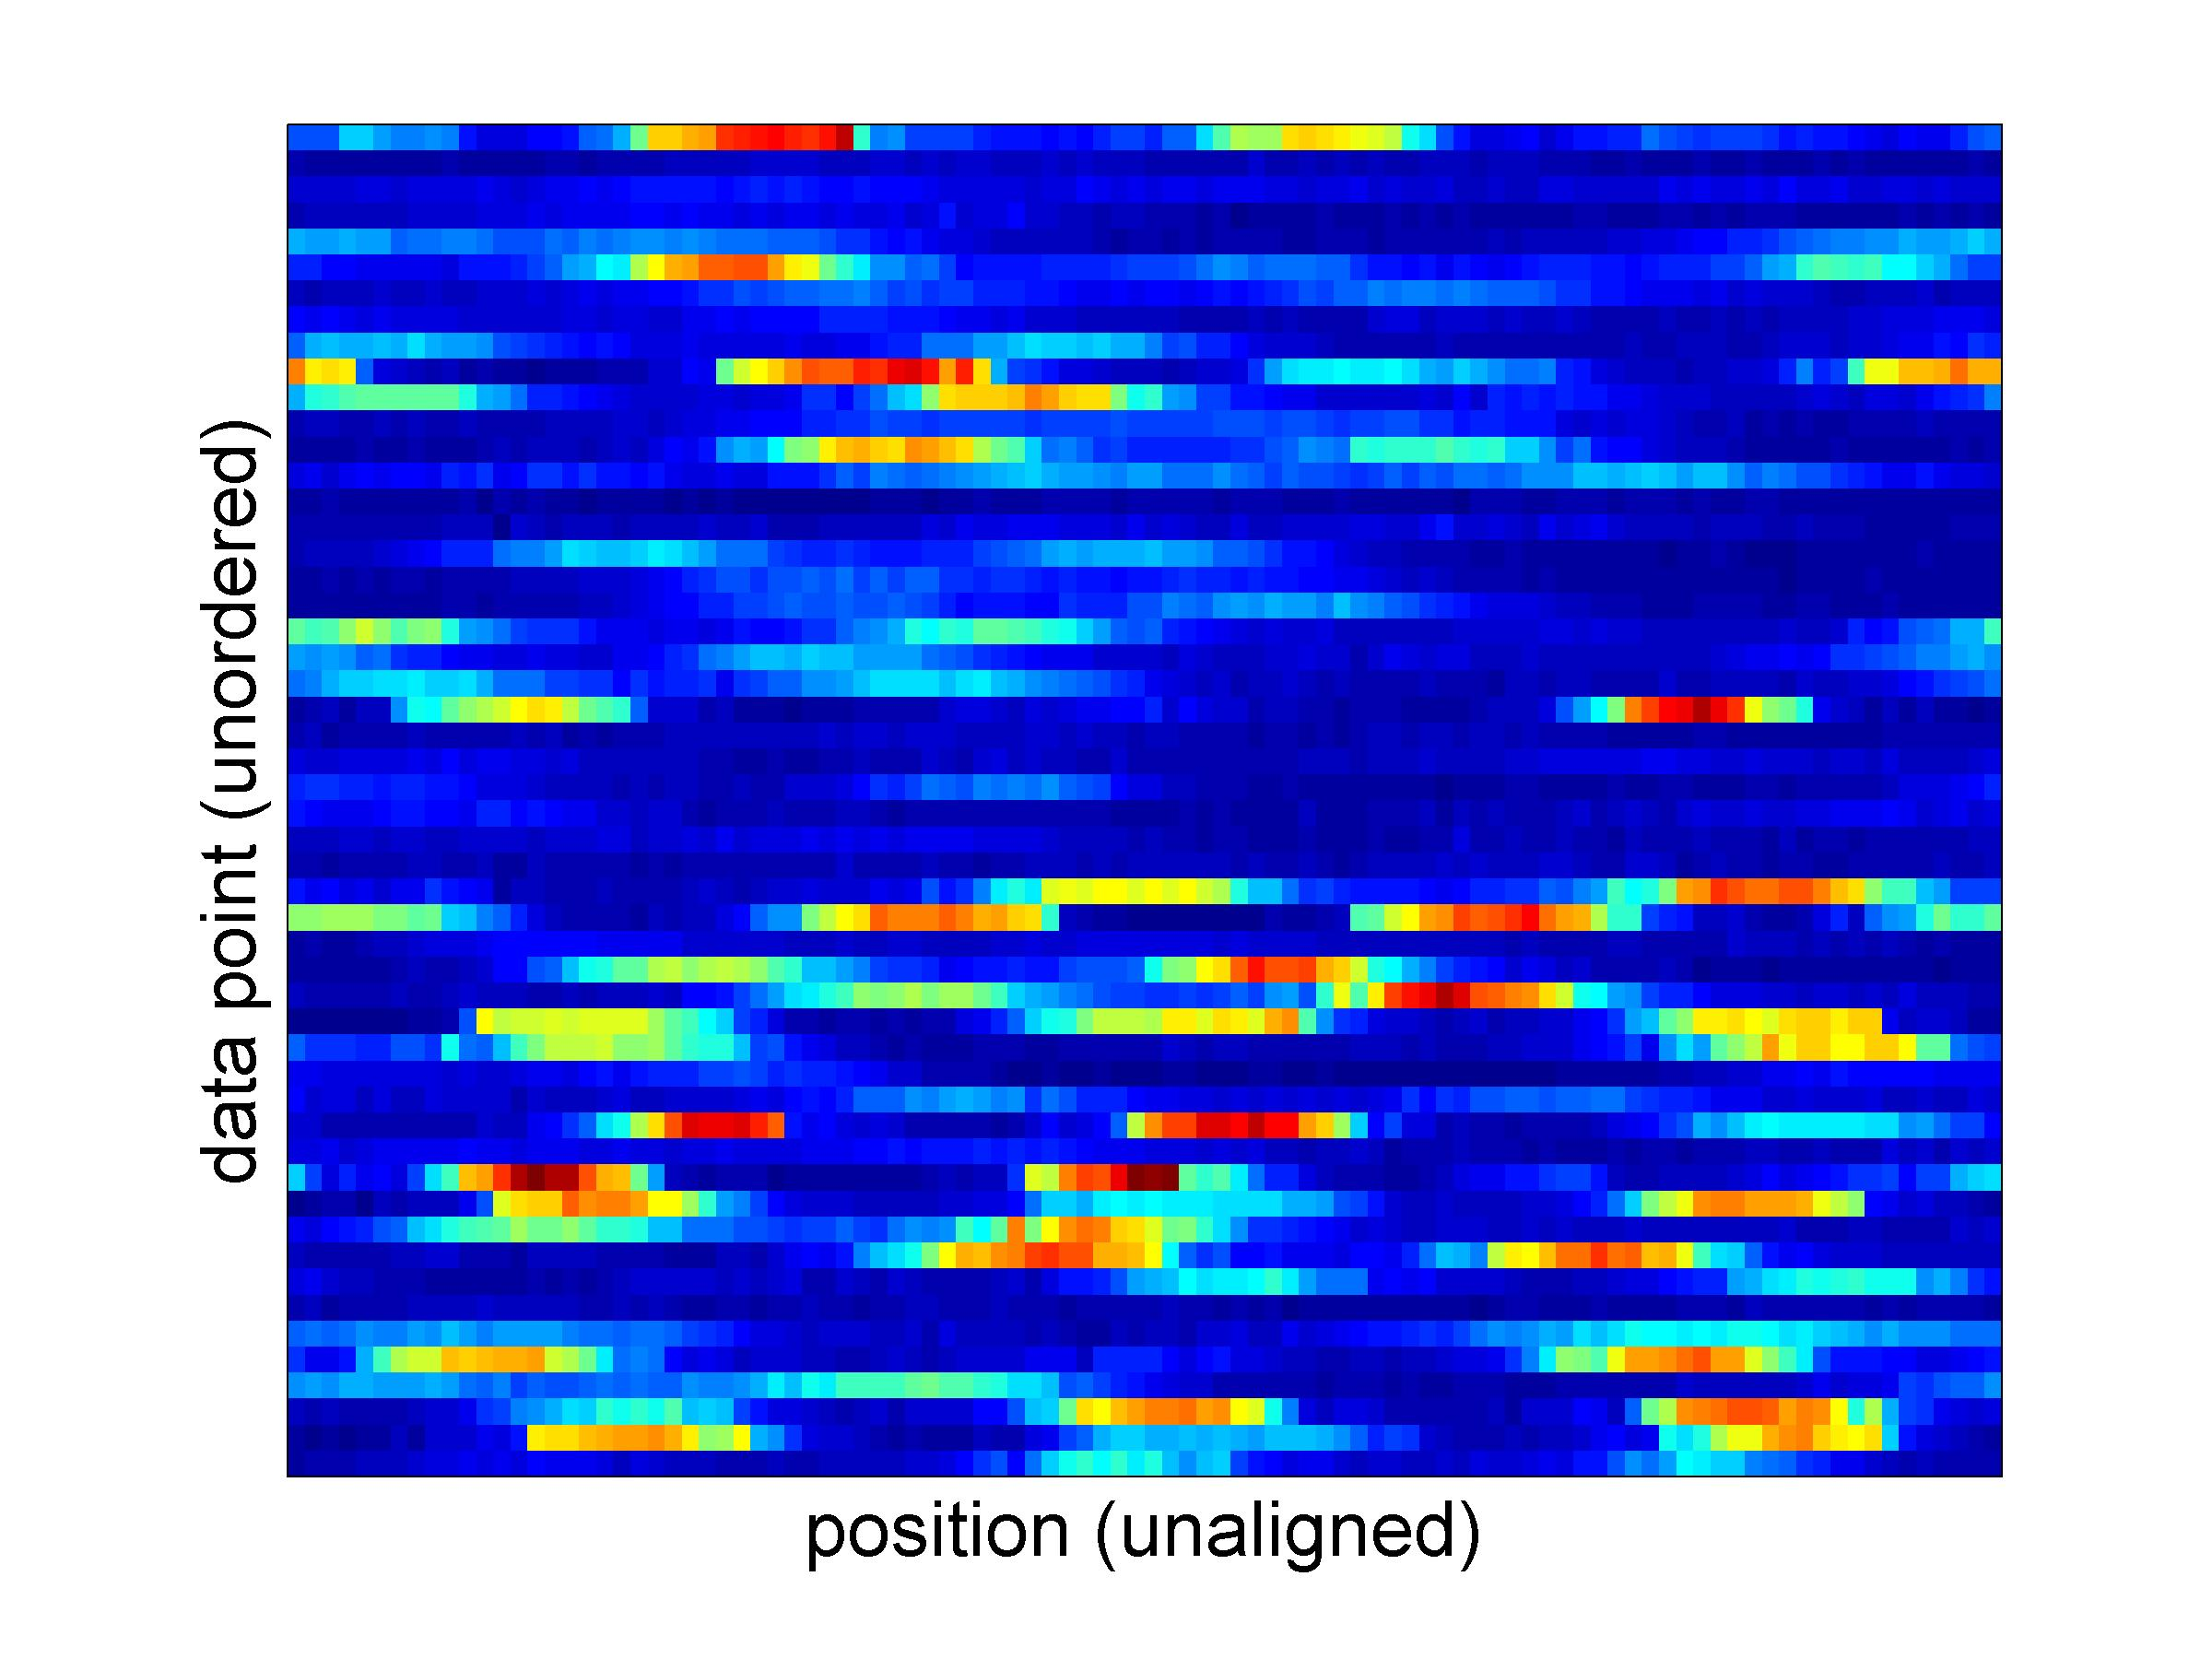
\includegraphics[width=\textwidth]{data_unaligned_unordered}
\caption{}
\end{subfigure}
\begin{subfigure}{0.3\textwidth}
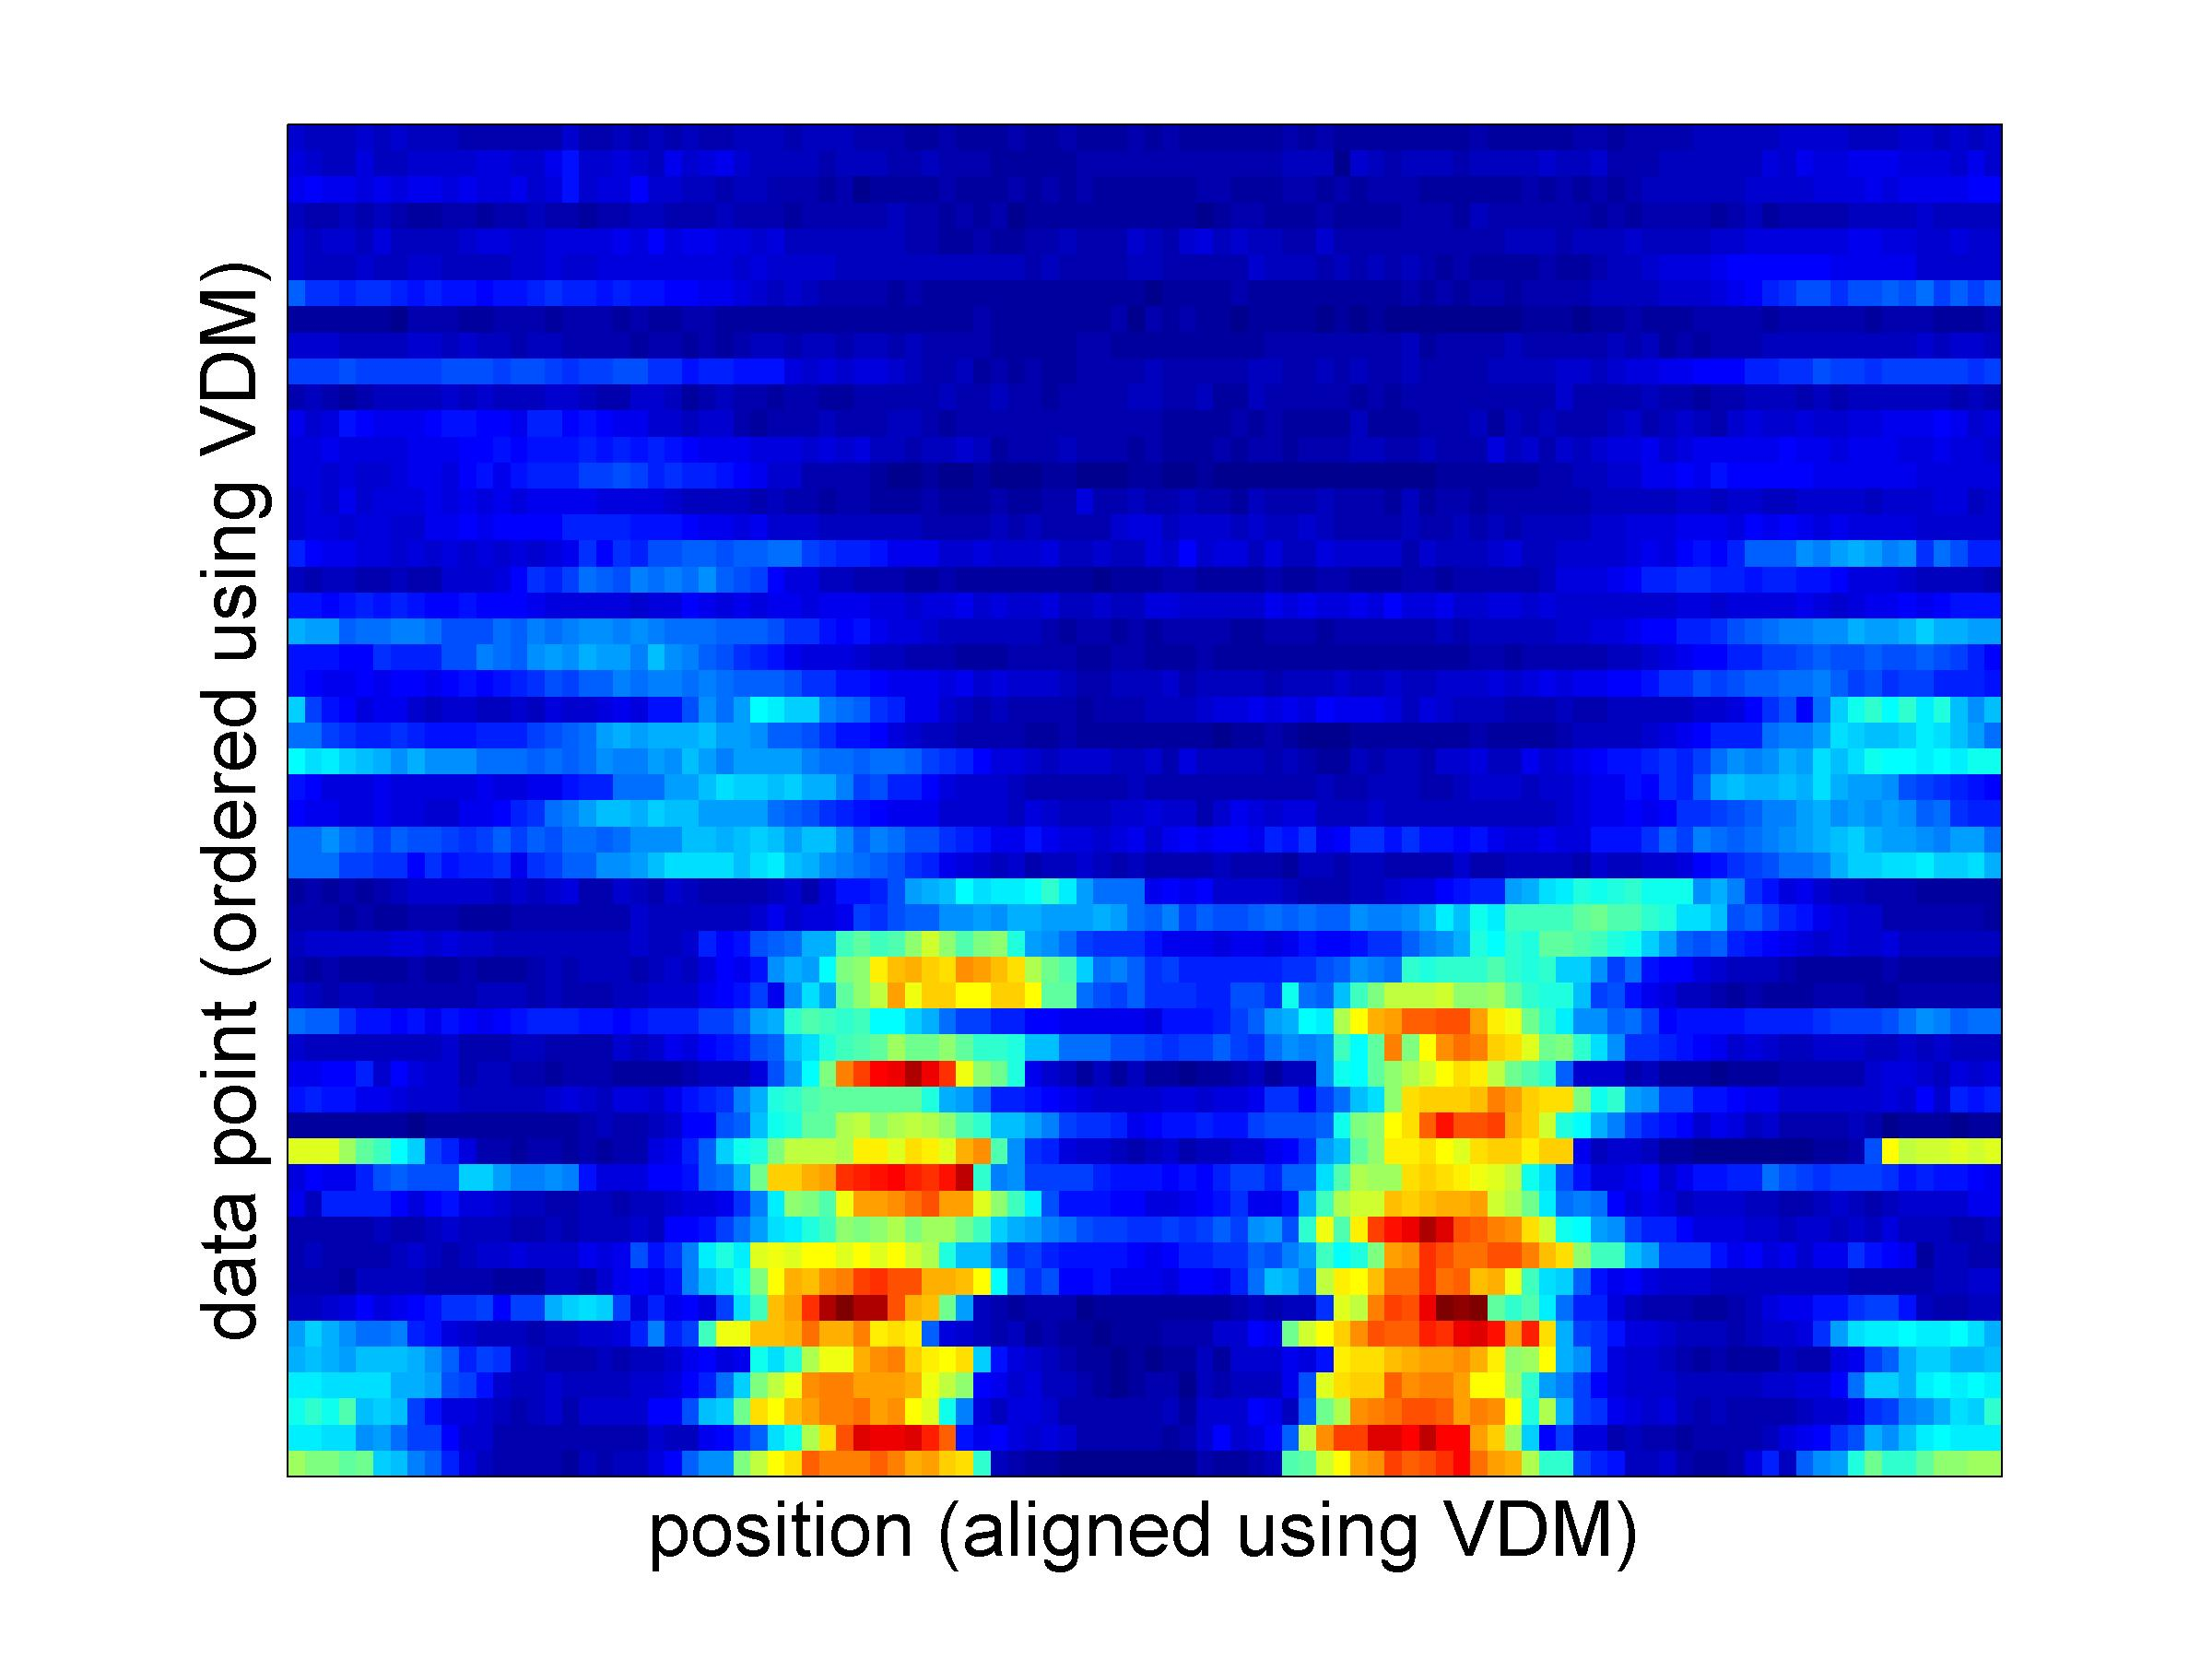
\includegraphics[width=\textwidth]{data_ordered_vdm}
\caption{}
\end{subfigure}
\begin{subfigure}{0.3\textwidth}
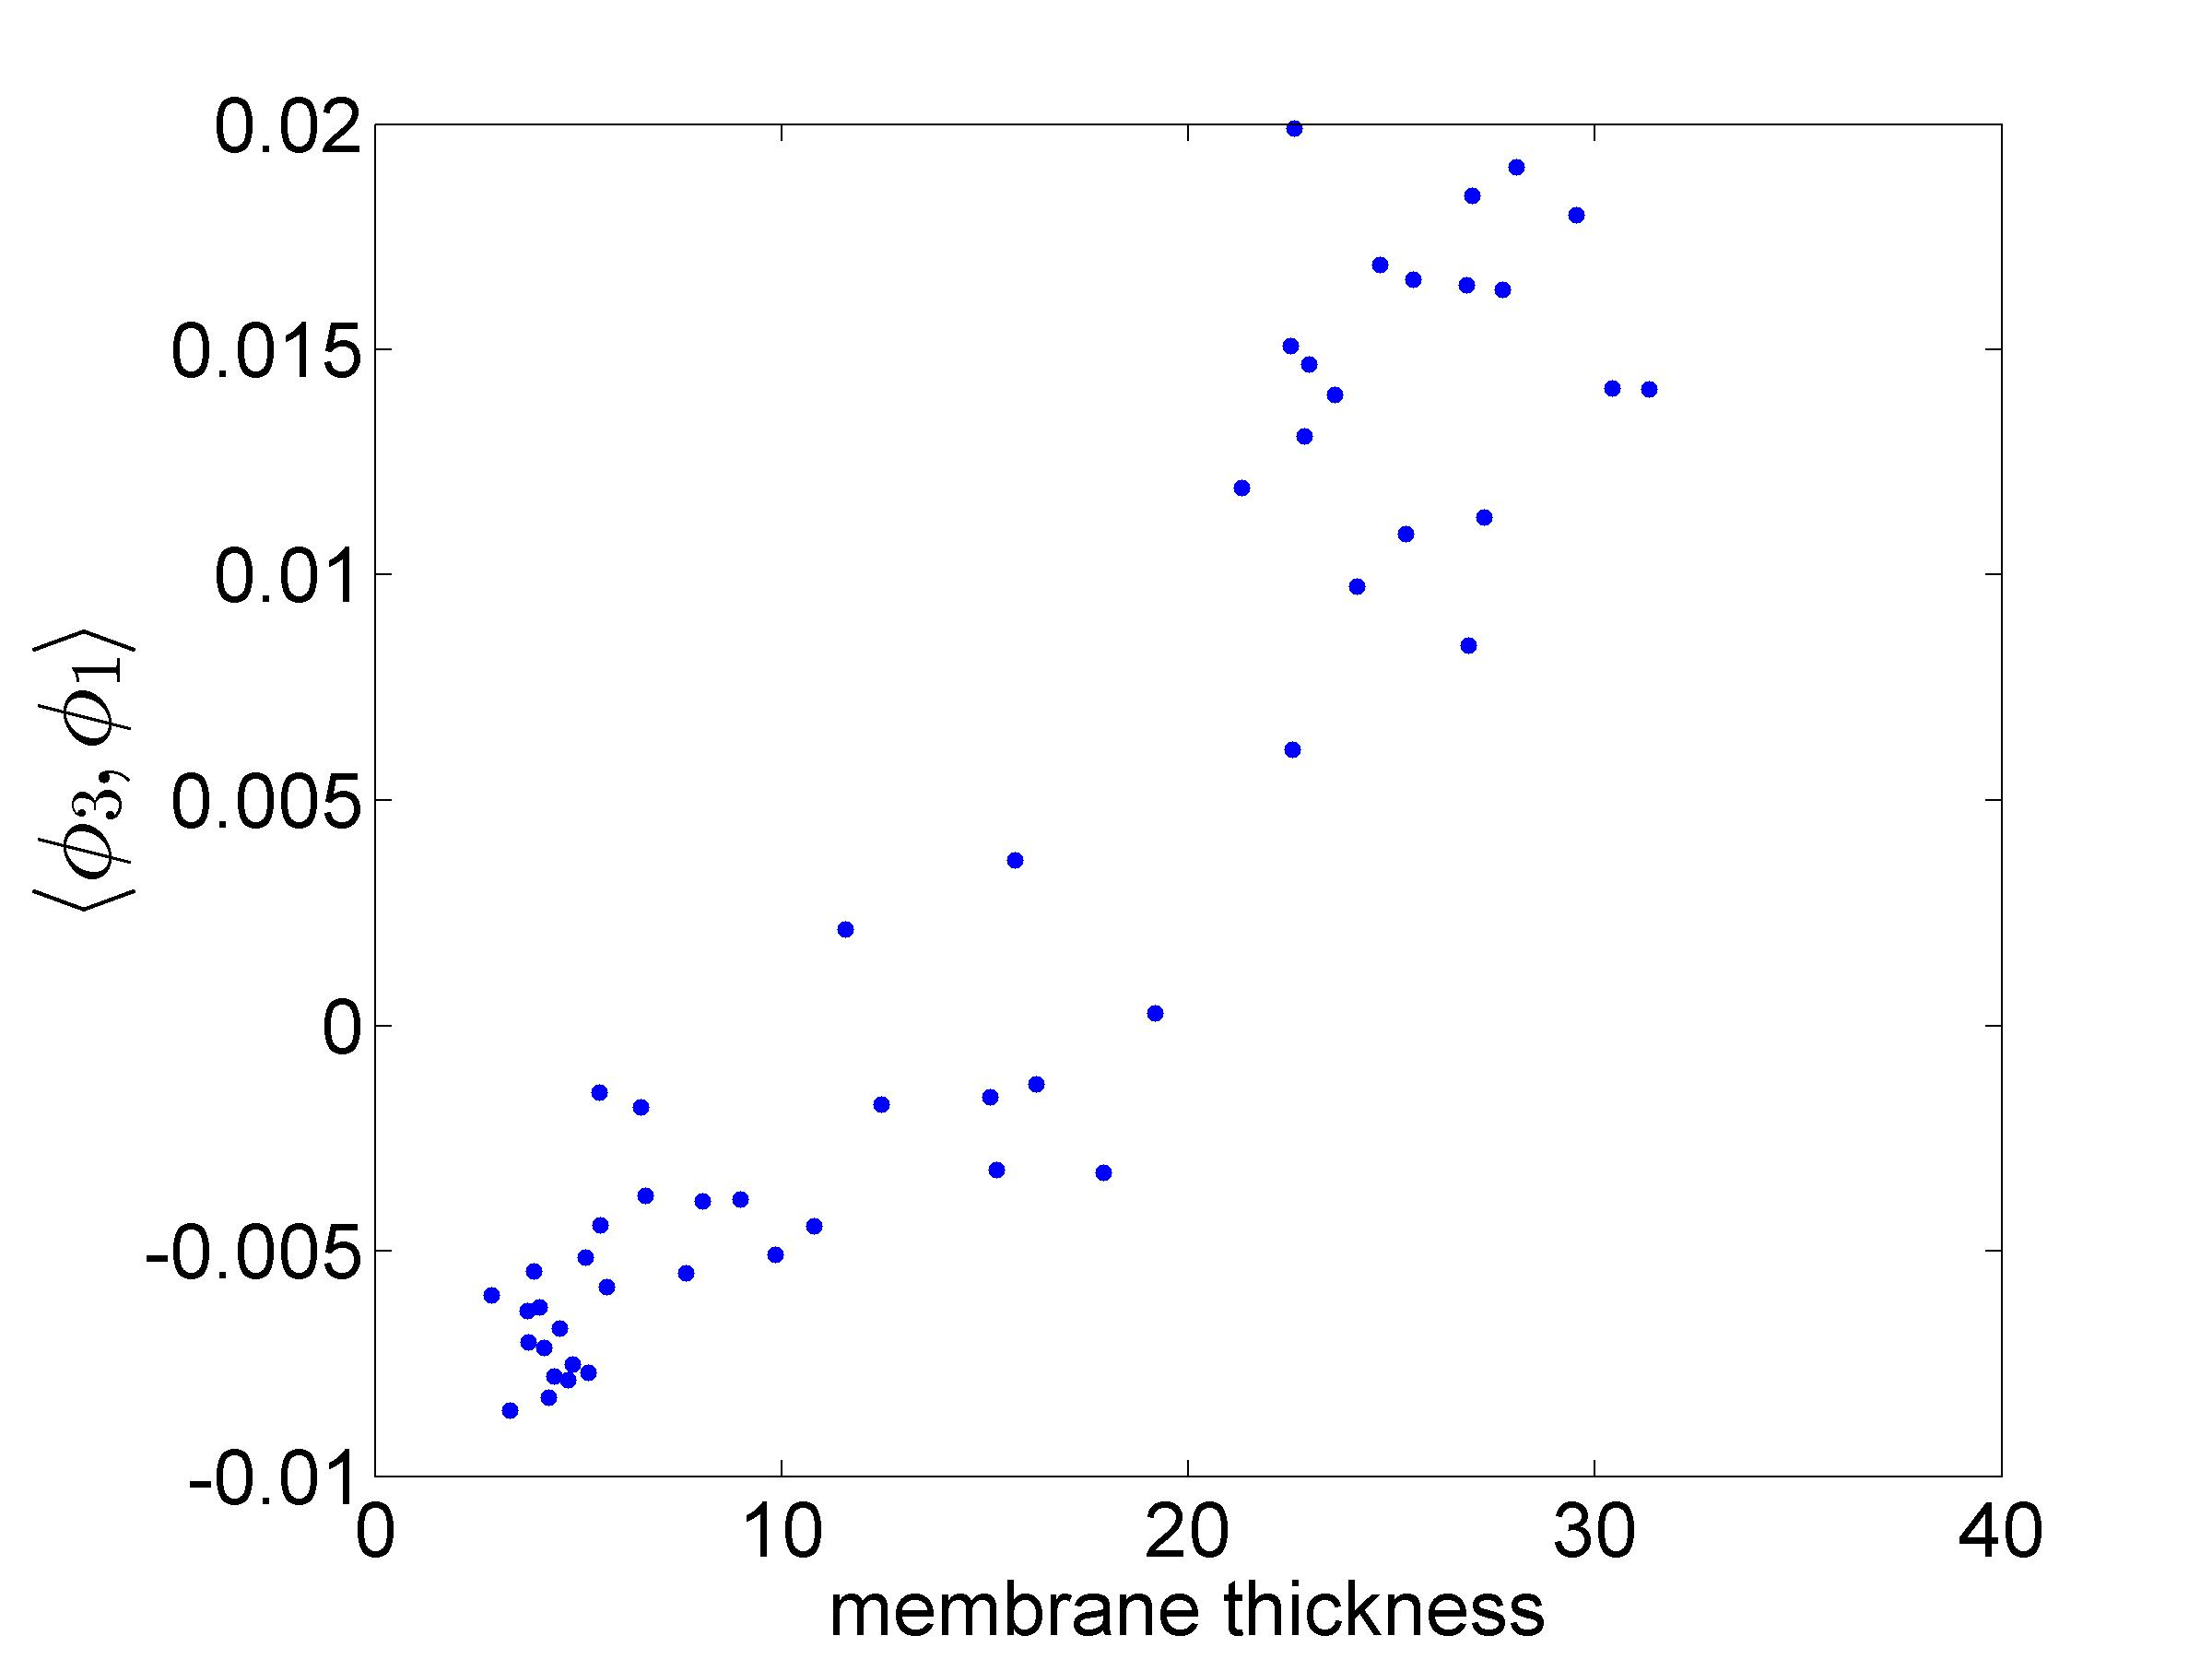
\includegraphics[width=\textwidth]{VDM_time_corr}
\caption{}
\end{subfigure}
\caption{{\bf Ordering spatially unaligned dpERK concentration profiles using vector diffusion maps.} (a) Concentration profiles of dpERK for many embryos. Each row represents a different embryo fixed at a slightly different developmental time. The circluar profiles have not been ``opened'' at the same point; rather, each profile was opened at a random point around the embryo. We are allowed to shift the (linear) profiles left and right.
(b) Concentration profiles of dpERK aligned and ordered using vector diffusion maps.
(c) Correlation between the VDM embedding coordinate and the membrane thickness.}
\label{fig:vdm_ordering}
\end{figure}

\subsection*{Two-dimensional dpERK images aligned and ordered using vector diffusion maps}

Thus far, we have focused on the one-dimensional linear concentration profiles that are extracted from the fluorescent images.
%
However, the techniques we have outlined can also be applied to the two-dimensional fluorescent images. 
%
We used VDM to align and order the dpERK fluorescent images. 
%
We now must factor out translations and rotations in the images. 
%
We first projected the images onto a sphere;
rotations and translations of a two-dimensional image then correspond to (three-dimensional) rotations of the sphere.
%
We used VDM to align and order the (projected) images, with the underlying symmetry group $SO(3)$. 
%
The results are shown in Figure \ref{fig:vdm_image_ordering};
the orderings are of comparable quality to those obtained with the one-dimensional profiles, and the dpERK peaks are nicely aligned.
%
The Spearman correlation between $\langle \phi_4, \phi_1 \rangle$ and the membrane length is 0.9051.

\def\imageindices{1,19,25,30,35,40,45,49}
%\def\imageindices{1,9,17,25,30,34,38,43,49}

\begin{figure}[!ht]
\centering
\begin{subfigure}{\textwidth}
\centering
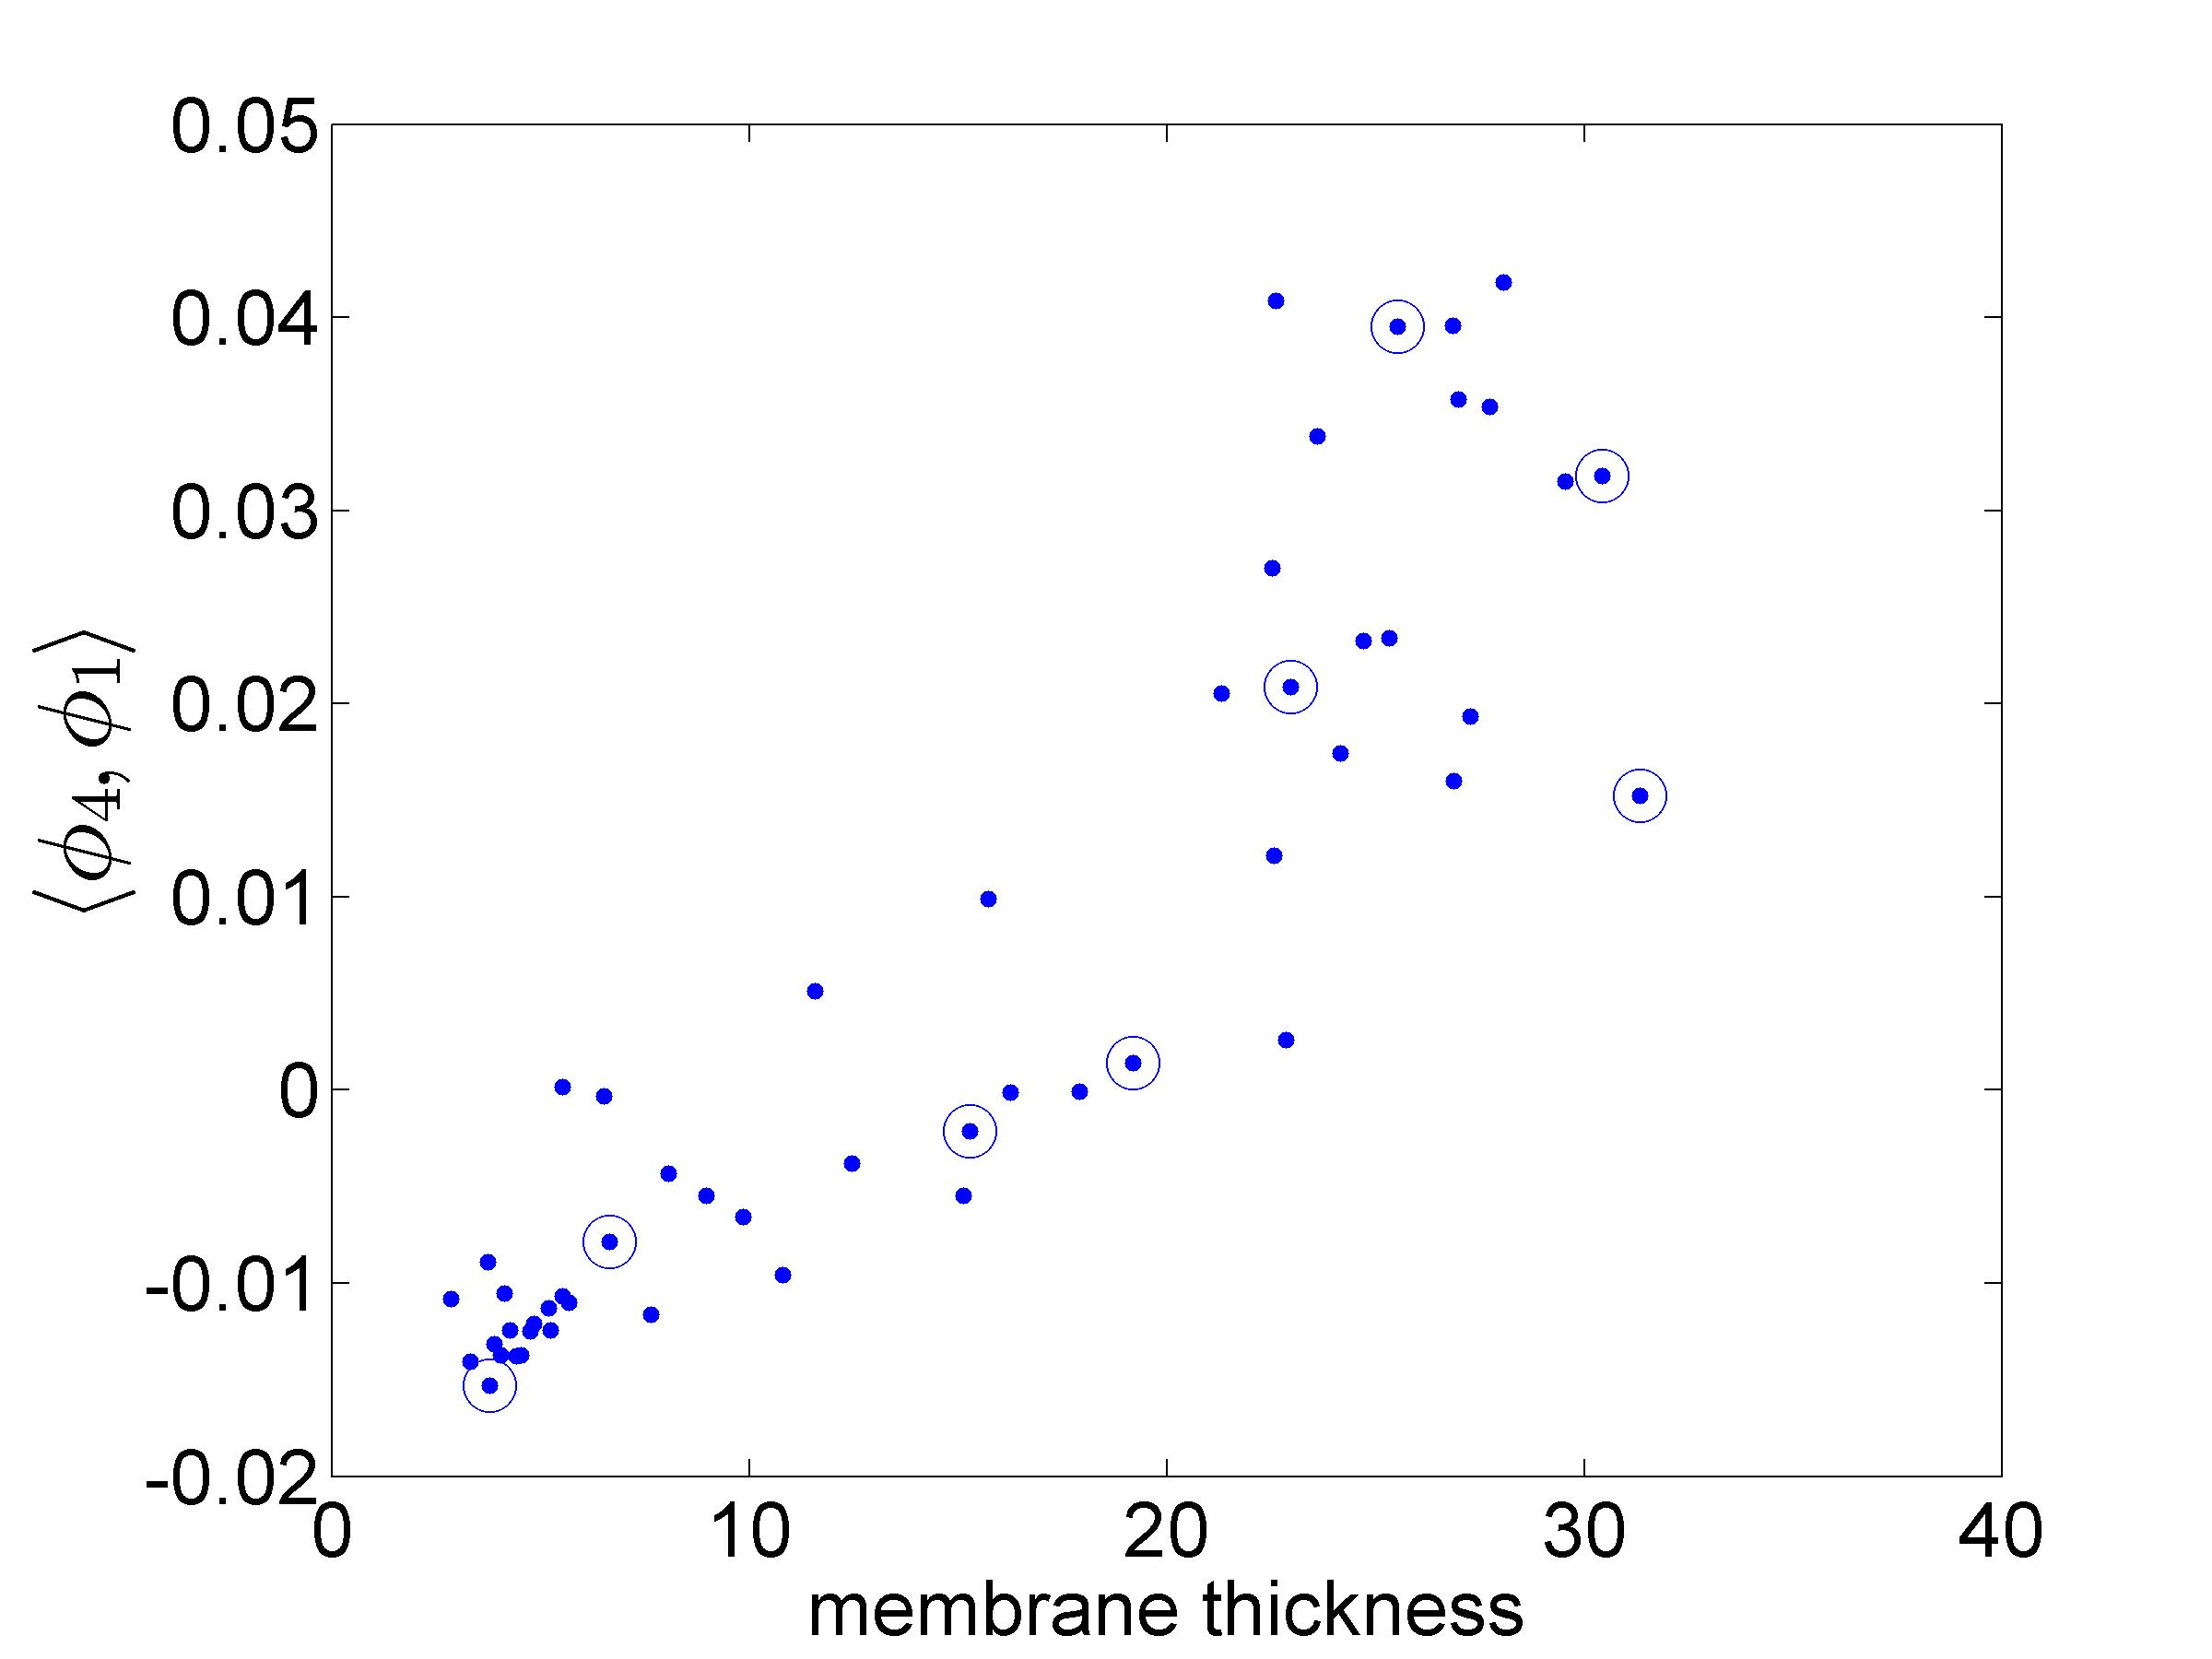
\includegraphics[width=0.7\textwidth]{vdm_2d_time_corr}
\caption{}
\end{subfigure}
\begin{subfigure}{\textwidth}
\foreach \n in \imageindices{
\includegraphics[width=0.1\textwidth]{dpERK_vdm_\n}
\hfill}
\caption{}
\end{subfigure}
\caption{{\bf Ordering two-dimensional fluorescent images of dpERK.}
(a) Correlation between the VDM embedding coordinate and the membrane thickness. 
(b) Some representative fluorescent images, aligned  and ordered using the VDM embedding coordinate. The corresponding data points are circled in (a). }
\label{fig:vdm_image_ordering}
\end{figure}

\subsection*{Two-dimensional dpERK images ordered using diffusion maps and the scattering transform}

An alternative to aligning the data (as in angular synchronization or VDM) is to construct {\em features} that are invariant to the underlying symmetry group, and then compute distances between features of the data for use in a DMAPS calculation.
%
In our setup, we require features of two-dimensional images that are invariant to translations and rotations of the images.
%
We chose to use the scattering transform \cite{mallat2012group} to construct our invariant features; the scattering transform utilizes a series of wavelet transforms, which are known to perform well for images \cite{akansu2010emerging}.
%
Not only is this transform invariant to translations and rotations, but is also a contractive operator \cite{bruna2011classification}, so that noise and small deformations are not amplified by the transform.

We compute the scattering transform coefficients for each image in our data set.
%
We then perform a DMAPS calculation, using the Euclidean distance between vectors of scattering transform coefficients as our distance metric.
%
The results are shown in Figure \ref{fig:scattrans_dpERK_ordering}.
%
The ordering is again good, with a Spearman correlation between $\phi_2$ and the membrane length of 0.9011.
%
However, we would like to note that using this method, we do not obtain optimal alignments for the images (we only obtain an ordering).

\begin{figure}[!ht]
\centering
\begin{subfigure}{\textwidth}
\centering
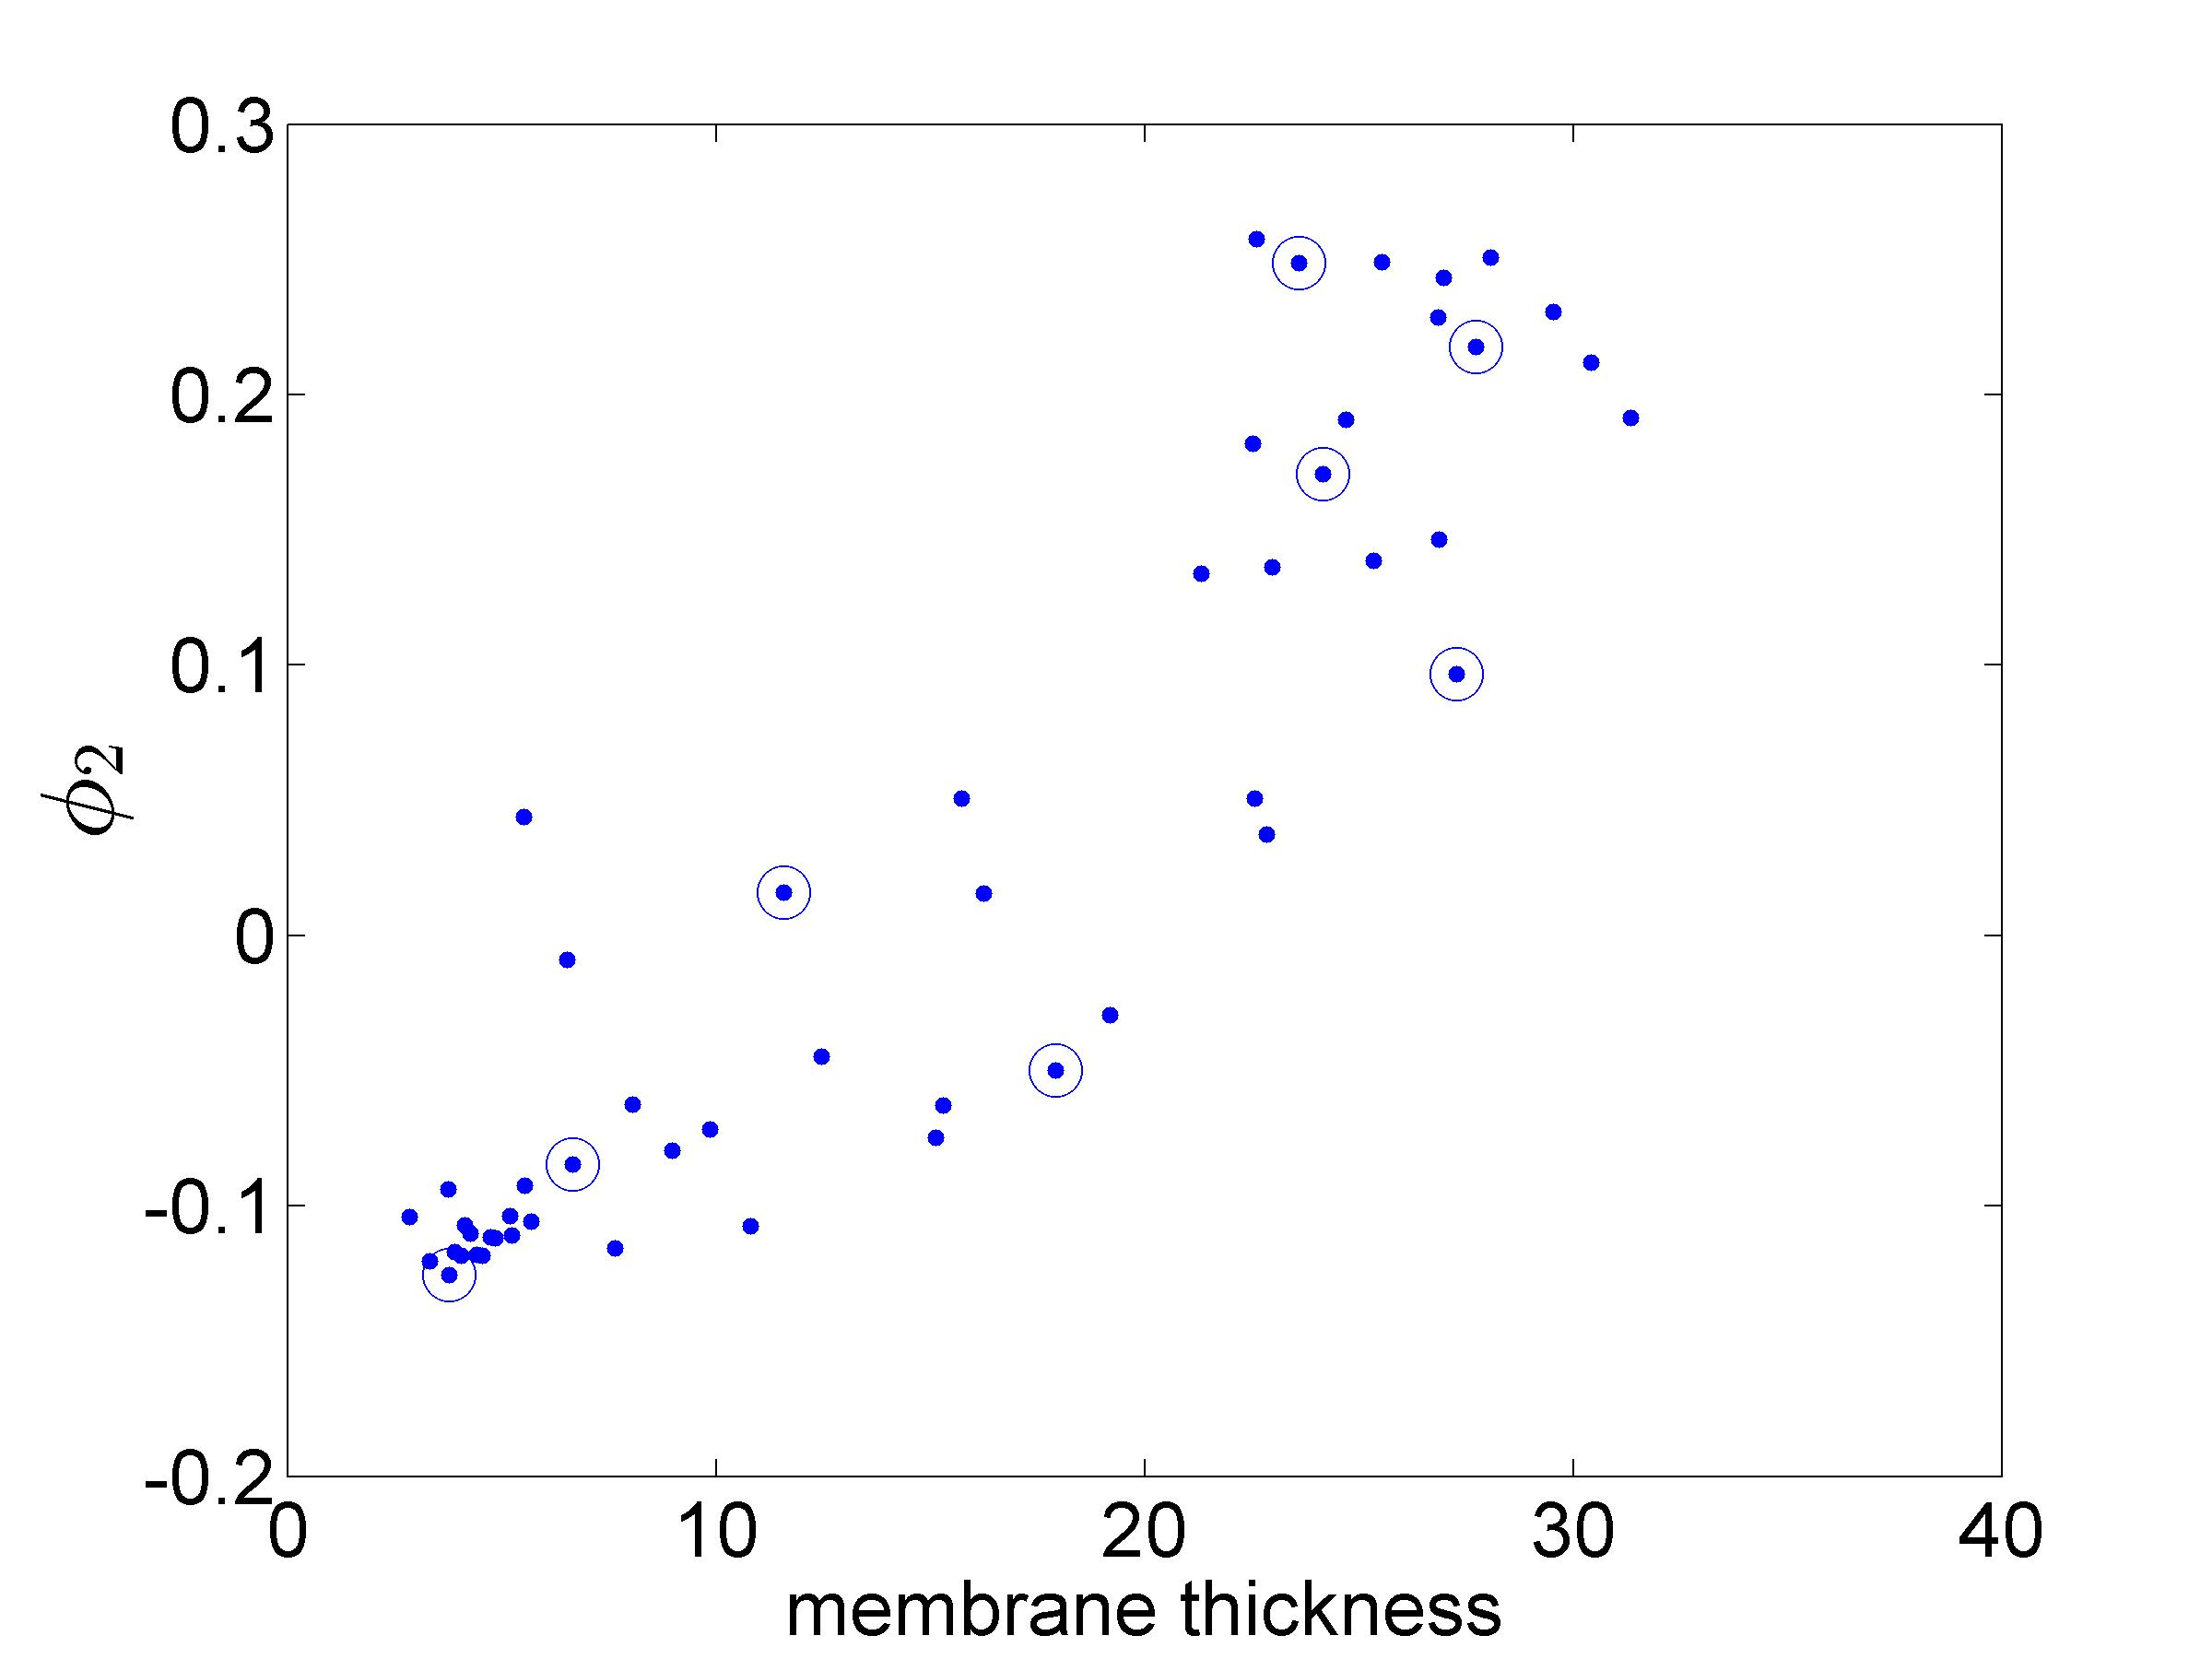
\includegraphics[width=0.7\textwidth]{DMAPS_scat_time_corr}
\caption{}
\end{subfigure}
\begin{subfigure}{\textwidth}
\foreach \n in \imageindices{
\includegraphics[width=0.1\textwidth]{dpERK_scat_\n}
\hfill}
\caption{}
\end{subfigure}
\caption{{\bf Ordering two-dimensional fluorescent images of dpERK.}
(a) Correlation between the first (non-trivial) DMAPS embedding coordinate and the membrane thickness. The DMAPS embedding was computed using the translation- and rotation-invariant scattering transform coefficients as ``features'' of the images.
(b) Some representative fluorescent images, ordered using the first (non-trivial) DMAPS embedding coordinate computed from the scattering transform coefficients. The corresponding data points are circled in (a).}
\label{fig:scattrans_dpERK_ordering}
\end{figure}

\subsection*{Two-dimensional membrane images ordered using diffusion maps and the scattering transform}

Thus far, we have focused on ordering the dpERK fluorescent images. 
%
However, we used the membrane thickness in Figure~\ref{fig:background} to order the dpERK concentration profiles. 
%
Therefore, we could also use the techniques discussed above to order the two-dimensional {\em membrane} images.
%
Because we are only interested in the membrane thickness, and not other features of the images (e.g. fluorescent intensity), we preprocess the images using an edge detection filter.
%
Some of these images are shown in Figure~\ref{fig:scattrans_membrane_ordering}; the green fluorescent images are those collected from the confocal microscope, and the grayscale images are the result of applying the edge-detection algorithm. 

Because these images are much more complex than the dpERK fluorescent images, we expect any alignment results to be poor.
%
Using VDM to align and order the images yielded a Spearman correlation coefficient of 0.3525.
%
However, the scattering transform is robust to small deformations, and so we expect using DMAPS with the scattering transform coefficients to give better results.
%
We computed the scattering transform coeffficients of the edge-detected images, and used DMAPS to order the images in time. 
%
The results are shown in Figure~\ref{fig:scattrans_membrane_ordering}.
%
The correlation between $\phi_2$ and the membrane thickness is not as strong as the correlations for the dpERK images; the Spearman correlation is 0.8403.
%
However, these results are still promising considering the relative simplicity of the methods. 
%
%$\rho = 0.8403$, 300 seconds for scat + DMAPS
%$\rho = 0.3525$ for VDM + membrane pics, 1100 seconds

\begin{figure}[!ht]
\centering
\begin{subfigure}{\textwidth}
\centering
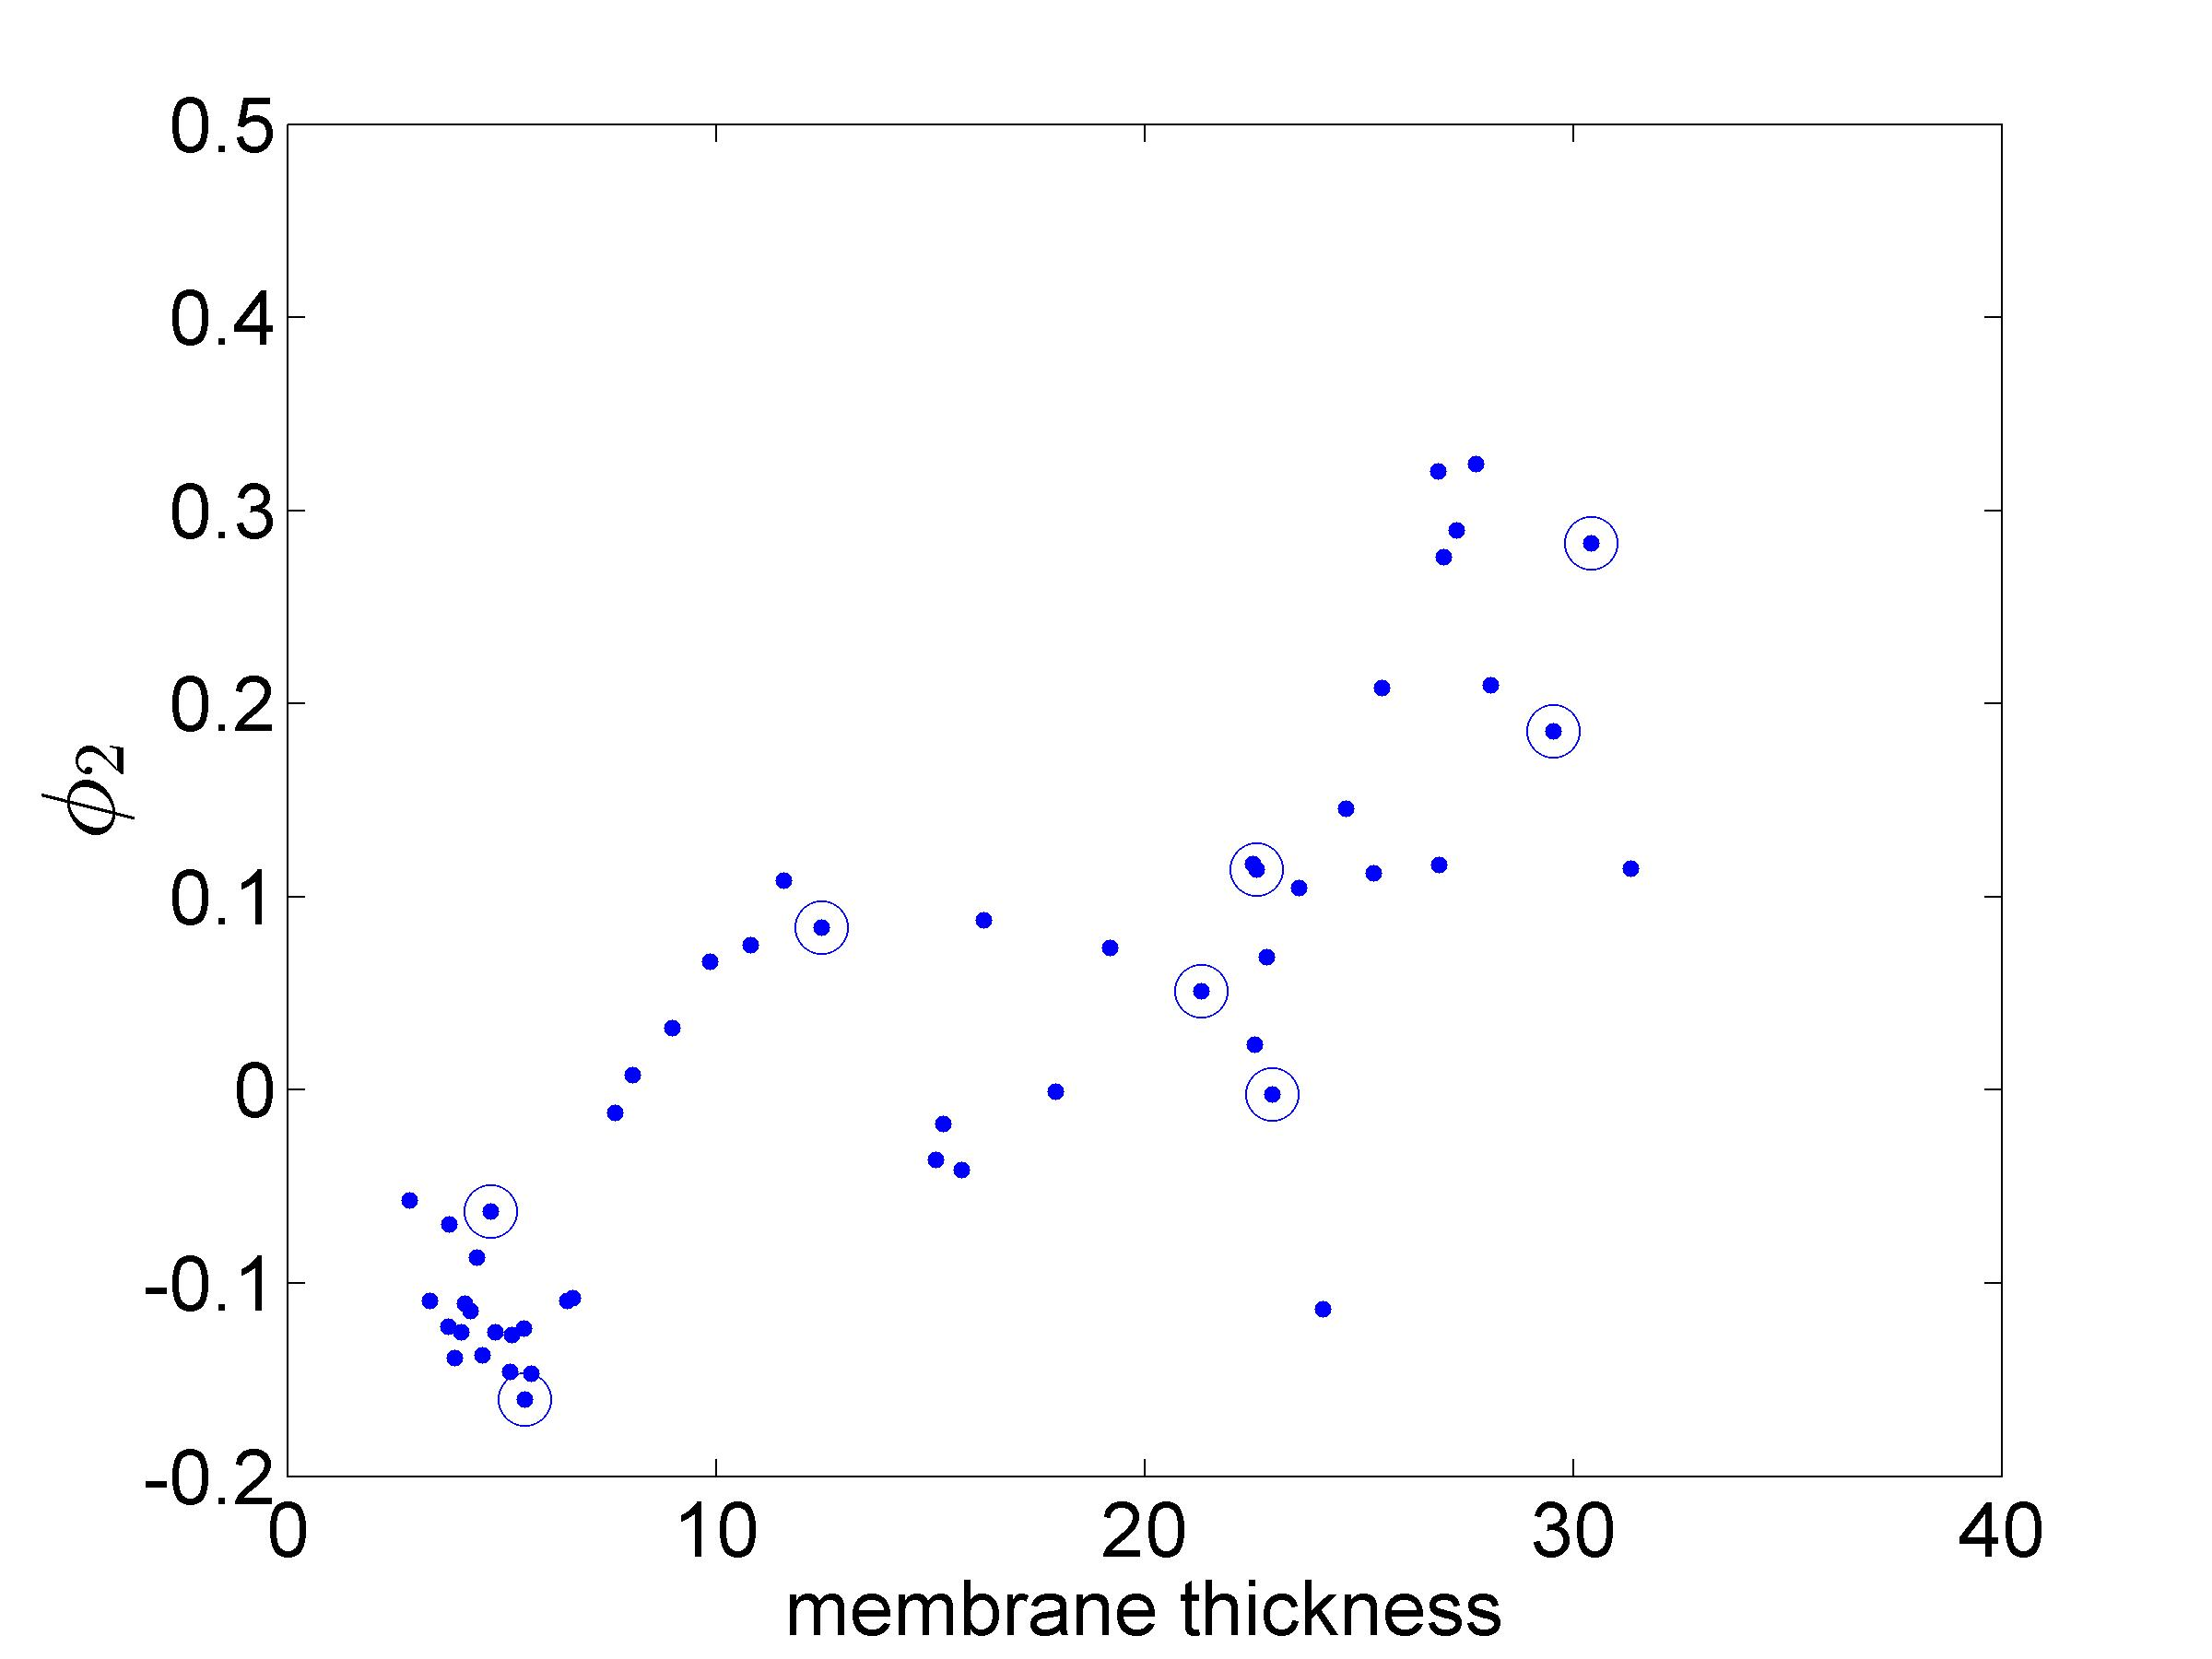
\includegraphics[width=0.7\textwidth]{DMAPS_membrane_scat_time_corr}
\caption{}
\end{subfigure}
\begin{subfigure}{\textwidth}
\foreach \n in \imageindices{
\includegraphics[width=0.1\textwidth]{membrane_scat_\n}
\hfill}
\newline
\foreach \n in \imageindices{
\includegraphics[width=0.1\textwidth]{membrane_scat_raw_\n}
\hfill}
\caption{}
\end{subfigure}
\caption{{\bf Ordering two-dimensional fluorescent images of membrane proteins.}
(a) Correlation between the seventh (non-trivial) DMAPS embedding coordinate and the membrane thickness. DMAPS was computed using the translation- and rotation-invariant scattering transform coefficients as ``features'' of the images. The first six non-trivial DMAPS coordinates were found to capture other features of the images, such as  differences in fluorescence intensity within the images.
(b) Some representative edge-detected images (top) and fluorescent images (bottom), ordered using the first (non-trivial) DMAPS embedding coordinate computed from the scattering transform coefficients. The corresponding data points are circled in (a).}
\label{fig:scattrans_membrane_ordering}
\end{figure}


\section*{Discussion}

We hope we have demonstrated the utility of dimensionality reduction techniques in systems with underlying symmetries and dynamics.
%
The work here is intended to provide an overview of the different techniques available, as well as the benefits and shortcomings of each method. 
%
The techniques were presented from least complex (PCA) to most complex (scattering transforms).
%
More complex techniques allowed us to deal with more complex data, and allowed us to circumvent much of the preprocessing described in Figure~\ref{fig:background}.

The more complex techniques that operate on two-dimensional images do come at a higher computational cost. 
%
The computational time for analyzing the one-dimensional profiles using any of the techniques described (PCA, DMAPS, angular synchronization, VDM) is less than one second. 
%
In contrast, the analysis of two-dimensional images using either VDM or the scattering transform with DMAPS is $\mathcal{O}(100)$ seconds.
%
The expensive portion of the VDM calculation is computing the pairwise alignments of the images, and the expensive portion of the scattering transform with DMAPS is computing the scattering transform coefficients.
%
However, computing the pairwise alignments is $\mathcal{O}(n^2)$, where $n$ is the number of data points, while computing the scattering transform coefficients is $\mathcal{O}(n)$.
%
We therefore expect for VDM to be computationally intractable for large data sets.
%
The added computational cost of VDM is not without benefits; VDM produces optimal alignments for each image (in addition to an ordering), while the scattering transform gives us no alignments.

We would like to note that our system was such that the data was inherently one-dimensional, and that this one dimension was monotonic in time.
%
However, this monotonicity was a special feature of our system and is not guaranteed in general.
%TODO: add more conclusions


%\begin{table}
%	\begin{tabular}{| p{0.3\textwidth} | c | c | p{0.3\textwidth} |}
%		\hline 
%		Method & Spearman's $\rho$ & Execution Time & Notes About Method \\ 
%		\hline 
%		PCA on one-dimensional profiles & 0.9244 & $< 1$ second & \\
%		\hline 
%		DMAPS on one-dimensional profiles & 0.9209 & $< 1$ second & \\
%		\hline 
%		Angular synchronization + DMAPS on one-dimensional profiles & 0.9164 & $< 1$ second & \\
%		\hline 
%		VDM on one-dimensional profiles & 0.9232 & $< 1$ second & \\	
%		\hline 
%		VDM on two-dimensional images & 0.9051  & $325$ seconds & $\mathcal{O}(n^2)$ to compute the pairwise alignments\\
%		\hline 	
%		Scattering transform + DMAPS on two-dimensional profiles & 0.9011  & $86$ seconds &  $\mathcal{O}(n)$ to compute the scattering transform for each data point \\
%		\hline
%		Scattering transform + DMAPS on two-dimensional membrane images & 0.8403  & $300$ seconds &  $\mathcal{O}(n)$ to compute the scattering transform for each data point \\
%		\hline
%	\end{tabular}
%\end{table}
% You may title this section "Methods" or "Models".
% "Models" is not a valid title for PLoS ONE authors. However, PLoS ONE
% authors may use "Analysis"
\section*{Materials and Methods}

\subsection*{Experimental setup}

\subsection*{Image preprocessing}
The dpERK images we collected from the confocal microscope were subsampled to $100 \times 100$ pixels; 
the membrane images were subsampled to $200 \times 200$ pixels (due to the finer structure in the membrane pictures). 
%
Because we were only interested in the membrane thickness, we ran a simple edge detection algorithm on the membrane images.
%
We used a Laplacian of Gaussians filter \cite{canny1986computational}, as implemented in the Matlab Image processing toolbox via the \texttt{edge} function (\url{http://www.mathworks.com/help/images/ref/edge.html}).
%
To compute the pairwise alignments between images for use in angular synchronization and VDM, we searched over 20 rotations (evenly spaced from $0$ to $2 \pi$) and 10 translations spanning $\pm 10 \%$ of the image pixels.
%
We used the Euclidean distance between images to measure the quality of the alignment.
%
These translations and rotations were then converted to three-dimensional rotations on the sphere, with the image spanning a $\pi/4 \times \pi/4$ portion of the sphere.%, so that the angle of rotation of the image corresponded to the Euler angle $\alpha$, $pixels_x/pixels_{max} * \pi/4$ corresponded to the Euler angle $\beta$, and  $pixels_y/pixels_{max} * \pi/4$ corresponded to the Euler angle $\gamma$.

\subsection*{Spearman's rank correlation coefficient}

Spearman's rank correlation coefficient, or Spearman's $\rho$, measures the monotonicity of a function \cite{myers2010research}. 
%
It therefore serves as an appropriate metric for the quality of our orderings.
%
Given two data sets $X$ and $Y$, with data points $X_i$ and $Y_i$, we compute the ranks of each data point within the data set, denoted $x_i$ and $y_i$.
%
Spearman's rank correlation between $X$ and $Y$ is then defined as the correlation between the ranks
\begin{equation}
\rho = \frac{\sum_i (x_i - \overline{x})(y_i - \overline{y})}{\sqrt{\sum_i (x_i - \overline{x})^2 \sum_i (y_i - \overline{y})^2}}
\end{equation}
where $\overline{x}$ and $\overline{y}$ are the averages of $x_i$ and $y_i$, respectively. 

\subsection*{Principal component analysis}
Principal component analysis (PCA) has been the workhorse dimensionality reduction technique for the past century.
%
PCA finds the optimal planes or hyperplanes on which to project the data in order to maximize the variance of the projected data \cite{shlens2005tutorial}.

Let $X \in \mathbb{R}^{n \times d}$ denote our data set, consisting of $n$ points in $d$ dimensions, where $X_{ij}$ denotes the $j^{th}$ dimension of the $i^{th}$ observation. 
%
We first mean-center the data set to produce the matrix $\hat{X}$, where
\begin{equation}
\hat{X}_{ij} = X_{ij} - \frac{1}{n} \sum_{k=1}^n X_{kj}.
\end{equation}
%
The empirical covariance of the data set, $C \in \mathbb{R}^{d \times d}$ is then given by
\begin{equation}
C = X^T X.
\end{equation}
%
We compute the eigenvectors $\psi_1, \dots, \psi_d$ and eigenvalues $\lambda_1, \lambda_2, \dots, \lambda_d$ of $C$, and order them such that $\lambda_1 \ge \lambda_2 \ge \dots \ge \lambda_d$.
%
The principal components of the data set $X$ are given by $\psi_1, \dots, \psi_d$, and the eigenvalues $\lambda_1, \lambda_2, \dots, \lambda_d$ measure the variability captured by the corresponding eigenvector. 
%
If there is a {\em spectral gap} such that the first few eigenvectors capture a significant portion of the variance in our data set, projection onto these first few principal components will retain most features of the data set while reducing the dimensionality.
%
In our setup, we assume that the data is inherently one-dimensional, and that projection onto $\psi_1$ will uncover the correct time ordering of the data.

\subsection*{Diffusion maps}
Unlike PCA, diffusion maps (DMAPS) is a nonlinear dimensionality reduction technique. 
%
DMAPS aims to uncover a parameterization of high-dimensional data sampled from a low-dimensional nonlinear manifold \cite{coifman2005geometric}.
%
The {\em essential} requirement for DMAPS is an appropriate distance metric $d(x_i, x_j)$ for comparing data points. 
%
This can as simple as the standard Euclidean distance, or a more complex metric (such as a distance between features of the data points) for other data sets.

Given data points $x_1, \dots, x_n \in \mathbb{R}^d$, we fist calculate the matrix $W \in \mathbb{R}^{n \times n}$, where 
\begin{equation}
W_{ij} = \exp \left( -\frac{d^2(x_i, x)j)}{\epsilon} \right)
\end{equation}
and $\epsilon$ is a characteristic distance between data points.
%
$\epsilon$ can be chosen using several techniques (see, for example \cite{coifman2008graph}); in practice, we choose $\epsilon$ to be the median of the pairwise distances between data points.
%
We then compute the diagonal matrix $D$, where $D_{ii} = \sum_{j=1}^{n} W_{ij}$, and the matrix $A = D^{-1} W$. 
%
We calculate the eigenvectors $\phi_1, \phi_2, \dots, \phi_n$ and eigenvalues $\lambda_1, \lambda_2, \dots, \lambda_n$ and order them such that $|\lambda_1| \ge |\lambda_2| \ge \dots \ge |\lambda_n|$. 
%
Because the matrix $A$ is similar to the symmetric matrix $D^{-1/2} W D^{-1/2}$, $A$ is guaranteed to have real eigenvalues and real, orthogonal eigenvectors. 
%
The eigenvectors $\phi_1, \phi_2, \dots, \phi_n$ give the embedding coordinates, such that $\phi_j(i)$ gives the $j^{th}$ embedding coordinate of the $i^{th}$ data point. 
%
Because the matrix $A$ is row-stochastic, $\lambda_1=1$ and $\phi_1$ is a constant vector; the next few eigenvectors give the ``meaningful'' embedding coordinates for the data. 

\subsection*{Angular synchronization}

When the data set is invariant under an underlying symmetry group (such as rotations), we must first factor out the underlying symmetries before doing further analysis.
%
Angular synchronization calculates the optimal alignments for a data set, assuming we have estimates of the optimal alignments between pairs of data points \cite{singer2011angular}. 

Let $x_1, \dots, x_n$ denote the data points that we wish to align under some symmetry group.
%
We will consider the case where the symmetry group is the group of $d$-dimensional rotations, $SO(d)$. 
%
Let $R_{ij} \in SO(d)$ denote the rotation that aligns $x_j$ to $x_i$, so that
\begin{equation}
R_{ij} = \argmin_{R \in SO(d)} \|Rx_j - x_i \|^2.
\end{equation}
%
We seek to find the rotations $R_1, R_2, \dots, R_n \in SO(d)$ such that $R_i R_j^T \approx R_{ij}$, for every pair $i, j$. 
%TODO: Check that this order is correct
%
We would also like to exploit {\em higher-order} consistency relations;
for example, the relationship $R_{ij} R_{jk} R_{ki} = I$, where $I$ is the identity matrix, should hold.
%
Therefore, we consider measurements which (almost) satisfy such conditions ``good'' measurements, and those measurements which do not satisfy such conditions as most likely inaccurate.

We define the objective function 
\begin{equation} \label{eqn:angsynch_obj}
\max_{R_1, \dots, R_n \in SO(d)} \sum_{i=1}^{n} \sum_{j=1}^{n} R_i^T R_{ij} R_j.
\end{equation}
%
%TODO: check if a norm is needed
This objective function is large if $R_i$ adn $R_j$ are consistent with $R_{ij}$, and will be random with mean 0 if $R_i$ and $R_j$ are inconsistent with $R_{ij}$.
%
Therefore, we are seeking the most consistent set of global alignments, given the computed pairwise alignments.

In general, the solution to \eqref{eqn:angsynch_obj} is not easily computed.
%
Instead, we relax the problem and allow $R_1, \dots, R_n \in \mathbb{R}^{d \times d}$.
%
We then define the matrix $H$, which is an $n \times n$ block matrix with $d \times d$ blocks (so $H \in \mathbb{R}^{nd \times nd}$).
%
We then compute the top ``block'' eigenvector of $H$, which we denote $\hat{R} \in \mathbb{R}^{nd \times d}$. 
%
The solution to the relaxed problem is given by $\hat{R}$, so that the $i^{th}$ rotation is (approximately) $\hat{R}(i) \in \mathbb{R}^{d \times d}$.
%
This formulation also accounts for higher-order relations.
%
For example, if we want to optimize over all pairs of pairwise rotations, we would solve $\max_{R_1, \dots, R_n \in SO(d)} \sum_{i=1}^{n} \sum_{j=1}^{n} R_i^T \left( \sum_k R_{ik} R_{kj} \right) R_j$. 
%
However, the solution to this problem is also given by the top eigenvector of $H$. 

Because we relaxed the problem to allow our solutions to lie in $\mathbb{R}^{d \times d}$, we must project our approximate solution back to $SO(d)$.
%
The optimal rotation is therefore given by $R_i = U_i V_i^T$, where $U_i$ and $V_i$ are the left and right singular vectors of $\hat{R}_i$, respectively. 

\subsection*{Vector diffusion maps} 

Angular synchronization assumes that each data point is a replicate measurements of the same underlying configuration, simply corrupted with rotations and some noise.
%
However, in system with an underlying symmetry group {\em as well as} a dynamical process, the data points are not identical modulo symmetries and noise, and we would like to place more emphasis on aligning data points which are dynamically close.

Vector diffusion maps (VDM) couples the symmetry-factoring of angular synchronization with the uncovering of dynamics of diffusion maps \cite{singer2012vector}. 
%
We construct the matrix $A$ as in diffusion maps, and the matrix $H$ as in angular synchronization.
%
We then construct the block matrix $S$, where the blocks of $S$ are defined by
\begin{equation}
S_{ij} = \left\{ \begin{array}{l l} 
A_{ij} H_{ij} & i \ne j \\
0_{d \times d} & i = j
\end{array}
\right.
\end{equation}
%
where $A_{ij}$ is the $(i,j)$ entry of $A$, and $H_{ij}$ is the $(i,j)$ block of $H$. 

We then compute the eigenvectors $\phi_1, \dots, \phi_{nd}$ and eigenvalues $\lambda_1, \dots, \lambda_{nd}$ of $S$, and order them such that $|\lambda_1| \ge |\lambda_2| \ge \dots \ge |\lambda_{nd}|$.
%
As in angular synchronization, the first ``block'' eigenvector, i.e. the first two eigenvectors concatenated into a $nd \times d$ matrix, gives the optimal rotations. 
%
However, the eigenvectors now also give us embedding coordinates.
%
Let $\phi_j(i)$ denote the $i^{th}$ block of $\phi_j$. 
%
The embedding coordinates are then given by $\langle \phi_j(i), \phi_k(i) \rangle$, where $1 \le j, k, \le nd$. 

\subsection*{Scattering transform}

The scattering transform consists of a wavelet transform of the signal, followed by  the appropriate averaging operator.
%
This transform is applied to the signal itself, as well as to the residual, in order to preserve as much information about the signal itself, while still keeping the transform coefficients translation- and rotation-invariant. 
% 
Furthermore, the scattering transform can be shown to be a contractive operator; therefore, noise and small deformations in the signal are not amplified in the transformation.
%
We utilized the freely available ScatNet software (\url{http://www.di.ens.fr/data/software/scatnet/}) to compute the rotation-invariant scattering coefficients. 

% Do NOT remove this, even if you are not including acknowledgments
\section*{Acknowledgments}


%\section*{References}
% The bibtex filename
\bibliography{../../references/references}

%\section*{Figure Legends}
%\begin{figure}[!ht]
%\begin{center}
%%\includegraphics[width=4in]{figure_name.2.eps}
%\end{center}
%\caption{
%{\bf Bold the first sentence.}  Rest of figure 2  caption.  Caption
%should be left justified, as specified by the options to the caption
%package.
%}
%\label{Figure_label}
%\end{figure}


%\section*{Tables}
%\begin{table}[!ht]
%\caption{
%\bf{Table title}}
%\begin{tabular}{|c|c|c|}
%table information
%\end{tabular}
%\begin{flushleft}Table caption
%\end{flushleft}
%\label{tab:label}
% \end{table}

\end{document}
